\documentclass[acmlarge]{acmart}

\usepackage{booktabs} % For formal tables
\usepackage[ruled]{algorithm2e} % For algorithms
\usepackage{colortbl}
\usepackage{subfigure}
\usepackage{multirow}
\usepackage{enumitem}
\usepackage{rotating}
%\usepackage{times}  %time new roman type
\usepackage{url}
\usepackage{subfigure}
\usepackage{multirow}
\usepackage{tabularx}
\usepackage{diagbox}
\usepackage{color}

\newcommand{\systemname}{SleepGuard}
\definecolor{Gray}{gray}{0.9}
\newcommand{\etal}{\emph{et al.}}

\SetAlFnt{\small}
\SetAlCapFnt{\small}
\SetAlCapNameFnt{\small}
\SetAlCapHSkip{0pt}
\IncMargin{-\parindent}

% Metadata Information
%%% Revise this part at the final submission
\acmJournal{IMWUT}
\acmVolume{2}
\acmNumber{3}
\acmArticle{39}
\acmYear{2018}
\acmMonth{9}
\acmArticleSeq{11}
% Copyright
\setcopyright{acmcopyright}
%\setcopyright{acmlicensed}
%\setcopyright{rightsretained}
%\setcopyright{usgov}
\setcopyright{usgovmixed}
%\setcopyright{cagov}
%\setcopyright{cagovmixed}
\acmPrice{15.00}

%%% Revise this part at the final submission
\acmDOI{0000001.0000001}

% Paper history
%% Uncomment and revise this part at the final submission
\received{February 2018}
\received{May 2018}
\received[accepted]{August 2018}



\begin{document}

\title{\systemname: Capturing Rich Sleep Information using Smartwatch Sensing Data}
%\titlenote{We can add a note to the title}

%%% Uncomment  this part at the final submission
%\author{Liqiong Chang, Jiaqi Lu, Ju Wang, Xiaojiang Chen, Dingyi Fang, Zhanyong Tang}
%%\authornote{This is the corresponding author}
%\orcid{1234-5678-9012-3456}
%\affiliation{
%	\institution{Northwest University}
%	\country{China}} \email{{clq, jqlu, wangju, xjchen, dyf, zytang}@nwu.edu.cn}
%
%\author{Petteri Nurmi, Zheng Wang}
%\affiliation{
%	\institution{Lancaster University}
%	\country{United Kingdom}} \email{{p.nurmi, z.wang}@lancaster.ac.uk}

%NOTE: This is supposed to be anonymous review.

\begin{abstract}
Sleep is an important part of our daily routine -- we spend about one-third of our time doing it. By tracking sleep-related events and
activities, sleep monitoring provides decision support to help us understand sleep quality and  causes of poor sleep. Wearable devices
provide a new way for sleep monitoring, allowing us to monitor sleep from the comfort of our own home. However, existing  solutions do
not take full advantage of the rich sensor data provided by these devices. In this paper, we present the design and development of
{\systemname}, a novel approach to track a wide range of sleep-related events using smartwatches. We show that using merely a single
smartwatch, it is possible to capture rich amount of information about sleep events and sleeping context, including body posture and
movements, acoustic events, and illumination conditions. We demonstrate that through these events it is possible to estimate sleep
quality and identify factors affecting it most. We evaluate our approach by conducting extensive experiments involved fifteen users
across a 2-week period. Our experimental results show that our approach can track a richer set of sleep events, provide better decision
support for evaluating sleep quality, and help to identify causes for sleep problems compared to prior work. %We also show that
%{\systemname} can help users to improve their sleep quality by having a better understanding of the root causes of sleep problems.
\end{abstract}


\begin{CCSXML}
	<ccs2012>
	<concept>
	<concept_id>10003120.10003138</concept_id>
	<concept_desc>Human-centered computing~Ubiquitous and mobile computing</concept_desc>
	<concept_significance>500</concept_significance>
	</concept>
	</ccs2012>
\end{CCSXML}

\ccsdesc[500]{Human-centered computing~Ubiquitous and mobile computing} \keywords{Smartwatch sensing; mobile sensing; sleep events; sleep
monitoring}


\begin{CCSXML}
	<ccs2012>
	<concept>
	<concept_id>10003120.10003138</concept_id>
	<concept_desc>Human-centered computing~Ubiquitous and mobile computing</concept_desc>
	<concept_significance>500</concept_significance>
	</concept>
	</ccs2012>
\end{CCSXML}

\ccsdesc[500]{Human-centered computing~Ubiquitous and mobile computing}

\keywords{Smartwatch, Sleep Events, Sensing}

%\thanks{This work is partially supported by the xxx.}

\maketitle

%\renewcommand{\shortauthors}{L. Chang et al. }


\section{INTRODUCTION}\label{sec:1introduction}

Sleep plays a vital role in good health and personal well-being throughout one's life. Lack of sleep or poor quality of sleep can lead to serious, sometimes life-threatening, health problems~\cite{altena2008sleep,chandola2010effect,lallukka2016contribution}, decrease level of
cognitive performance~\cite{alhola07sleep,akerstedt07altered}, and affect mood and feelings of personal
well-being~\cite{paunio09longitudinal,pilcher97sleep}. Besides having an adverse effect on individuals, insufficient or poor quality sleep has a significant economic burden, among others, through decreased productivity, and medical and social costs associated with treatment of sleep disorders~\cite{hafner17why}. Indeed, to highlight the significance of sleep quality, the Centre for Disease Prevention (CDC) has declared insufficient sleep as a public health problem in the US~\cite{sleepreport}, and the concern is widely shared amongst other industrialized countries.


Traditionally, sleep monitoring is performed in a clinical environment using Polysomnography (PSG). In PSG, medical
sensors attached to human body are used to monitor events and information such as respiration, electroencephalogram (EEG), electrocardiogram (ECG), electro-oculogram and oxygen saturation~\cite{ebrahimi2008automatic,saper2005hypothalamic,oropesa1999sleep,langkvist2012sleep}. These information sources can then be used to determine sleep stages, sleep efficiency, abnormal breathing, and overall sleep quality. PSG is widely considered as the gold standard for sleep monitoring, and while it is extensively used to support clinical treatments of sleep disorders, it has some disadvantages that make it unsuitable for longitudinal and large-scale sleep monitoring. Firstly, {attaching and outfitting} the sensing instruments is time-consuming and laborious, and they are prone to disrupting sleeping routines. Secondly, PSG is rather expensive to use and requires a clinical environment and highly trained medical professionals to operate. Due to these disadvantages, PSG is only suitable as a way to support severe disorders {where} clinical care is required.

Recently, sleep monitoring based on off-the-shelf mobile and wearable devices has emerged as an alternative way to obtain information about one's sleeping patterns~\cite{ko15consumer,shelgikar2016sleep}. By taking advantage of diverse sensors, behaviors and routines associated with sleeping can be captured and modelled. This in turn can help users understand their sleep behavior and provide feedback on how to improve sleep, for example, by changing routines surrounding sleep activity or improving the sleeping environment. What makes self monitoring particularly attractive is the non-invasive nature of the sensing compared to PSG. Examples of consumer-grade sleep monitors range from apps running on smartphones or tablets to smartwatches and specialized wearable devices~\cite{zeo,Jawbone,SleepAndroid,fitbit,gu2016sleep,sleepmonitor}.

Despite the popularity of consumer-grade sleep monitors, currently the full potential of these devices is not being realized. Indeed, while current consumer-grade sleep monitors can capture and model a wide range of sleep related information, such as estimating overall sleep quality, capturing different stages of sleep, and identifying specific events occurring during
sleep~\cite{kay2012lullaby,zhang2013real,sleepmonitor}, they offer little help in understanding the characteristics that surround poor sleep. Thus, these solutions are unable to capture the root cause behind poor sleep or to provide {actionable} recommendations on how to improve sleep quality. This is because current solutions focus on monitoring characteristics of the sleep itself, without considering behaviors occurring during sleep and the environmental context affecting sleep, e.g., ambient light-level and noise. Indeed, sleep quality has been shown to depend on a wide range of factors. For example, intensity of ambient light~\cite{hood04determinants} and noisiness~\cite{muzet2007environmental} of the environment can significantly affect sleep quality. Similarly, the user's breathing patterns, postures during sleep, and routines surrounding the bedtime also have a significant impact on sleep quality. Without details of the environment and activities across sleep stages, the root cause of poor sleep cannot be captured and the user informed of how to improve their sleep quality. To unlock the full potential of consumer-grade sleep monitoring, innovative ways to take advantage of the rich sensor data accessible through these devices are required.

The present paper contributes by presenting the design and development of {\systemname}, a \emph{holistic sleep monitoring solution} that captures rich information about sleep events, the sleep environment, and the overall quality of sleep. {\systemname} is the first to solely rely on sensor information available on off-the-shelf smartwatches for capturing a wide range of sleep-related activities (see Table~\ref{tab:test}). The key insight in {\systemname} is that sleep quality is strongly correlated with characteristics of body movements, health related factors that can be identified from audio information, and characteristics of the sleep environment~\cite{shelgikar2016sleep}. By using a smartwatch, the sensors are close to the user during all stages of the night, enabling detailed capture of not only sleep cycles, but body movements and environmental changes taking place during the sleep period. Capturing these sleeping events from sensor data, however, is non-trivial due to changes in sensor measurements caused by hand motions during sleep. To overcome this challenge, changes in sensor orientation relative to the user's body need to be tracked and opportune moments where to capture sensor data need to be detected.  {\systemname} addresses these issues by integrating a set of new methods for analyzing and capturing sleep-related information from sensor measurements available on a smartwatch. {\systemname} also incorporates a model that uses the detected events to infer the user's sleep stages and sleep quality. While some prior research has examined the use of smartwatches for sleep monitoring~\cite{pombo2016ubisleep,shelgikar2016sleep,haescher2015anomaly,borazio2012combining}, these approaches have only been able to gather coarse-grained information about sleep and often required additional highly-specialized devices, such as pressure mattresses or image acquisition equipment to supplement the measurements available from the smartwatch. In this paper, we demonstrate that, for the first time, using {\em only a smartwatch}, it is possible to capture an extensive set of sleep-related information -- many of which are not presented in prior work. Having a more comprehensive set of sleep-related events and activities available enables users to gain a deeper understanding of their sleep patterns and the causes of poor sleep, and to make recommendations on how to improve one's sleep quality.

We evaluate {\systemname} through rigorous and extensive benchmark experiments conducted on data collected from fifteen participants during a two week monitoring period. The results of our experiments demonstrate that {\systemname} can accurately characterize body motions and movements during sleep, as well as capture different acoustic events. Specifically, the lowest accuracy for {\systemname} in our experiments is 87\%, with the best event detection accuracy reaching up to 98\%. We also demonstrate that {\systemname} can accurately detect various sleep stages and help users to better understand their sleep quality. During our experiments, $6$ of the $15$ participants suffered from some sleep problems ($4$ with bad and $2$ with general sleep quality), all of whom were correctly identified by {\systemname}. Moreover, we also demonstrate that {\systemname} is able to correctly identify the root causes of sleep problems for the $4$ participants with bad sleep quality, whether it is due to suboptimal hand position, body posture or sleeping environment. Compared to state-of-the-art sleep monitoring systems, such as Fitbit and Sleep Hunter, the main advantage of {\systemname} is that can report a wider range of sleep events and provide a better understanding for the causes of sleep problems.

\begin{table}[!t]
 \caption{\label{tab:test}Sleep events targeted in this work}
 \centering
 \begin{tabular}{ll}
  %\toprule
  \toprule
  \textbf{Event}& \textbf{Type} \\
  \midrule
\rowcolor{Gray}  Sleep postures & Supine, Left lateral, Right lateral, Prone\\
 Hand positions & Head, Chest, Abdomen\\
\rowcolor{Gray} Body rollover & Count\\
 Micro body movements& Hand moving, Arm raising, Body trembling \\
\rowcolor{Gray} Acoustic events & Snore, Cough, Somniloquy  \\
 Illumination condition & Strong, Weak  \\
  \bottomrule
 %\hline
 \end{tabular}
\end{table}


%\subsection*{Contributions}
This paper makes the following contributions:

\begin{itemize}
	\item We present the design and development of {\systemname} (Sec. ~\ref{Sec:3design}), the first holistic sleep monitoring system to rely solely on sensors available in an off-the-shelf smartwatch to capture a wide range of sleep information that characterizes overall sleep quality, user behaviors during sleep, and the sleep environment.
	
\item We develop novel and lightweight algorithms for capturing sleep-related information on smartwatches taking into consideration changes in orientation and location of the device during different parts of the night. We show how to overcome specific challenges to effectively track events like sleep postures (Sec.~\ref{sec:sleeppdet}), hand positions (Sec.~\ref{sec:handpr}), body rollovers (Sec.~\ref{sec:bodyrollover}), micro body movements (Sec.~\ref{sec:microbo}), and acoustic events (Sec.~\ref{sec:acoustic}) and illumination conditions (Sec.~\ref{sec:illumination}).
	

    \item We extensively evaluate the performance of {\systemname} using measurements collected from two-week monitoring of $15$ participants (Sec.~\ref{sec:expsetup}). Our results demonstrate that {\systemname} can accurately capture a wide range of sleep events, estimate different sleep stages, and produce meaningful information about overall sleep quality (Sec.~\ref{sec:4experiment}).  We show that {\systemname} successfully reveals the causes of poor sleeps for some of our testing users and subsequently helps them improve their sleep by changing their sleep behaviors and sleeping environment  (Sec.~\ref{sec:user_survey}).
\end{itemize}

%ZW: I have commented out the motivation section as it reads like related work.
%\input{motivation.tex}
%%\subsection{Overview of \systemname}

%\begin{figure}
%  \centering
  % Requires \usepackage{graphicx}
 % 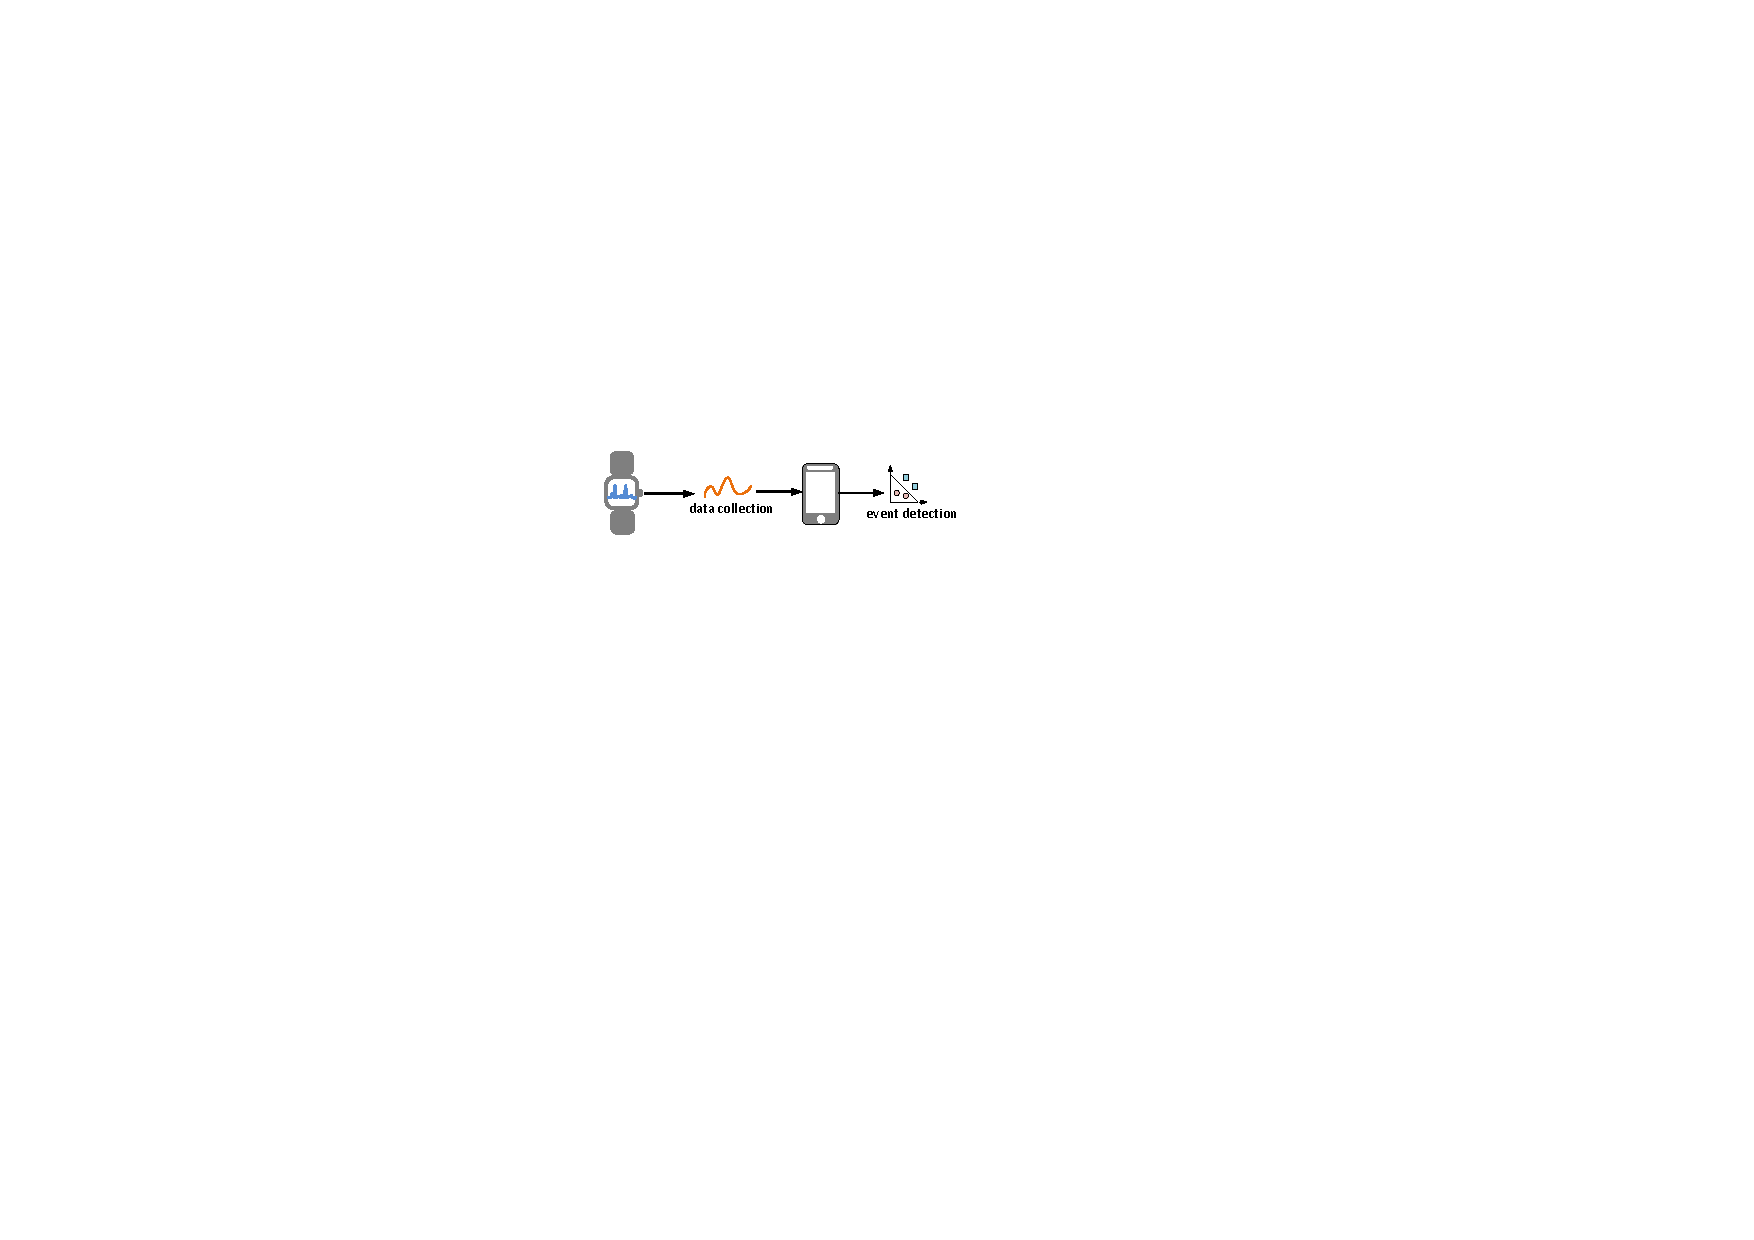
\includegraphics[width=0.7\textwidth]{figures/overviewd.pdf}\\
 %\caption{Overview of our 2-stage approach. Sleep data are collected through smartwatch sensors, which are then passed to be processedby a mobile app
%  to detect sleep events.}\label{fig:overview}
%\end{figure}

\systemname is a novel smartwatch-based sleep monitoring system that aims at estimating sleep quality and capturing rich information about
behaviours and events occurring during sleep. By capturing this information, \systemname can analyze potential reasons for sleep problems
and provide the user with suggestions on how to improve their sleep routine or sleep environment. To achieve its design goals, \systemname
exploits a wide range of sensors that are common on commercial off-the-shelf smarwatches: (i) accelerometer, gyroscope, and orientation
sensor are used to collect body and hand movements; (ii) microphone is used to measure level of ambient noise and to capture acoustic
events; and (iii) ambient light sensor is used to monitor illumination within the sleep environment. The different sensors and information
extracted from them are summarized in Table~\ref{tab:test}. In the following we discuss the different subcomponents of \systemname in
detail. 

%acoustic data, the ambient light sensor for illumination conditions, the orientation sensor for calibration. The collected data are
%transmitted to a smartphone via Bluetooth. We propose a set of new analysis and algorithms to effectively detect sleep events from the
%collected data. Table~\ref{tab:test} lists the set of sleep events supported by \systemname.
%Figure~\ref{fig:overview} depicts our 2-stage approach that involves collecting data using a smartwatch and sleep event detection using a
%smartphone. Sleep data are collected using smartwatches sensors. Our work

\begin{table}[t!]
 \caption{\label{tab:test}Sleep events targeted in this work}
 \centering
 \begin{tabular}{ll}
  %\toprule
  \toprule
  \textbf{Event}& \textbf{Type} \\
  \midrule
\rowcolor{Gray}  Sleep postures & Supine, Left lateral, Left lateral, Prone\\
 Hand positions & Head, Chest, Abdomen\\
\rowcolor{Gray} Body rollover & Count\\
 Micro body movements& Hand moving, Arm raising, Body trembling \\
\rowcolor{Gray} Acoustic events & Snore, Cough, Somniloquy  \\
 Illumination condition & Strong, Weak  \\
  \bottomrule
 %\hline
 \end{tabular}
\end{table}

%\begin{figure}[!thbp]
%\centering
%%\setlength{\belowcaptionskip}{-9pt}
%      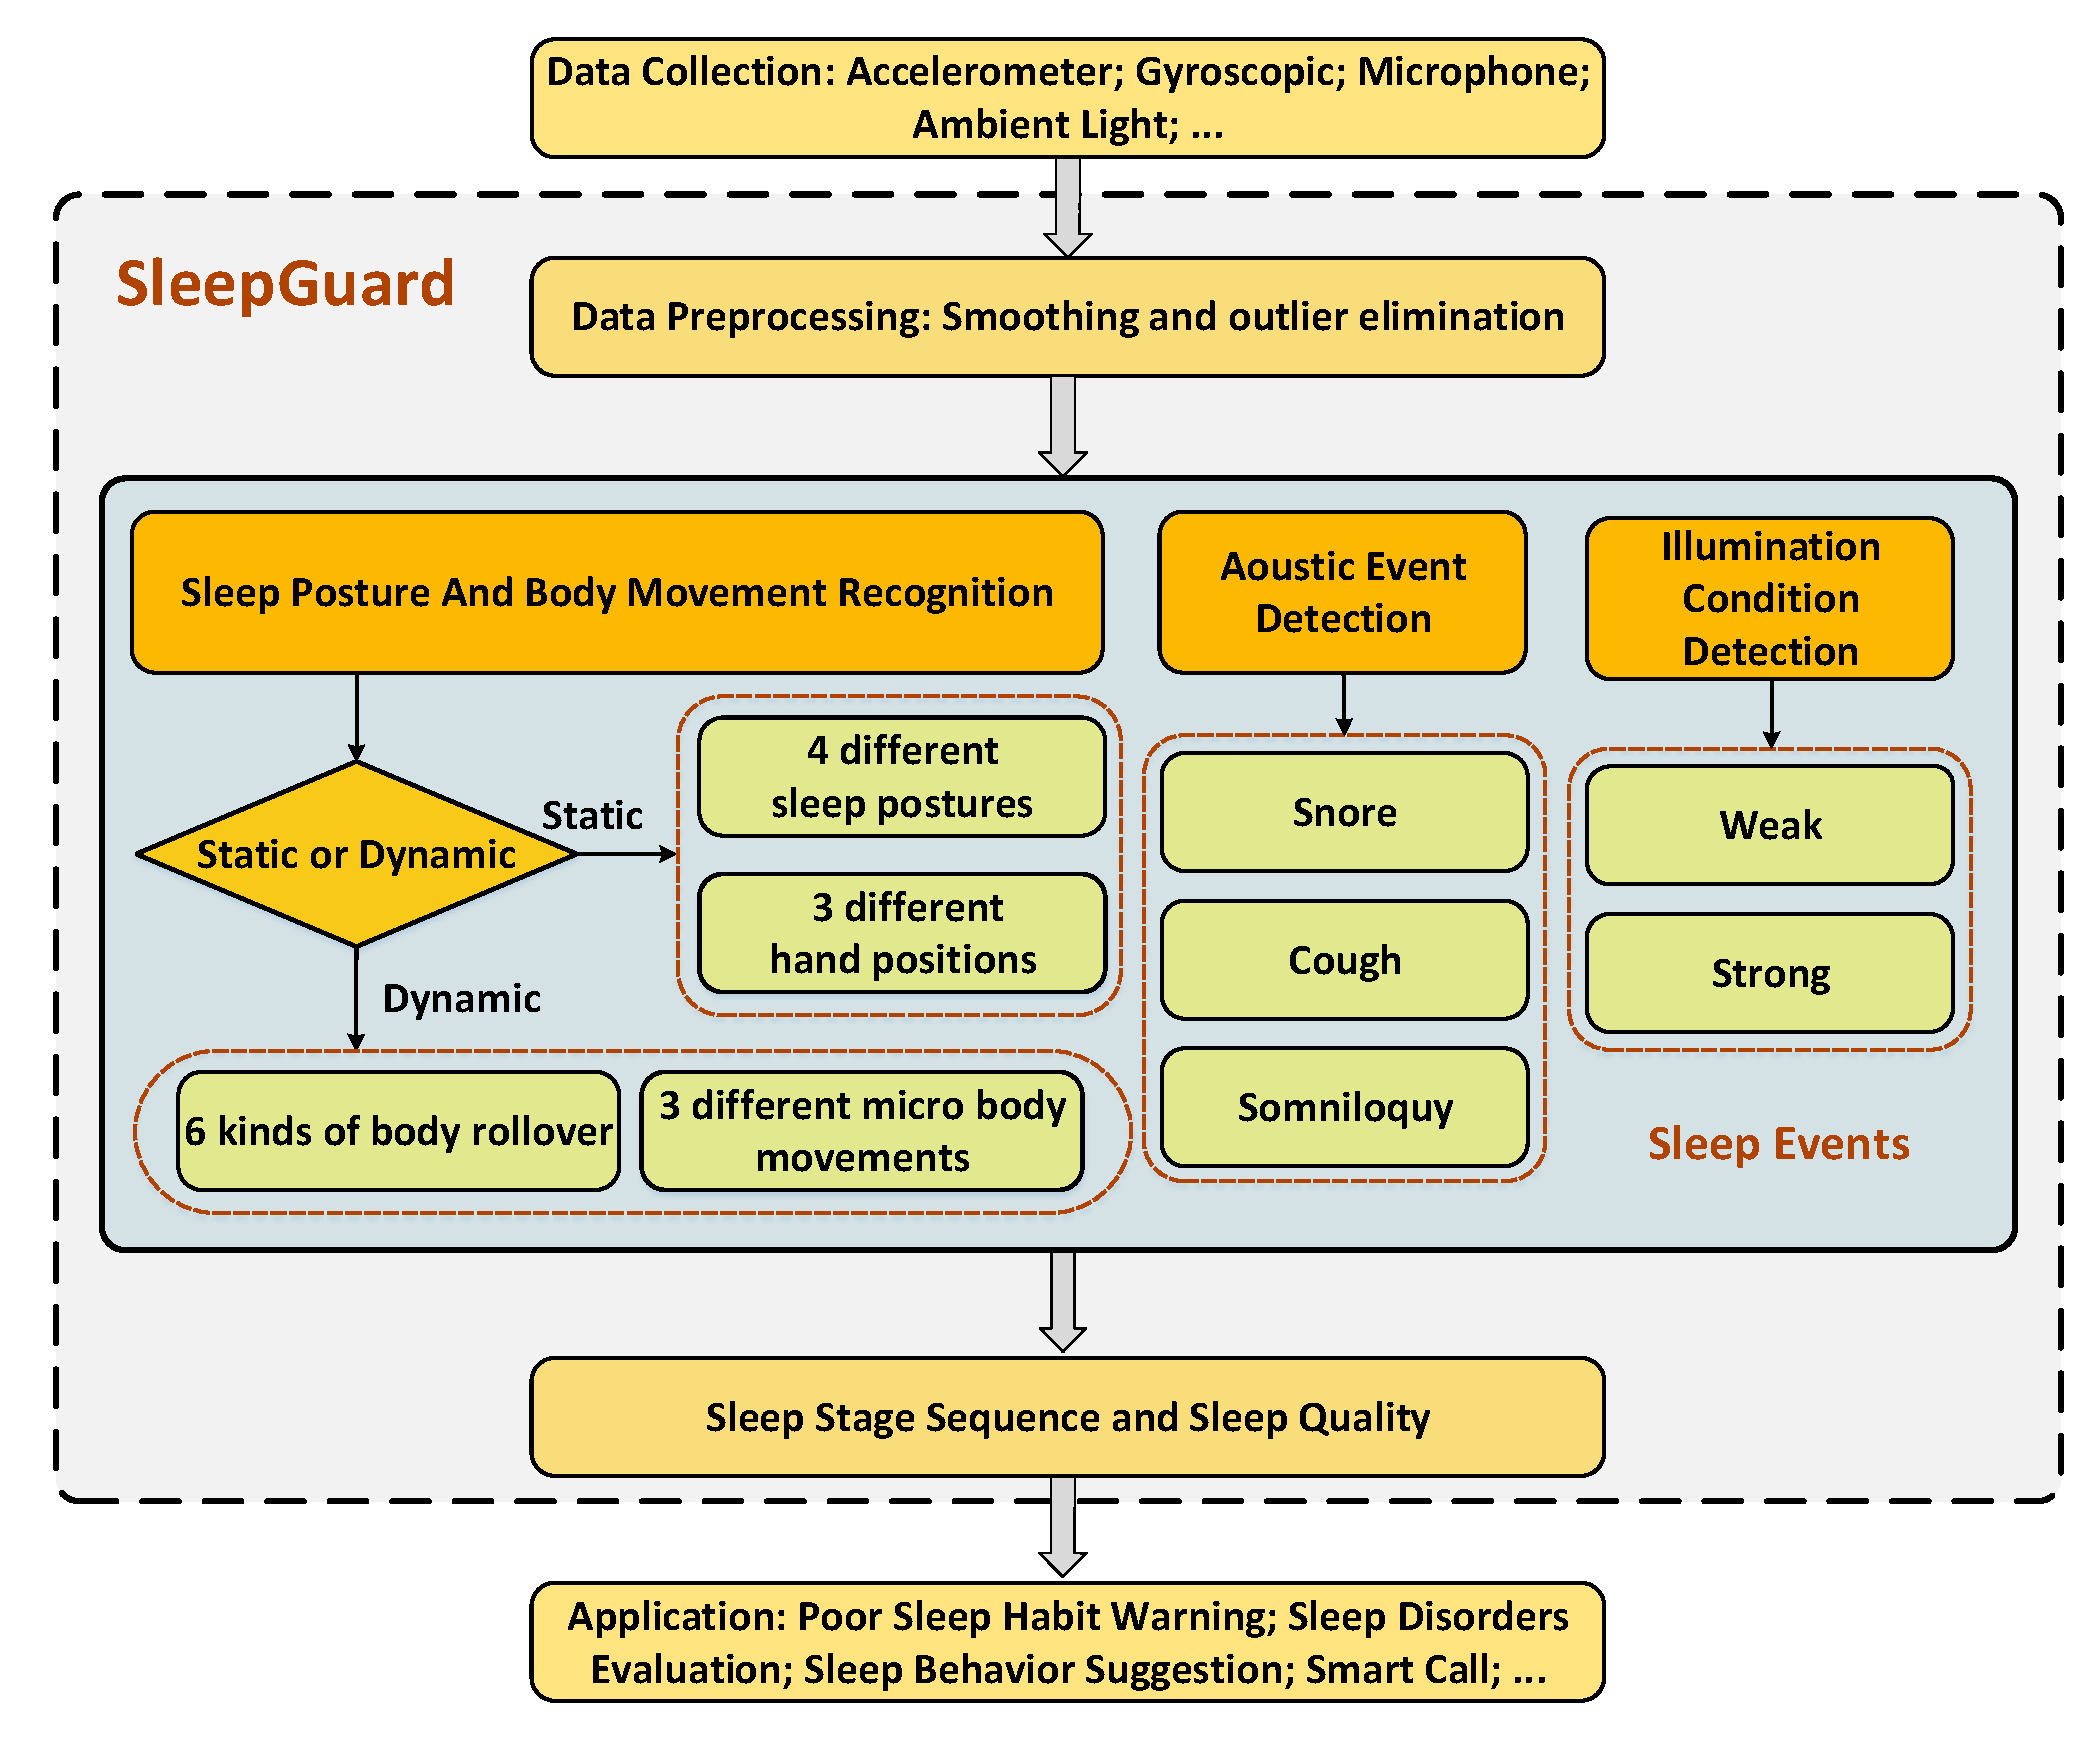
\includegraphics[width=0.97\linewidth]{Figures/SystemFlow.pdf}
%  \caption{System overview of {\systemname}.}\label{fig:overview}
%\end{figure}
%
%
%\begin{itemize}[itemsep=1mm,nolistsep]
%  \item {\textbf{Data Collection and Preprocessing.}} A variety of sensing data are related to sleep events include i) the accelerometer and the gyroscope about the body movement, ii) the microphone measured acoustic sound, iii) the ambient light sensor about the illumination condition, and iv) the orientation sensor with some auxiliary information. The data is collected every 30 ms on the smartwatch and transferred to the server (such as a smartphone) via Bluetooth. We use data smoothing and outlier elimination to reduce noise in the raw sensor readings.
%  \item \textbf{Sleep Event Detection.} A series of novel algorithms are developed to recognize different sleep events. In particular, some key insights are observed about different body postures, body rollovers, hand positions, micro body movements and acoustic events. Note that before identifying those events, {\systemname} first carries out a coarse-grained detection and judges whether the user is lying or not.  After that, we can estimate the user's bedtime. During the user is lying on the bed,  we regard that the user fell asleep if we do not detect a large movement within 20 minutes.
%  \item \textbf{{Sleep Pattern Report.}} Sleep Pattern Report. After we obtain the detected sleep events, we integrate them to the clock information, illumination condition, and then use the Hidden Markov Model to infer the sleep stages and evaluate sleep quality. Different from existing apps on the market, {\systemname} provides detailed procedure about the sleep report. The output of our system, for example, sleep postures and the position of user's hand could be used as input to build a broad range of sleeping quality and  heathy applications, such as poor sleep habit warning, the evaluation of insomnia, nightmare and sleep disorders. With the extensive experiments conducted, we conclude that {\systemname} exhibits a relatively high accuracy comparing to state-of-the-art systems.
%\end{itemize}


%\subsection{Feature Calculation and Selection}
%Appropriate  features  can  reflect  the  potential  information  underlying the  signals. The  features  used  in {\systemname} are shown in  Table \ref{Tab1}. To detect different sleep events, we use two main features. The first one is the movement related features, that are angle of inclination calculated by acceleration data and the angle of rotation calculated by gyroscopic data. Beyond that, to detect different sound events during sleep, we calculate the energy and zero-crossing rate of the sound signal.
%
%\begin{table}[!thbp]
%\centering
% \caption{Calculated Features}\label{Tab1}
%   \renewcommand\arraystretch{1.7}{\multirowsetup}{\centering}
%        \begin{tabular}{c|c|c}
%        \hline
%        {\bf{Data}}  &   {\bf{Feature}} &   {\bf{Formula}}\\
%         \hline
%        {$acc$} & {Tilt Angle}   & $ A_x =\arccos(\frac {acc_x}{acc}) $ \\
%        \hline
%        {$\omega$} &  {Rotation Angle}  & $ \theta = \int\omega $ \\
%        \hline
%        %\multirow{2} {0.1cm}
%        {Sound}  & Energy   &$ E=\sum\nolimits_{n=-\infty}^{\infty}|x^2(n)|$ \\
%         {$x(n)$}  & Zero-crossing  & $Z$ \\
%          \hline
%\end{tabular}
%\end{table}

\section{\systemname Sleep Monitoring Platform}\label{Sec:3design}

%\subsection{Overview of \systemname}

%\begin{figure}
%  \centering
  % Requires \usepackage{graphicx}
 % 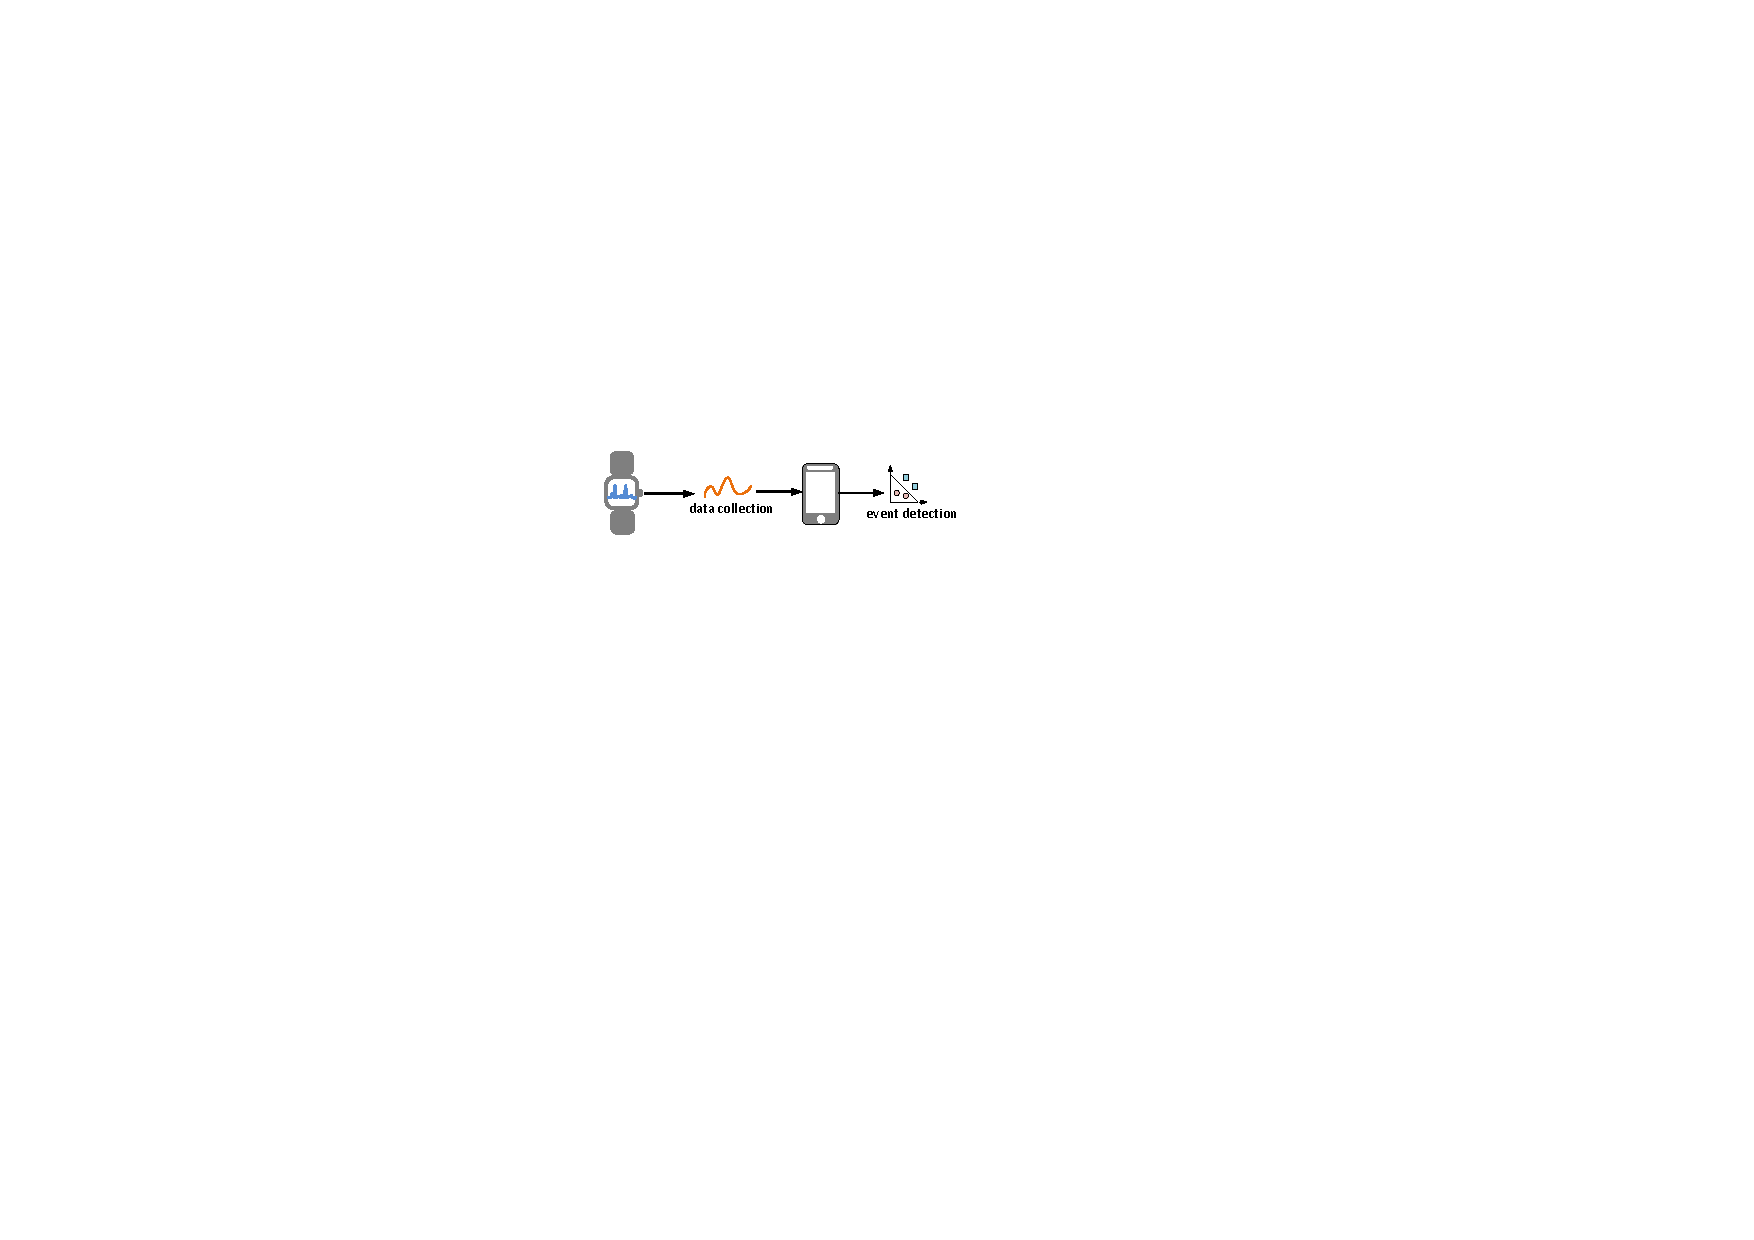
\includegraphics[width=0.7\textwidth]{figures/overviewd.pdf}\\
 %\caption{Overview of our 2-stage approach. Sleep data are collected through smartwatch sensors, which are then passed to be processedby a mobile app
%  to detect sleep events.}\label{fig:overview}
%\end{figure}

\systemname is a novel smartwatch-based sleep monitoring system that aims at estimating sleep quality and capturing rich information about
behaviours and events occurring during sleep. By capturing this information, \systemname can analyze potential reasons for sleep problems
and provide the user with suggestions on how to improve their sleep routine or sleep environment. To achieve its design goals, \systemname
exploits a wide range of sensors that are common on commercial off-the-shelf smarwatches: (i) accelerometer, gyroscope, and orientation
sensor are used to collect body and hand movements; (ii) microphone is used to measure level of ambient noise and to capture acoustic
events; and (iii) ambient light sensor is used to monitor illumination within the sleep environment. The different sensors and information
extracted from them are summarized in Table~\ref{tab:test}. In the following we discuss the different subcomponents of \systemname in
detail. 

%acoustic data, the ambient light sensor for illumination conditions, the orientation sensor for calibration. The collected data are
%transmitted to a smartphone via Bluetooth. We propose a set of new analysis and algorithms to effectively detect sleep events from the
%collected data. Table~\ref{tab:test} lists the set of sleep events supported by \systemname.
%Figure~\ref{fig:overview} depicts our 2-stage approach that involves collecting data using a smartwatch and sleep event detection using a
%smartphone. Sleep data are collected using smartwatches sensors. Our work

\begin{table}[t!]
 \caption{\label{tab:test}Sleep events targeted in this work}
 \centering
 \begin{tabular}{ll}
  %\toprule
  \toprule
  \textbf{Event}& \textbf{Type} \\
  \midrule
\rowcolor{Gray}  Sleep postures & Supine, Left lateral, Left lateral, Prone\\
 Hand positions & Head, Chest, Abdomen\\
\rowcolor{Gray} Body rollover & Count\\
 Micro body movements& Hand moving, Arm raising, Body trembling \\
\rowcolor{Gray} Acoustic events & Snore, Cough, Somniloquy  \\
 Illumination condition & Strong, Weak  \\
  \bottomrule
 %\hline
 \end{tabular}
\end{table}

%\begin{figure}[!thbp]
%\centering
%%\setlength{\belowcaptionskip}{-9pt}
%      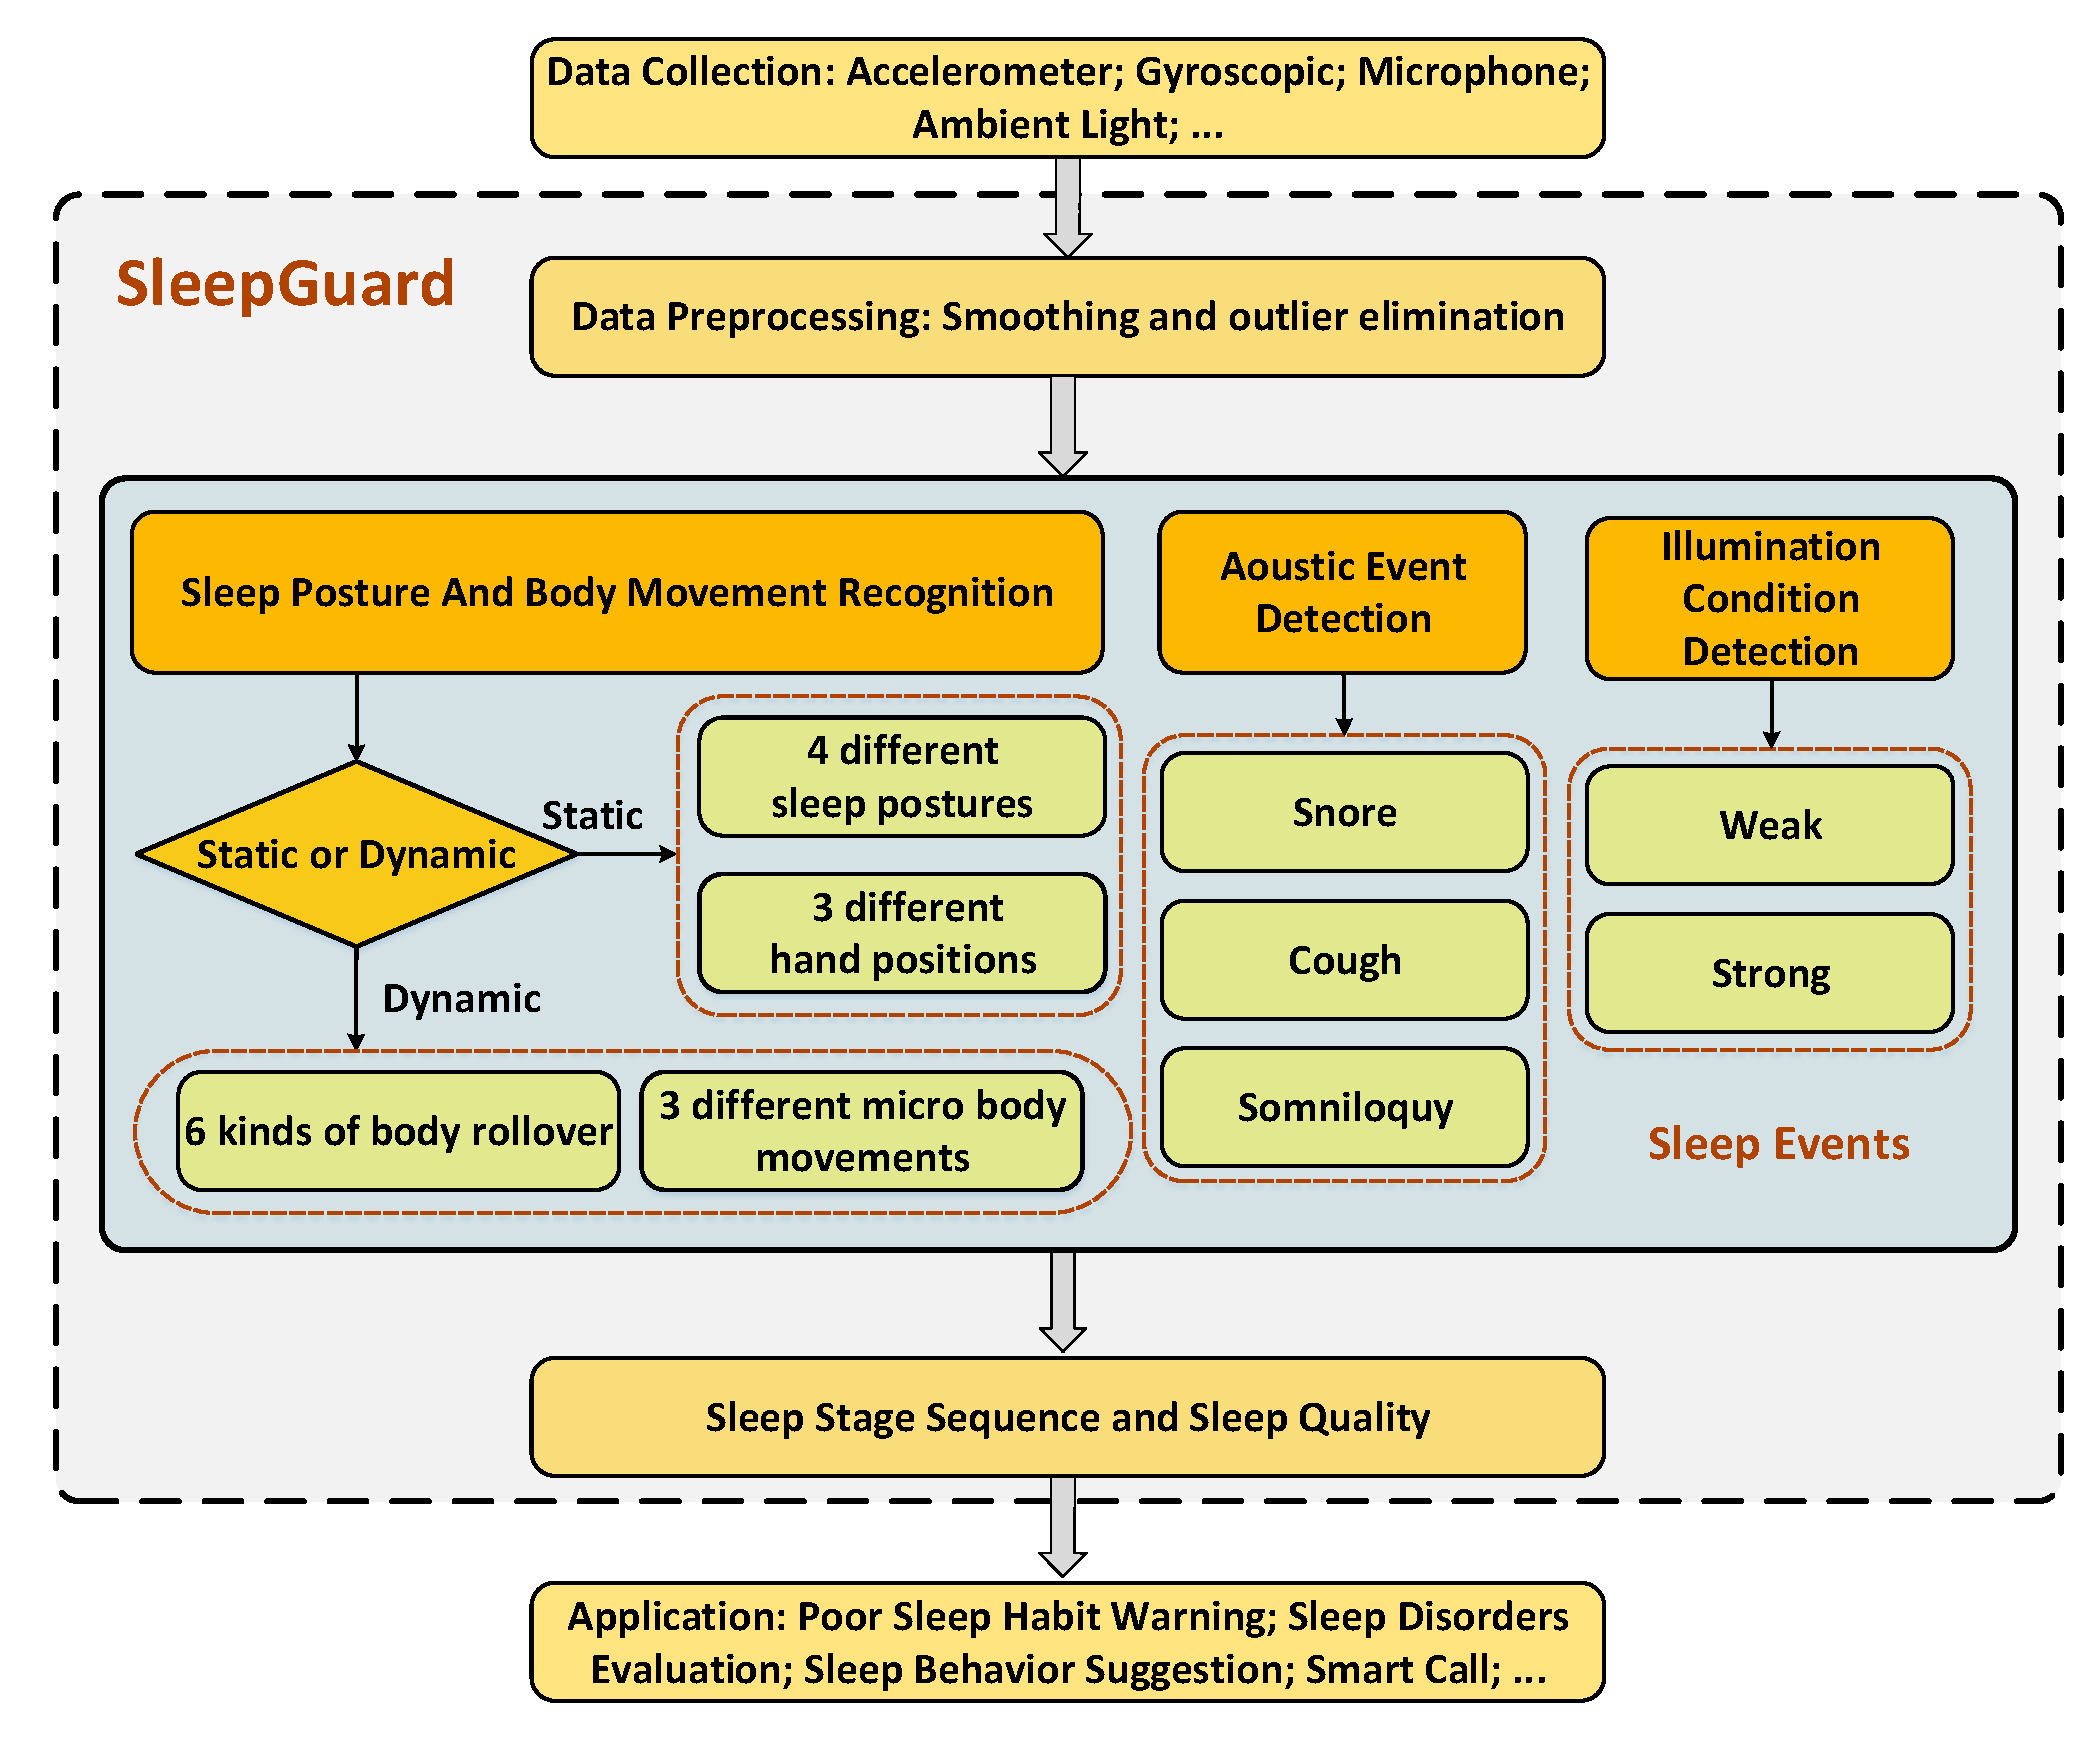
\includegraphics[width=0.97\linewidth]{Figures/SystemFlow.pdf}
%  \caption{System overview of {\systemname}.}\label{fig:overview}
%\end{figure}
%
%
%\begin{itemize}[itemsep=1mm,nolistsep]
%  \item {\textbf{Data Collection and Preprocessing.}} A variety of sensing data are related to sleep events include i) the accelerometer and the gyroscope about the body movement, ii) the microphone measured acoustic sound, iii) the ambient light sensor about the illumination condition, and iv) the orientation sensor with some auxiliary information. The data is collected every 30 ms on the smartwatch and transferred to the server (such as a smartphone) via Bluetooth. We use data smoothing and outlier elimination to reduce noise in the raw sensor readings.
%  \item \textbf{Sleep Event Detection.} A series of novel algorithms are developed to recognize different sleep events. In particular, some key insights are observed about different body postures, body rollovers, hand positions, micro body movements and acoustic events. Note that before identifying those events, {\systemname} first carries out a coarse-grained detection and judges whether the user is lying or not.  After that, we can estimate the user's bedtime. During the user is lying on the bed,  we regard that the user fell asleep if we do not detect a large movement within 20 minutes.
%  \item \textbf{{Sleep Pattern Report.}} Sleep Pattern Report. After we obtain the detected sleep events, we integrate them to the clock information, illumination condition, and then use the Hidden Markov Model to infer the sleep stages and evaluate sleep quality. Different from existing apps on the market, {\systemname} provides detailed procedure about the sleep report. The output of our system, for example, sleep postures and the position of user's hand could be used as input to build a broad range of sleeping quality and  heathy applications, such as poor sleep habit warning, the evaluation of insomnia, nightmare and sleep disorders. With the extensive experiments conducted, we conclude that {\systemname} exhibits a relatively high accuracy comparing to state-of-the-art systems.
%\end{itemize}


%\subsection{Feature Calculation and Selection}
%Appropriate  features  can  reflect  the  potential  information  underlying the  signals. The  features  used  in {\systemname} are shown in  Table \ref{Tab1}. To detect different sleep events, we use two main features. The first one is the movement related features, that are angle of inclination calculated by acceleration data and the angle of rotation calculated by gyroscopic data. Beyond that, to detect different sound events during sleep, we calculate the energy and zero-crossing rate of the sound signal.
%
%\begin{table}[!thbp]
%\centering
% \caption{Calculated Features}\label{Tab1}
%   \renewcommand\arraystretch{1.7}{\multirowsetup}{\centering}
%        \begin{tabular}{c|c|c}
%        \hline
%        {\bf{Data}}  &   {\bf{Feature}} &   {\bf{Formula}}\\
%         \hline
%        {$acc$} & {Tilt Angle}   & $ A_x =\arccos(\frac {acc_x}{acc}) $ \\
%        \hline
%        {$\omega$} &  {Rotation Angle}  & $ \theta = \int\omega $ \\
%        \hline
%        %\multirow{2} {0.1cm}
%        {Sound}  & Energy   &$ E=\sum\nolimits_{n=-\infty}^{\infty}|x^2(n)|$ \\
%         {$x(n)$}  & Zero-crossing  & $Z$ \\
%          \hline
%\end{tabular}
%\end{table}




\begin{figure*}
	\centering
	\begin{minipage}[t]{.33\textwidth}
		\centering
		  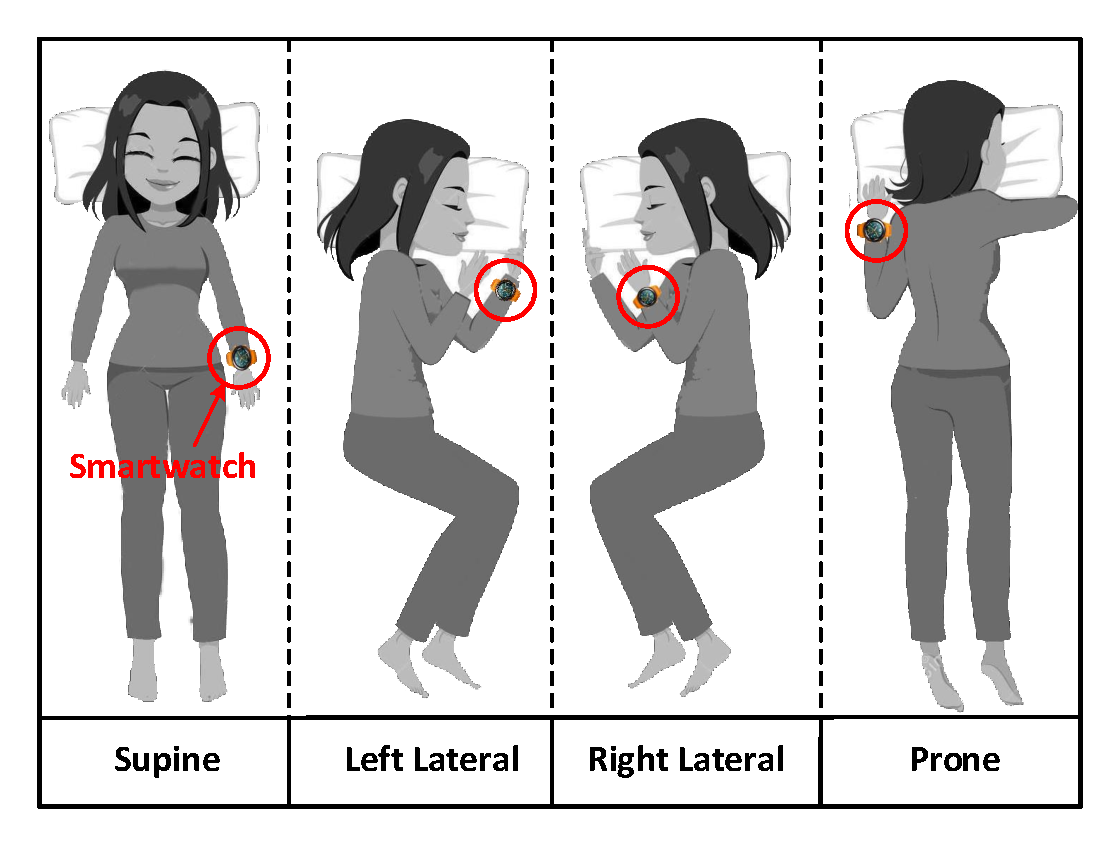
\includegraphics[width=4.7cm,height=3.7cm]{Figures/BodyPosture.pdf}
		\caption{Four sleep body postures.}
		\label{fig:BodyPosture}
	\end{minipage}%
	\begin{minipage}[t]{.33\textwidth}
		\centering
		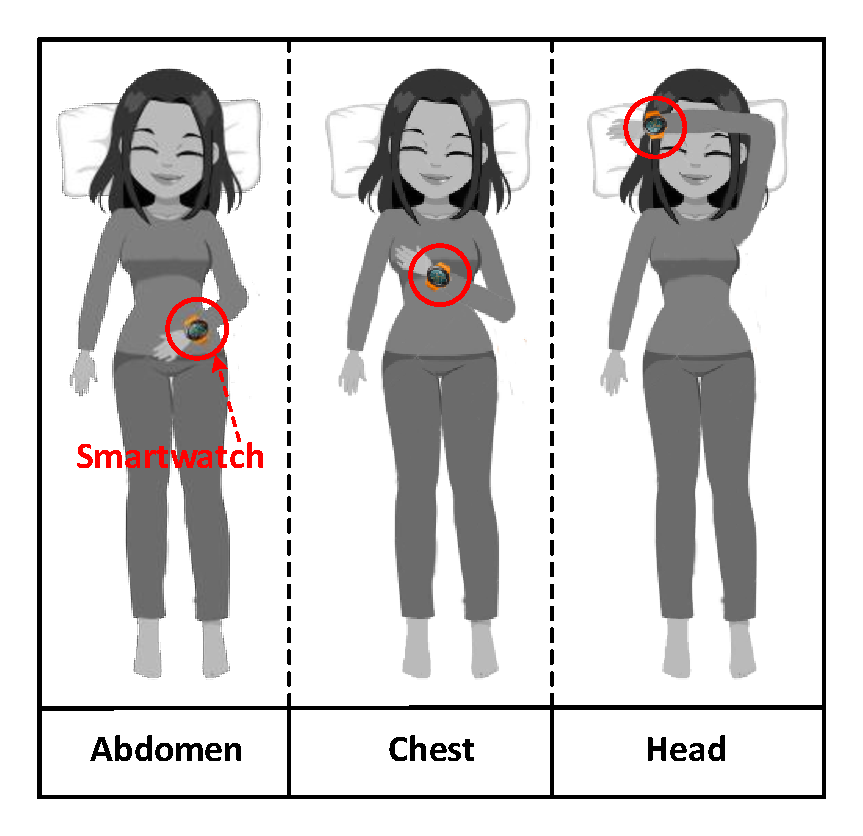
\includegraphics[width=4.1cm,height=3.4cm]{Figures/HandPosition.pdf}
		\caption{Three hand positions.}
		\label{fig:HandPosition}		
	\end{minipage}
\begin{minipage}[t]{.33\textwidth}
		\centering
	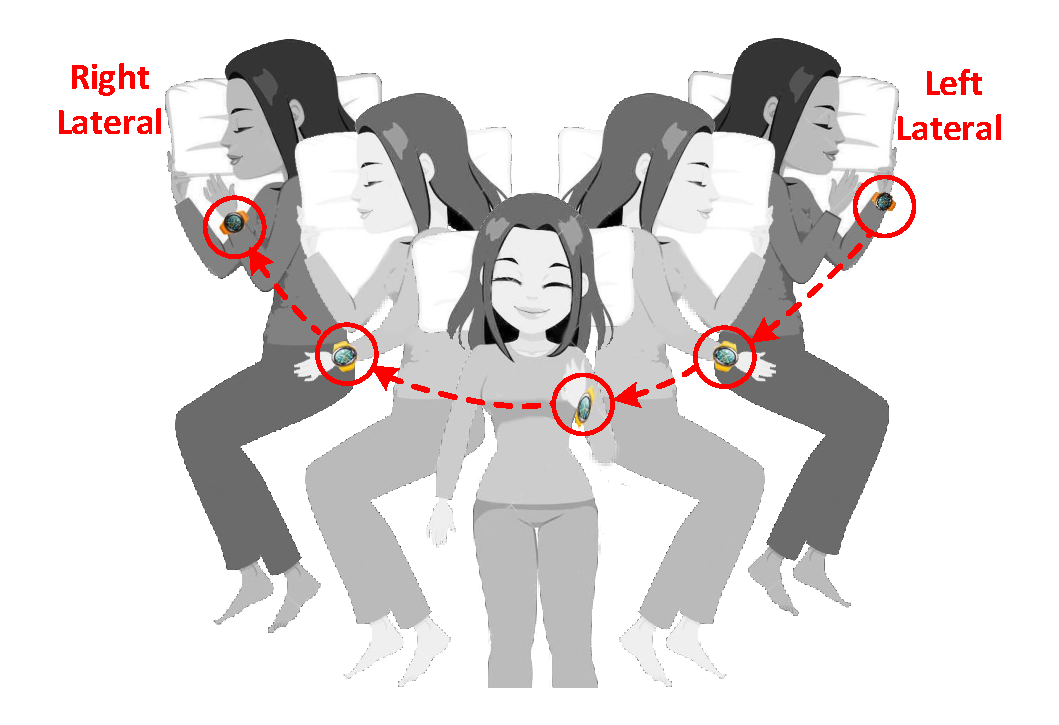
\includegraphics[width=4.7cm,height=3.7cm]{Figures/BodyRollover.pdf}
	\caption{Body rollover from the left side to the right side.}
	\label{fig:BodyRollover}
\end{minipage}
\end{figure*}




\subsection{Detecting Sleep Postures and Movements}

One's sleeping position, referred to as {\em sleep posture}, and the extent of body movements are important factors in determining
overall sleep quality. Suboptimal posture has been shown to affect the severity of sleep disorders and is widely used in medical diagnoses
to analyse effects of sleep disorders~\cite{oksenberg1998effect,eiseman2012impact} while having a good sleep posture has been shown to
correlate with subjective assessments of sleep quality~\cite{dekoninck83sleep}. Similarly, high degree of body movements during sleep
likely reflects restlessness, which results in poor sleep quality. {\systemname} uses motion sensors (accelerometer, gyroscope, and
orientation sensor) to capture user's sleep posture and habits. In the following we detail the techniques we use for capturing the body
posture and movements.  {\systemname}, currently supports the 4 basic sleep postures (see Fig.~\ref{fig:BodyPosture}); 3 hand positions
(see Fig.~\ref{fig:HandPosition}); 6 types of body rollovers (see Fig.~\ref{fig:BodyRollover} for an example); and 3 types of body micro
movements. %These events comprehensively and highly relate to the sleep stages and quality.


\subsubsection{Sleep Posture Detection}
\label{sec:sleeppdet}

Dreaming and sleep quality are associated with underlying brain functions, which in turn are affected by body posture~\cite{posture2004}.
Sleep posture also varies across individuals and should fit personal and physical needs of the individual~\cite{posture2016,posture2017}.
For example, sleeping in a prone position is unsuitable for people with ailments, such as heart disease or high blood pressure. On the
other hand, people can \nt{unconsciously} avoid postures that would be beneficial for health and sleep quality~\cite{posture2015}. Having an
effective way to detect current posture and track changes in it would thus be essential for estimating overall sleep quality, and
avoiding potential harm. \nt{\systemname captures four basic sleep postures: supine, left lateral, right lateral, and prone. These are
illustrated in} Fig.~\ref{fig:BodyPosture}. Detecting these postures using a single wrist sensor, however, is non-trivial because the
sensor cannot accurately track movement of the entire body. To accomplish posture detection, we observe that the arm position strongly correlates \nt{with} sleep posture, i.e.,
the arm is typically located in a specific, stable location for a given posture. This  suggests that we can first identify the user's arm position and the {\em time the position is approximately stable, which can then be mapped into} a sleep posture. Later in this paper,
we show that our approach \nt{achieves} high accuracy in identifying sleep postures.




%\textcolor{blue}{As we all know, it is very difficult to use only a smartwatch to describe
%the posture of the entire body, but we found a key basis for sleeping posture detection through observation and a pilot (see Sec. 3.1).}
%The key intuition for distinguishing between these postures is that arms have common and (reasonably) stable positions in each posture.
%\textcolor{blue}{Thus, we can build a mapping between the user's arms position and sleeping postures and identify the user's posture by
%identifying periods where the hand is in a position that correlates with a specific posture.} The basic idea is similar to the posture
%recognition used in~\cite{sleepmonitor}, but we use an additional step to improve the accuracy of distinguishing between supine and prone
%positions.

To separate sleep postures, {\systemname} considers a set of feasible hand positions for each posture. \nt{In the supine position, we assume the user's hand to be on the left side of the body, on the abdomen, on the chest or on the head; in the left and right lateral positions we assume the hand to be close to the pillow, on the chest or on the waist; and, finally, in the prone position we assume the user's hand is on the side of the head or above his/her head.} These positions were selected based on a pilot carried out in our test environment (see Sec.~\ref{sec:expsetup}). Fig.~\ref{fig:BodyPosture} shows one possible hand position for each of the postures.

\begin{figure}
	\centering
	\subfigure[Supine]{
		\label{fig:Supine}
		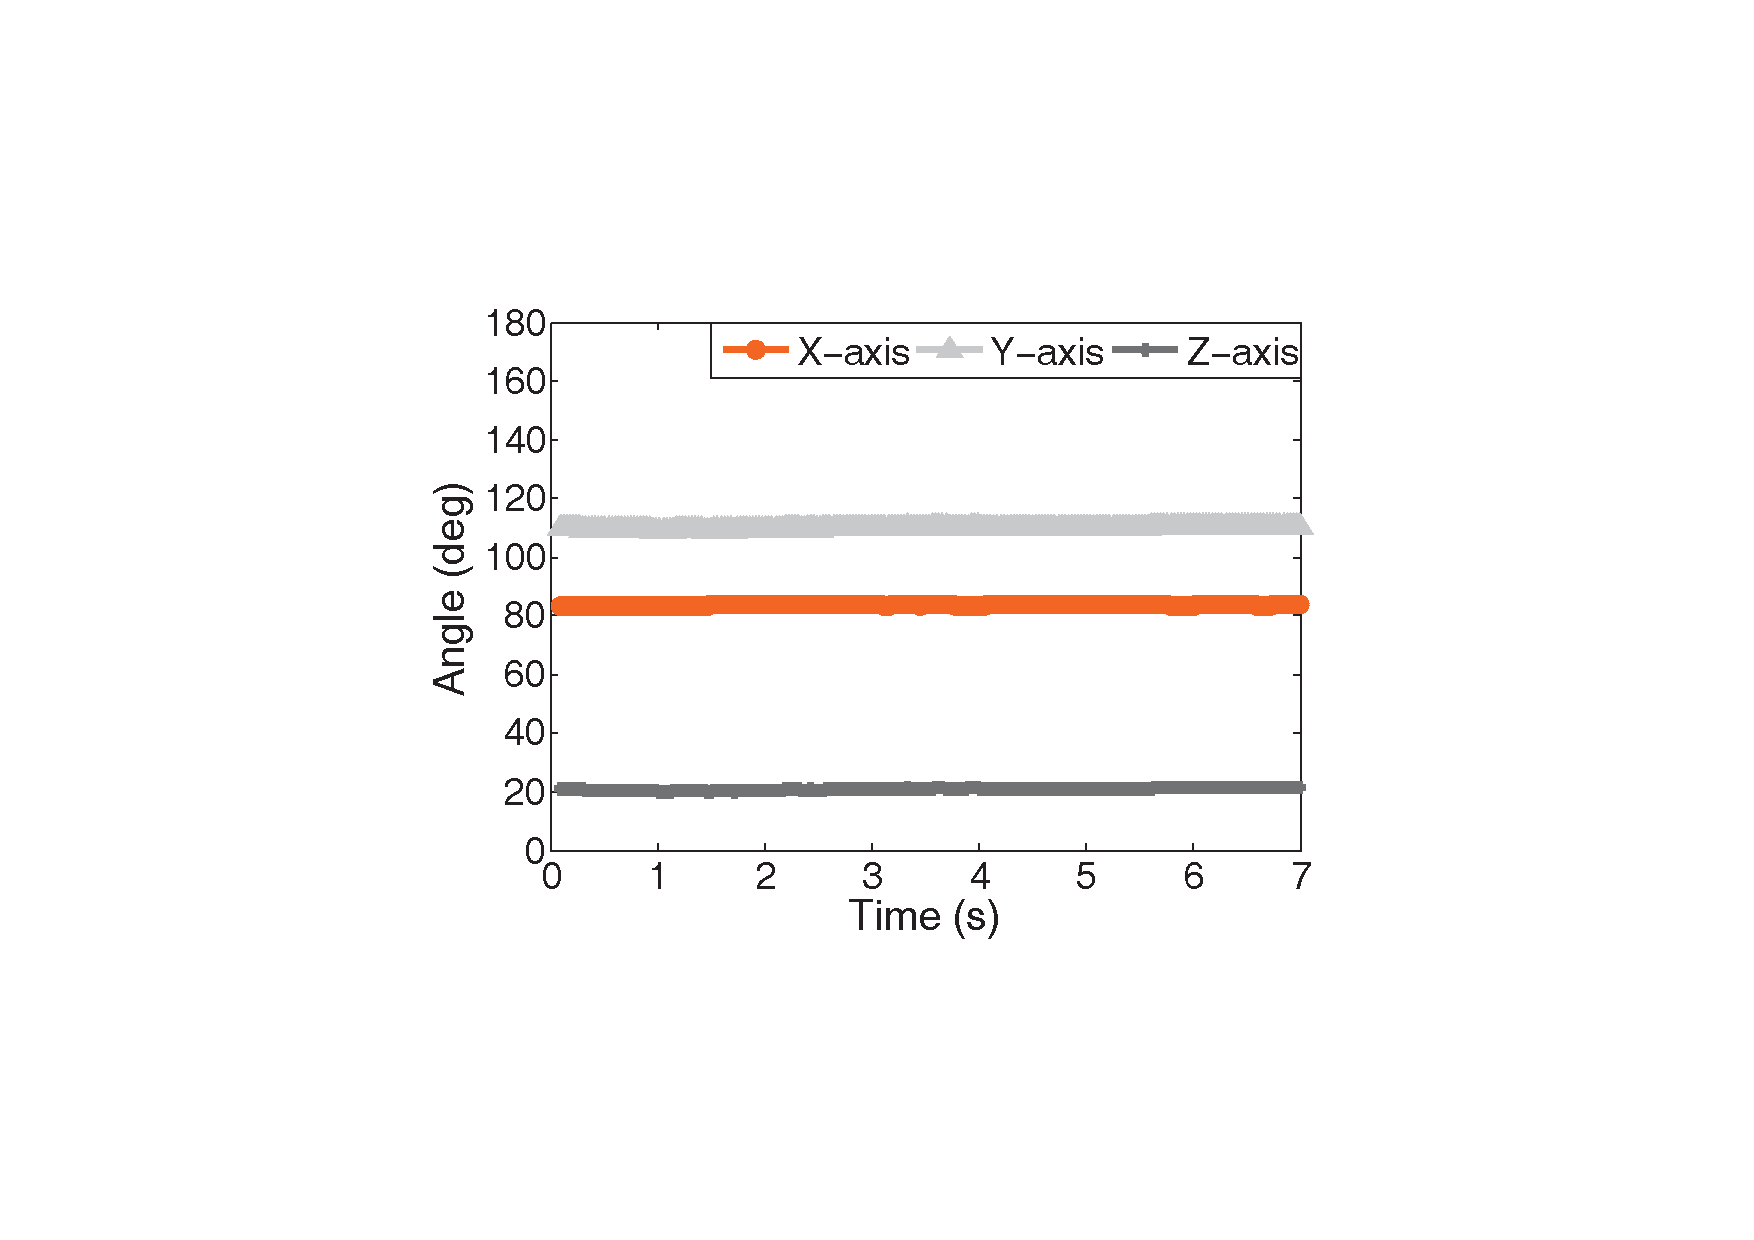
\includegraphics[width=0.24\linewidth]{Figures/Supine.pdf}}
	\hfill
	\subfigure[Left Lateral]{
		\label{fig:LeftLateral}
		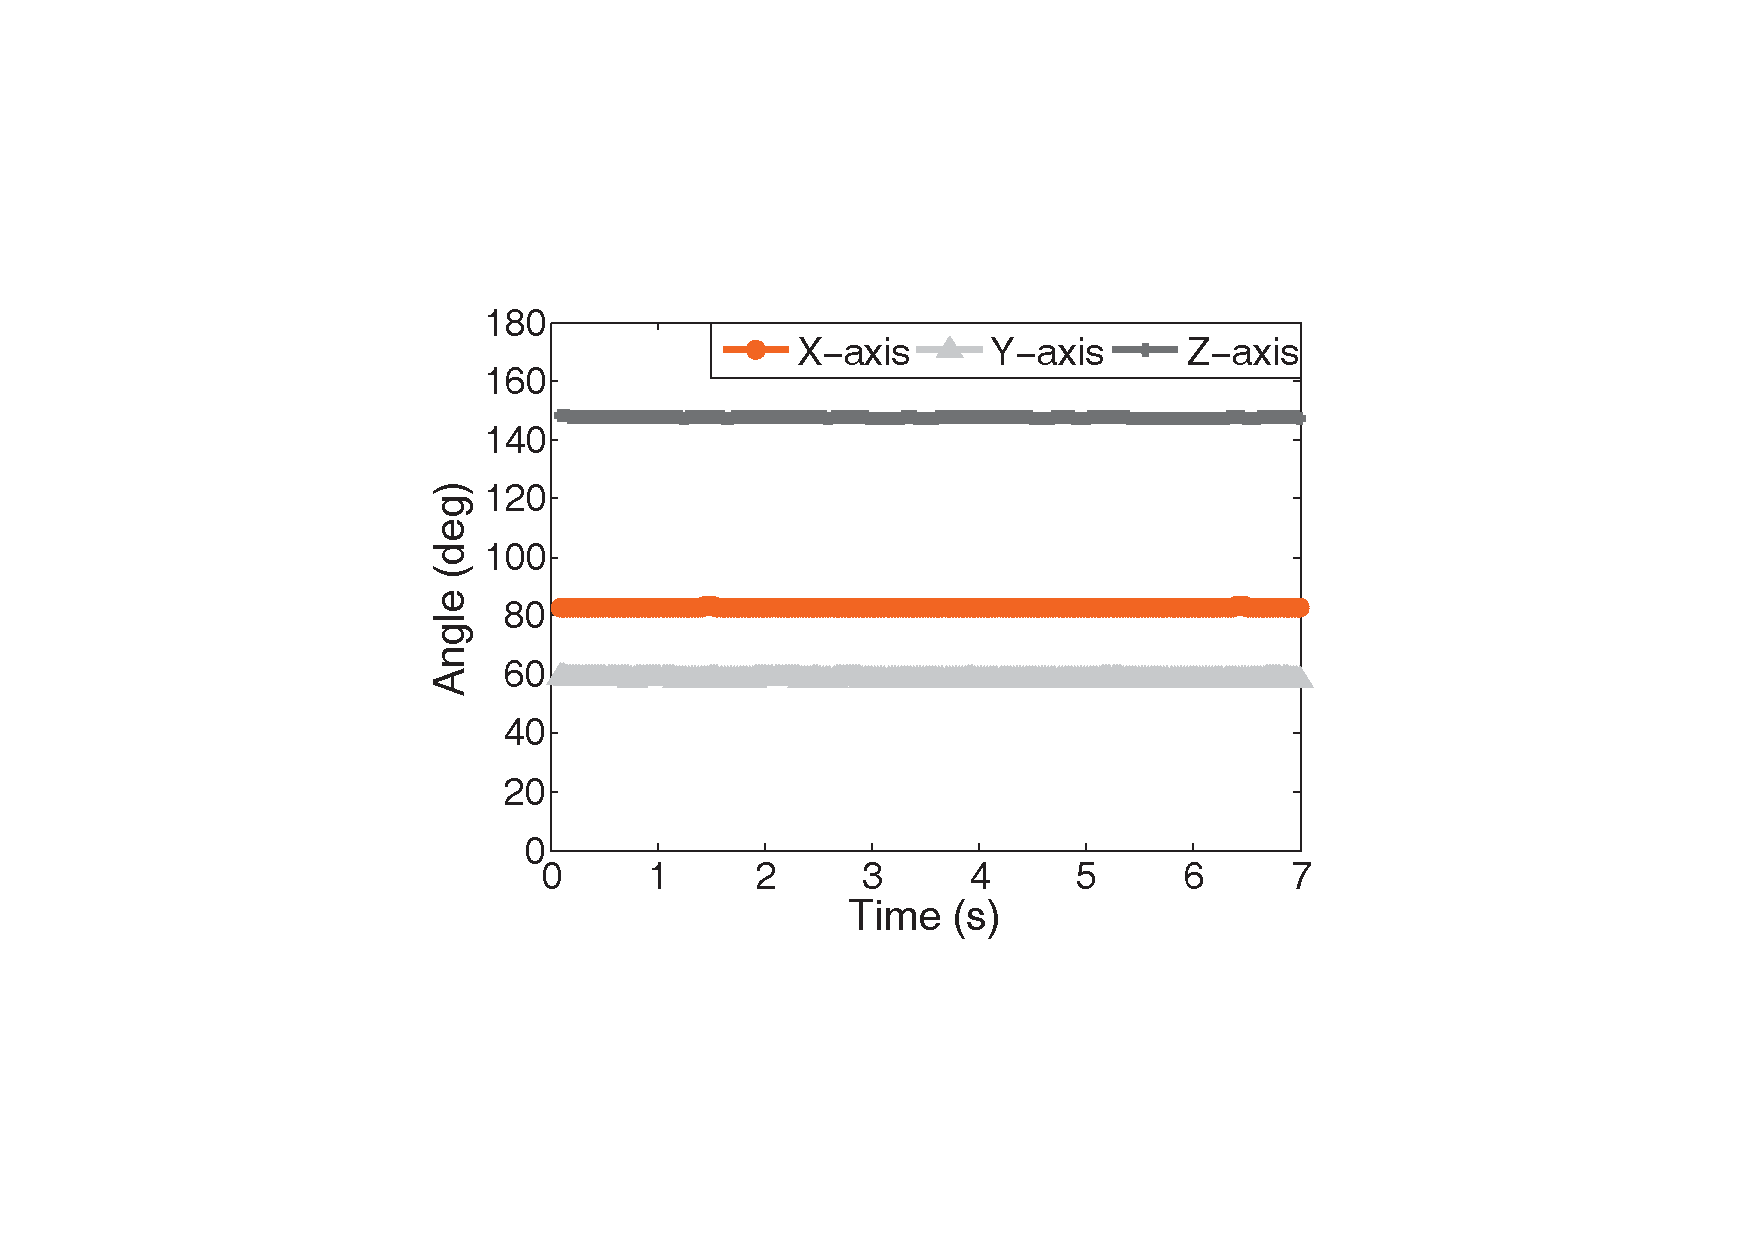
\includegraphics[width=0.24\linewidth]{Figures/LeftLateral.pdf}}
	\subfigure[Right Lateral]{
		\label{fig:RightLateral}
		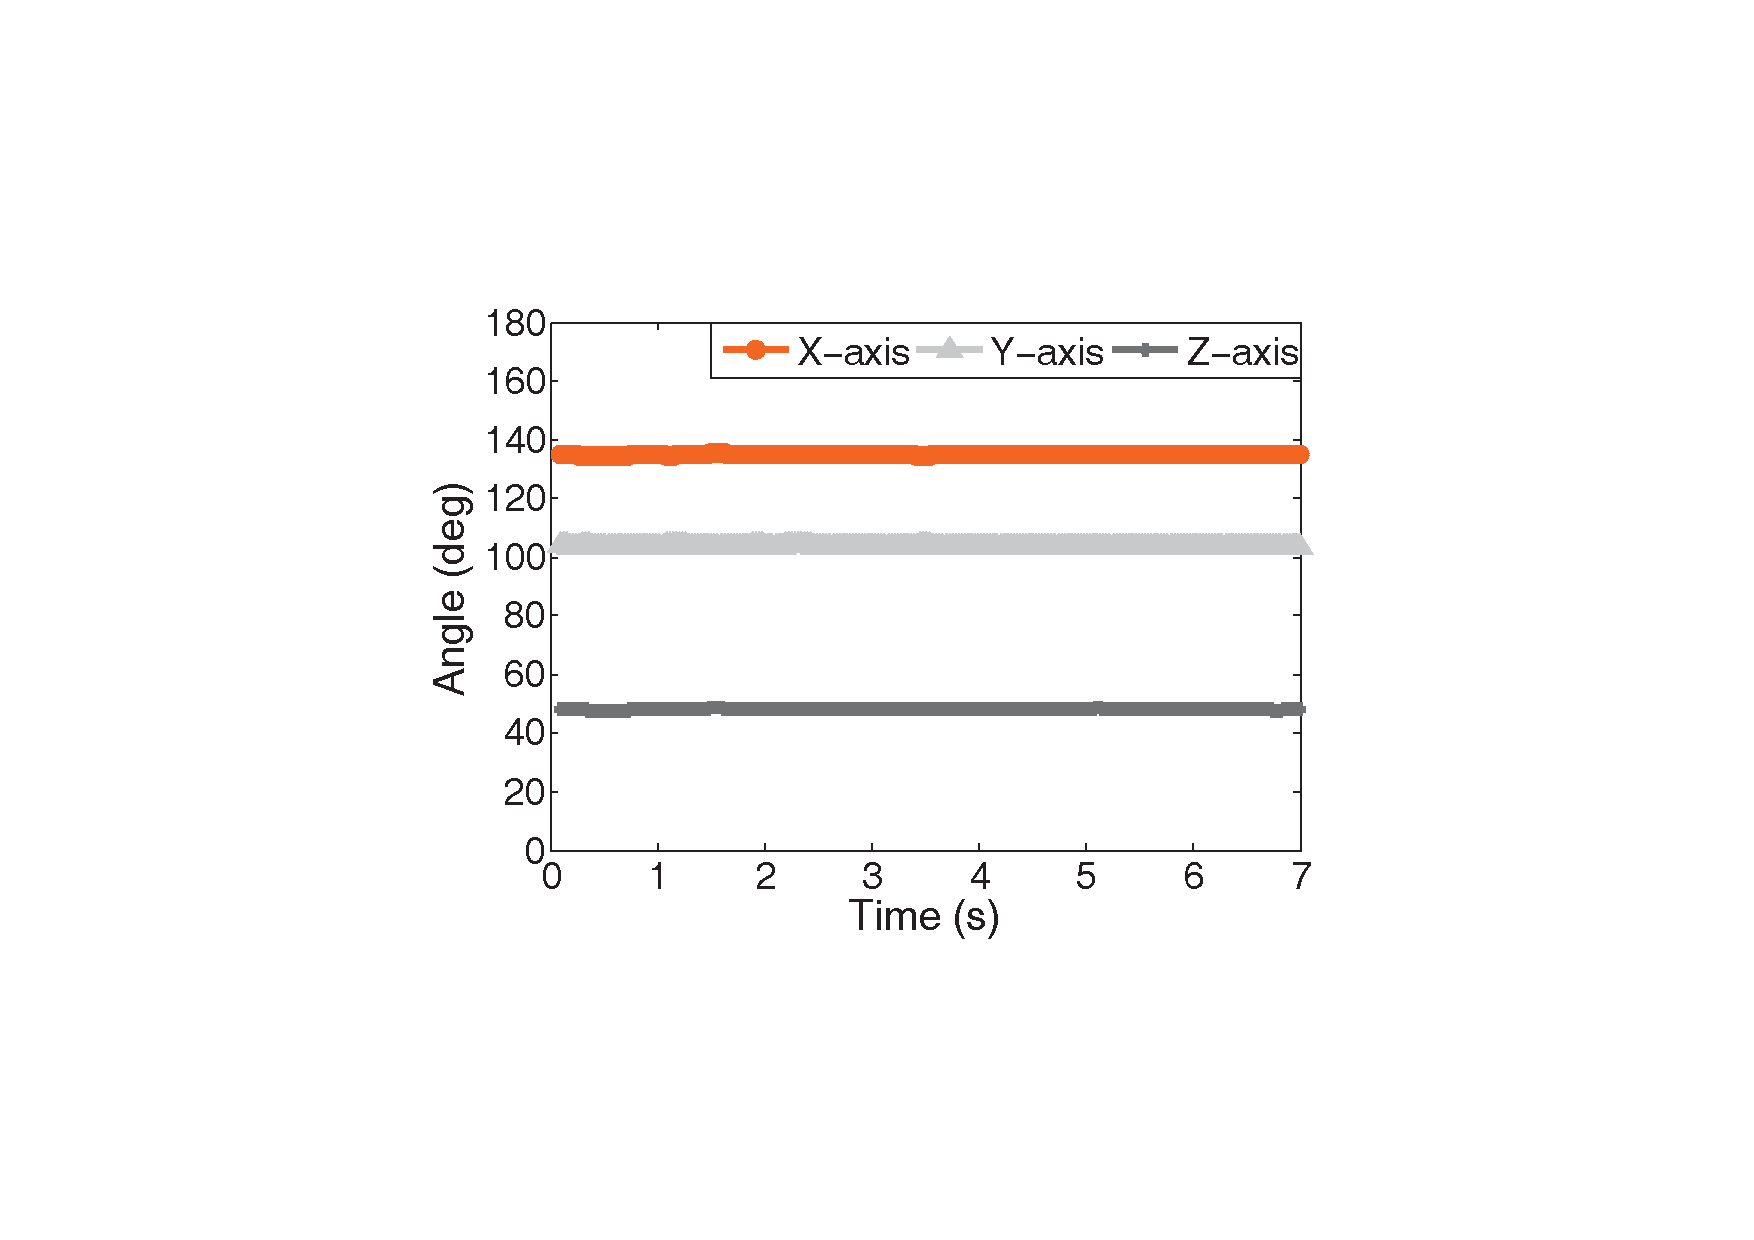
\includegraphics[width=0.24\linewidth]{Figures/RightLateral.pdf}}
	%\hspace{1in}
	\hfill
	\subfigure[Prone]{
		\label{fig:Prone}
		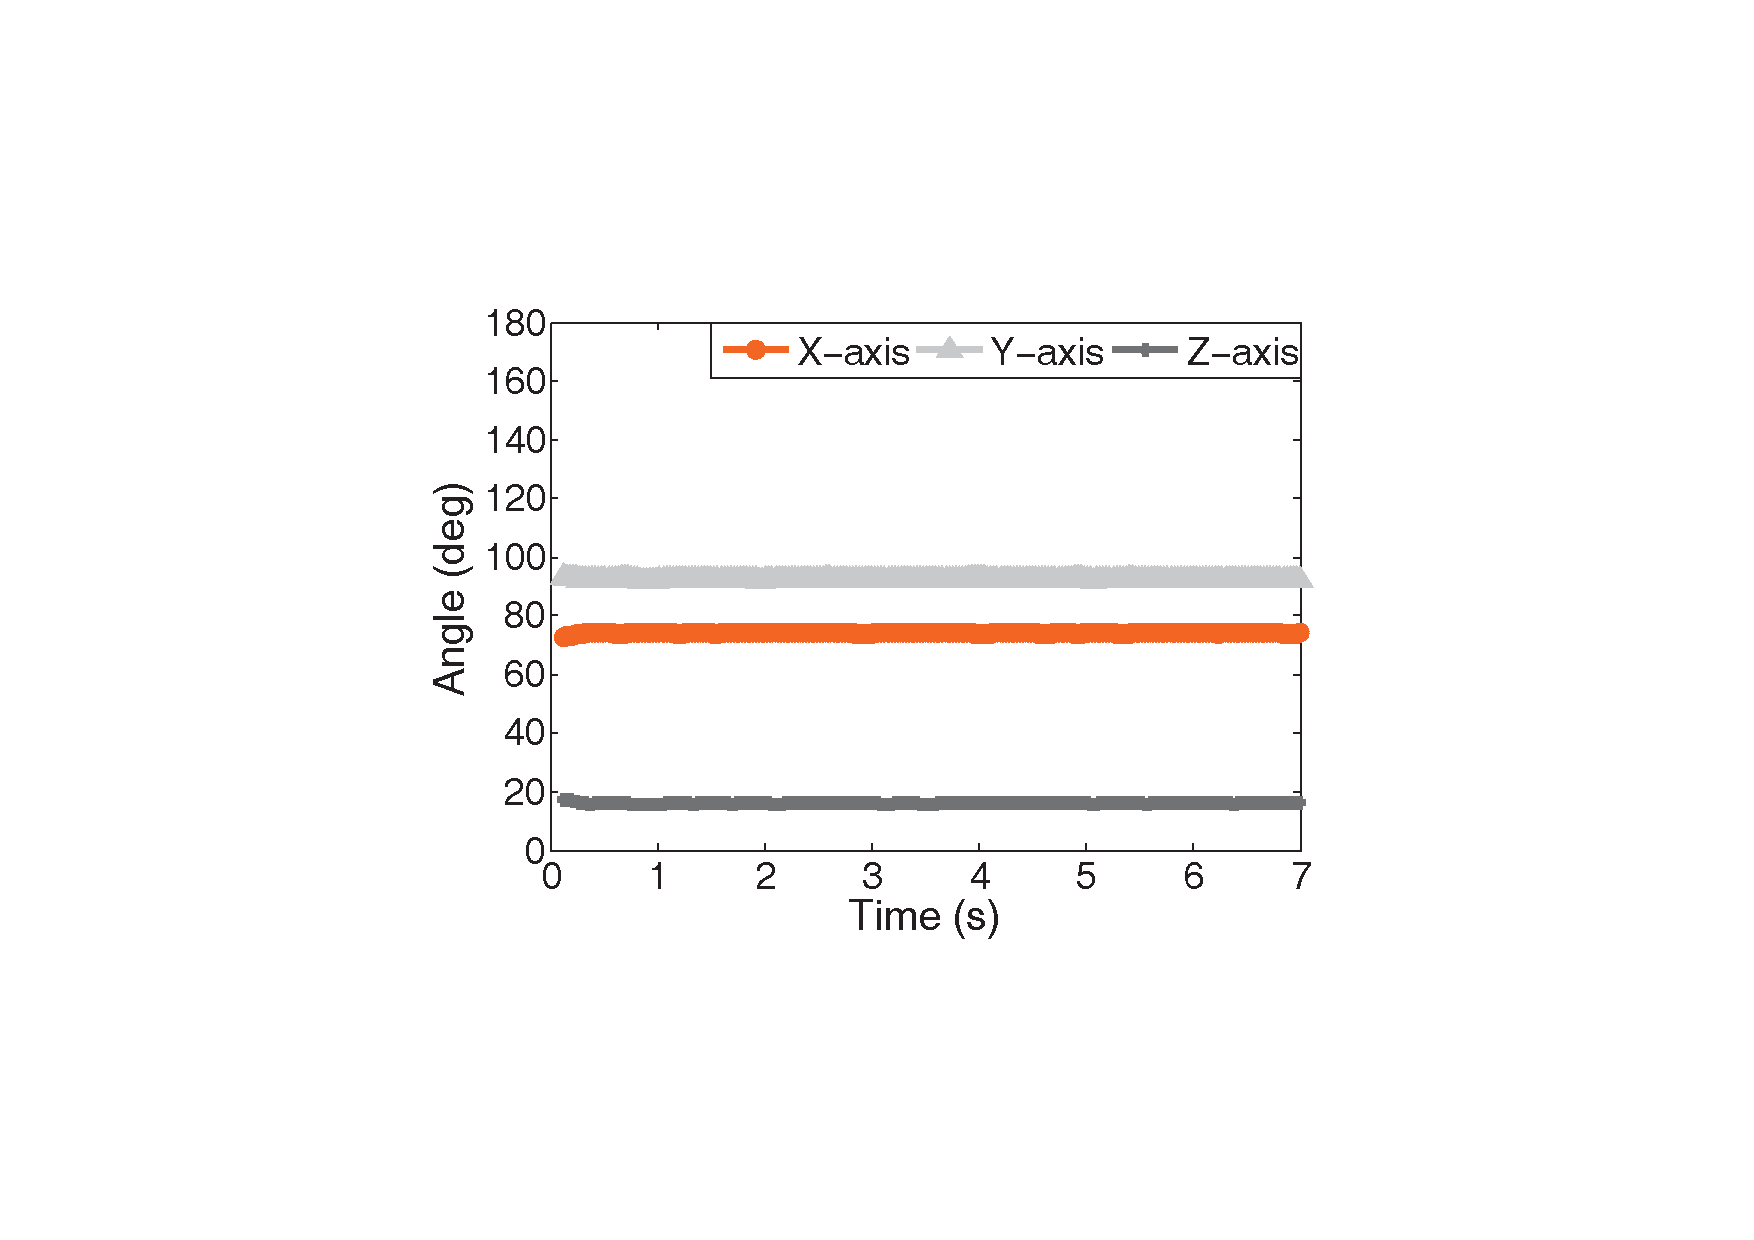
\includegraphics[width=0.24\linewidth]{Figures/Prone.pdf}}
	\caption{The tilt angle characteristics of four body postures.}
	\label{fig:posture}
\end{figure}

%e use a supervised classifier to  And then we use a supervised learning method to create a sleep posture profile. Specifically, we collect training data to create a mapping (i.e., angle mapping) between the angles and the arm under different positions.

% We use a K-nearest
%neighbour (KNN) classifier, where $k$ is set to 1,  to determine which of the target postures a input feature vector %corresponds
%to.


%each of the profiles across the three dimensional to find which
%profile is closest to the input values.

% To determine which posture an input feature corresponds to, we find which of
%the four posture profiles (i.e., tilt angle values in three dimensions) is closest to the input data. The posture profiles used for this
%task are collected from our pilot study involved 10 users who are different from the ones took part in our evaluation. To identify which of
%he postures the data collected within a time window corresponds to, we average all the calculate tilt angle values of that window in each
%dimension.


Similarly to SleepMonitor~\cite{sleepmonitor}, we use \nt{three dimensional tilt angles} to detect postures. To identify \nt{which posture data collected within a time window corresponds to}, we average all the calculated tilt angle values of that window in each dimension. We then calculate the Euclidean distance of the input values to a set of posture profiles, which are based on measurements collected in a pilot study that involved 10 users (see Sec.~\ref{sec:trainingdata}). We then use the body posture associated with the nearest neighbor as the detection outcome. Fig.~\ref{fig:posture} shows the angle values of the four sleep postures targeted in this work. \nt{We can observe clear differences in the tilt angles of the three axes}. The sleep posture thus can be inferred based on the position of the smartwatch and the created
angle mapping. However, a limitation of this approach is that the hand positions during supine and prone postures \nt{can be} similar when the hand
is located on the side of the head (Fig. \ref{fig:Supine} and \ref{fig:Prone}), thus the classification accuracy will be affected.

To improve detection accuracy between supine and prone postures, \systemname integrates orientation data as auxiliary feature. This is \nt{motivated by the observation that hand directions differ in supine and prone positions}. When the result of the previous step is prone or supine and hand is detected to be located next to the body, we combine the tilt angle with three axes data obtained from the direction sensor as a new feature, and classify these postures using a template-based distance matching approach. Specifically, we return the position corresponding to the template with minimum Euclidean distance with current sensor measurements as the user's posture. %Note that when we use the direction sensor, we must limit the pillow orientation remaining unchanged (in the experiment our pillow is placed on the north). In fact, this assumption can be easily satisfied since most people usually have fixed sleep directions.


\subsubsection{Hand Position Recognition\label{sec:handpr}}

Hand position during sleep can disclose potential health problems, and an improper hand position can even result in health issues~
\cite{position2014}. For instance, placing the hand on the abdomen may indicate discomfort whereas placing the hand on the chest can
increase the likelihood of nightmares due to long-term pressure on the heart. Similarly, placing the hand on the head can put excess
pressure on shoulder nerves and cause arm pain as blood flow is restricted. This can lead to eventual nerve damage, with symptoms including
a tingling sensation and numbness \cite{position2014}.


{\systemname} is designed to recognize three common hand positions -- if the hand is placed on the abdomen, chest or head when the user is
in the supine posture, as shown in Fig. \ref{fig:HandPosition}. We have chosen these three hand positions because there are found to be the
most common and representative positions in our pilot study (Sec.~\ref{sec:trainingdata}). Our hand position recognition algorithm is
based on sensor data of rotation angles, tilt angles, and respiratory events. It works by first using the rotation and tile angles to
detect if the hand was placed on the head. \nt{When the hand is not on the head, we use respiratory events to
identify whether the hand is on the abdomen or chest}. We now describe how to detect each of the three positions in more details.

%if the hand was placed on the abdomen or the chest, but not elsewhere before it utilizes the %rotation angles to distinguish the
%abdomen position from the chest position. 



%\textcolor{blue}{The reason why we choose these three hand positions is that they are found to be the most common and representative
%positions during our pilot study (see Sec. 3.1), and they are really related to sleep and health.} Note that as the hand is mostly on the
%bed in prone and lateral positions, the main benefits of hand position recognition are for detecting the supine posture.

\paragraph{Detect the hand position.}

Fig.~\ref{Bodyhand} shows change of rotation angle using the gyroscope for one of our pilot
study users when his hand was initially placed next to the body and then moved to his head, abdomen, and chest. As can be seen from the figure, when the hand is moved to the head, changes in rotation angles are significantly different from readings \nt{compared to moving the hand on abdomen or chest}. This is largely due to the \nt{palm facing upward when the hand is placed on the head compared to it facing downward in other positions}. \systemname exploits this observation to detect if the hand is placed on the head by examining changes of
the \nt{tilt} and rotation angles. We use a hierarchical classifier consisting of two \nt{k nearest neighbour} models (with $k=1$) to predict if the
hand is moved to the head based on the tilt and rotation angle readings. Specifically, we use the first kNN model to detect if the input
tilt angle reading is closest to one of our training samples where the palm was \nt{facing up. Training data for detecting palm direction (upward or downward) are collected} from our pilot study users when their hands are placed on the head, the abdomen and the chest respectively; see Sec.~\ref{sec:trainingdata}) If the
first kNN model suggests that the palm was facing upward, \nt{the second kNN uses differences of rotation readings
(from the x, y, and z directions) before and after hand movement to determine if the most likely position is on the head or elsewhere. As similarity measure we consider}  Euclidean distance from the input
data to each of the training samples -- consisting of the rotation angle values from the three directions. %Again, the training samples for the
%second kNN model are the changing rotation angle values obtained from our users involved in %training when their hands were moved to the head, the
%abdomen and the chest respectively. 
If our hierarchical model predicts that the hand was not placed on the head, we then use the method
described in the next paragraph to detect if it was placed on the abdomen or the chest.

%We have designed a novel algorithm to map hand trajectories to  hand positions. The key intuition behinds our algorithm is that any change
%in hand position results in a movement trajectory that is uniquely determined by the start and end position of the hand. By comparing
%motion measurements with such hand trajectory profiles, we can identify the most likely position. Like posture detection, we also use a
%K-nearest neighbor classifier to recognize the hand position. In \systemname we consider nine different types of hand trajectories,
%corresponding to motions from the side of body to the chest, head or abdomen, and those between head, chest and abdomen. Note that we do
%not consider the case where the hand moves from head, chest, or abdomen to the side of the body as this is established as part of the
%posture classification.

\begin{figure}[!t]
	\centering
	%\begin{minipage}[t]{0.325\linewidth}
    	\subfigure[moving to the head]{\label{BodytoHead}
		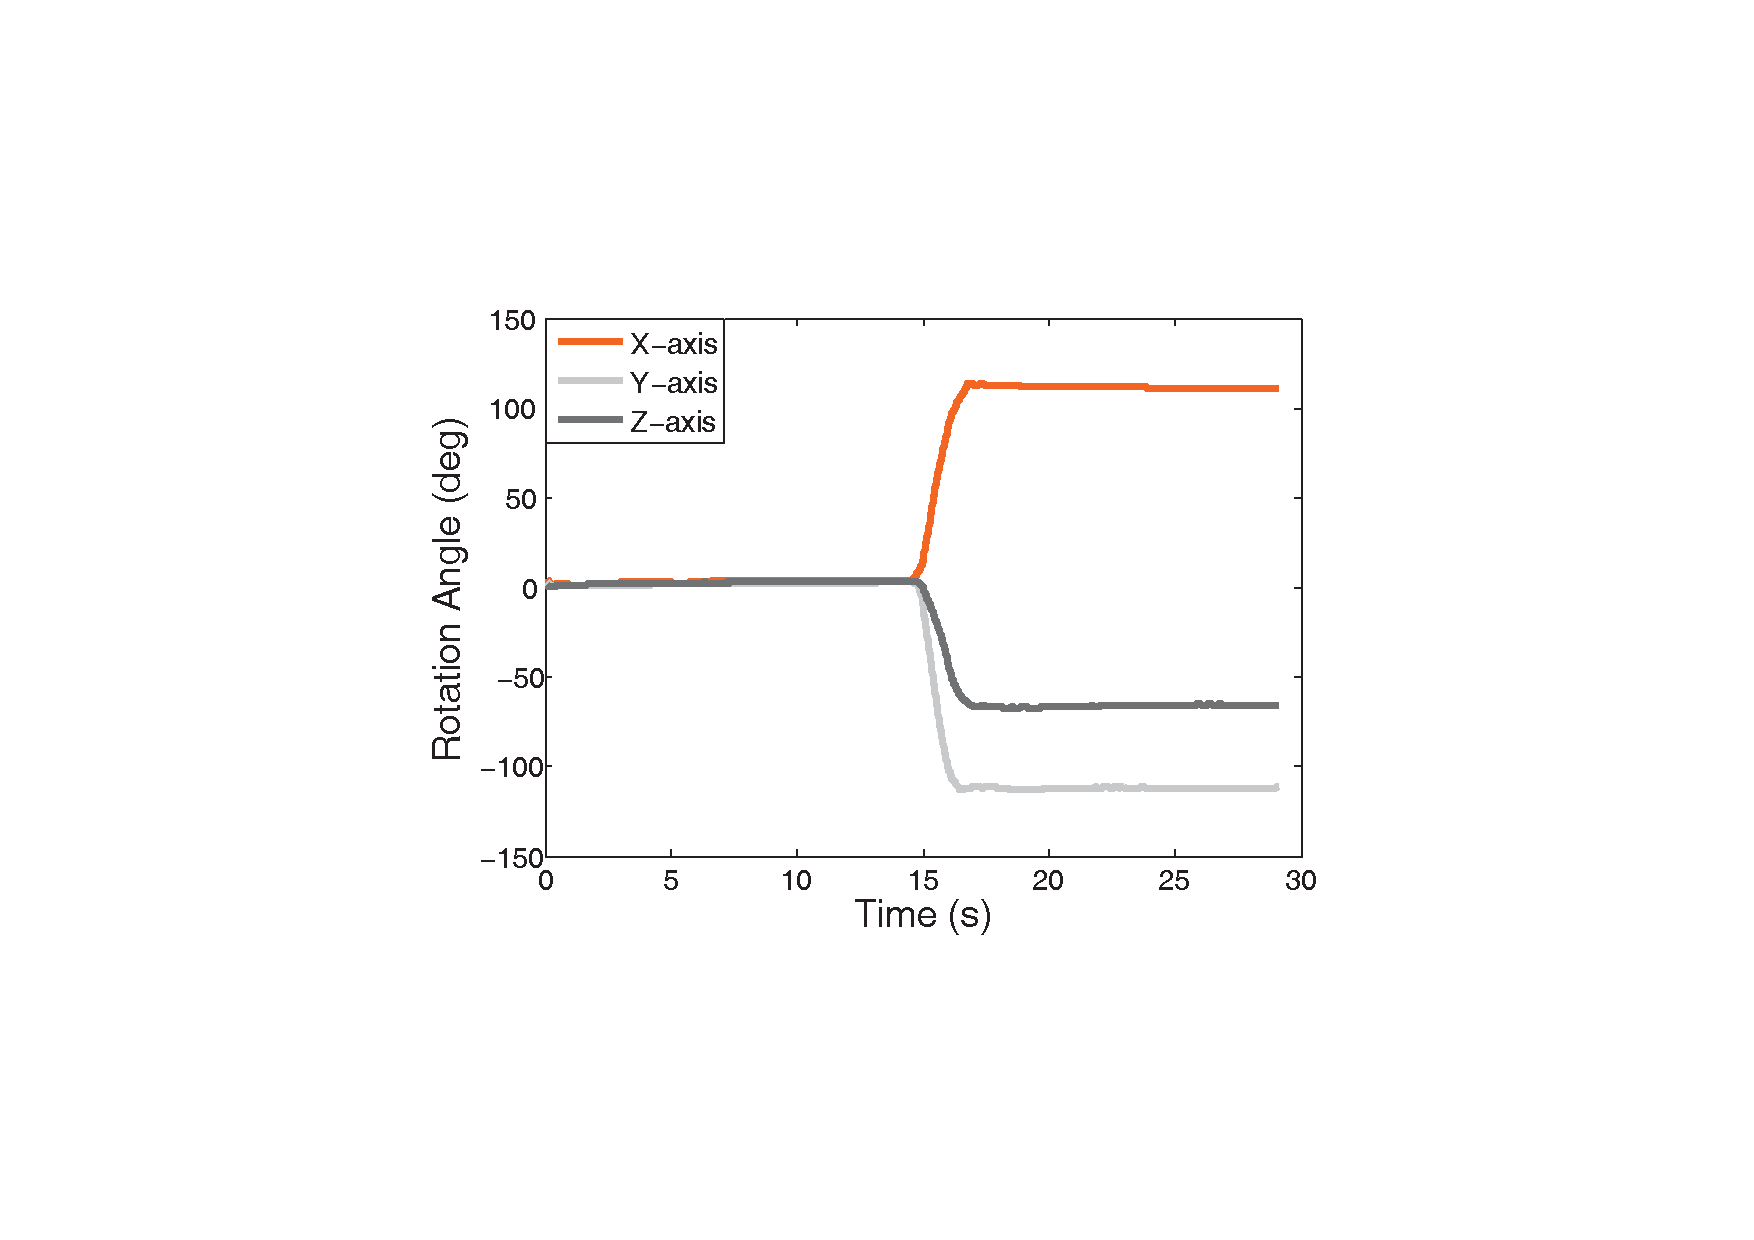
\includegraphics[width=0.32\linewidth]{Figures/BodytoHead.pdf}}
	\subfigure[moving to the abdomen]{\label{BodytoAbdomen}
		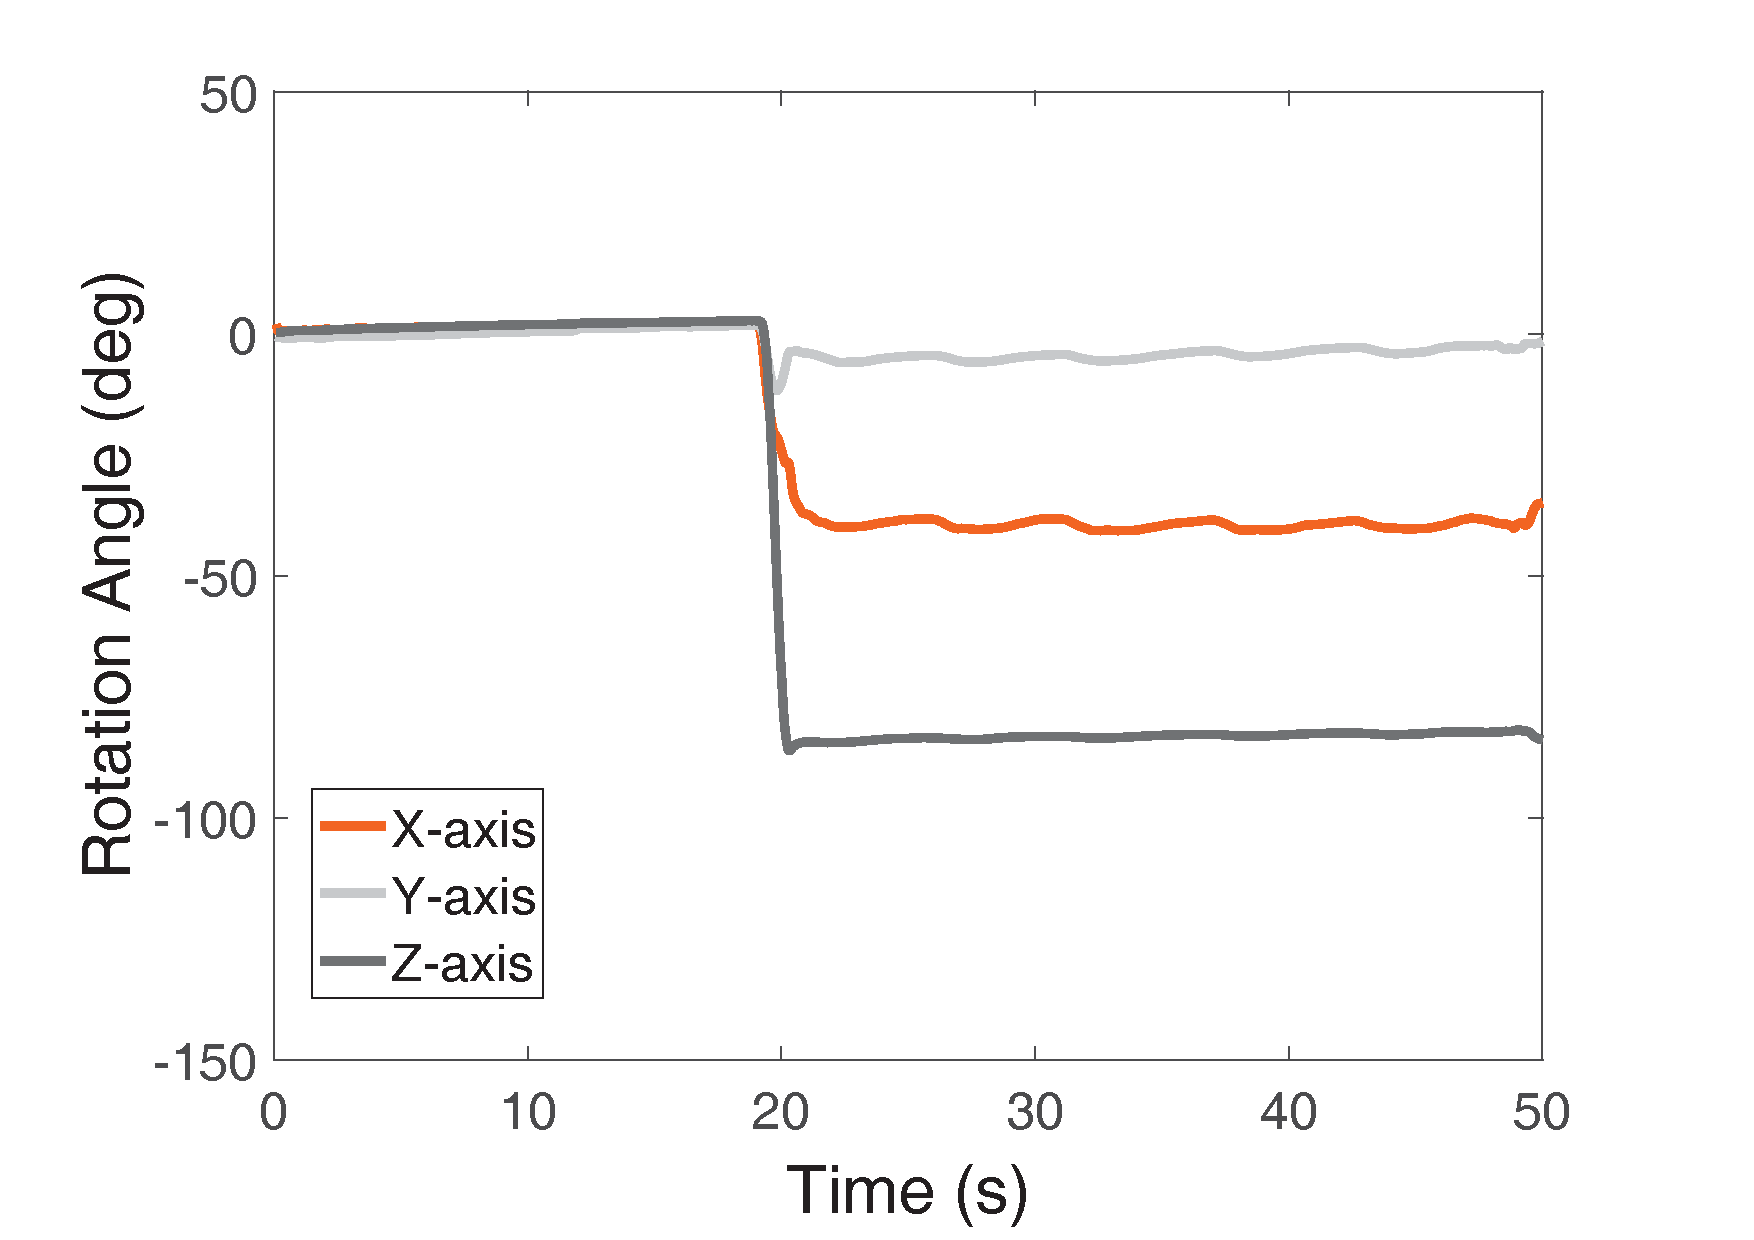
\includegraphics[width=0.32\linewidth]{Figures/BodytoAbdomen.pdf}}
	%  \hfill
	\subfigure[moving to the chest]{\label{BodytoChest}
		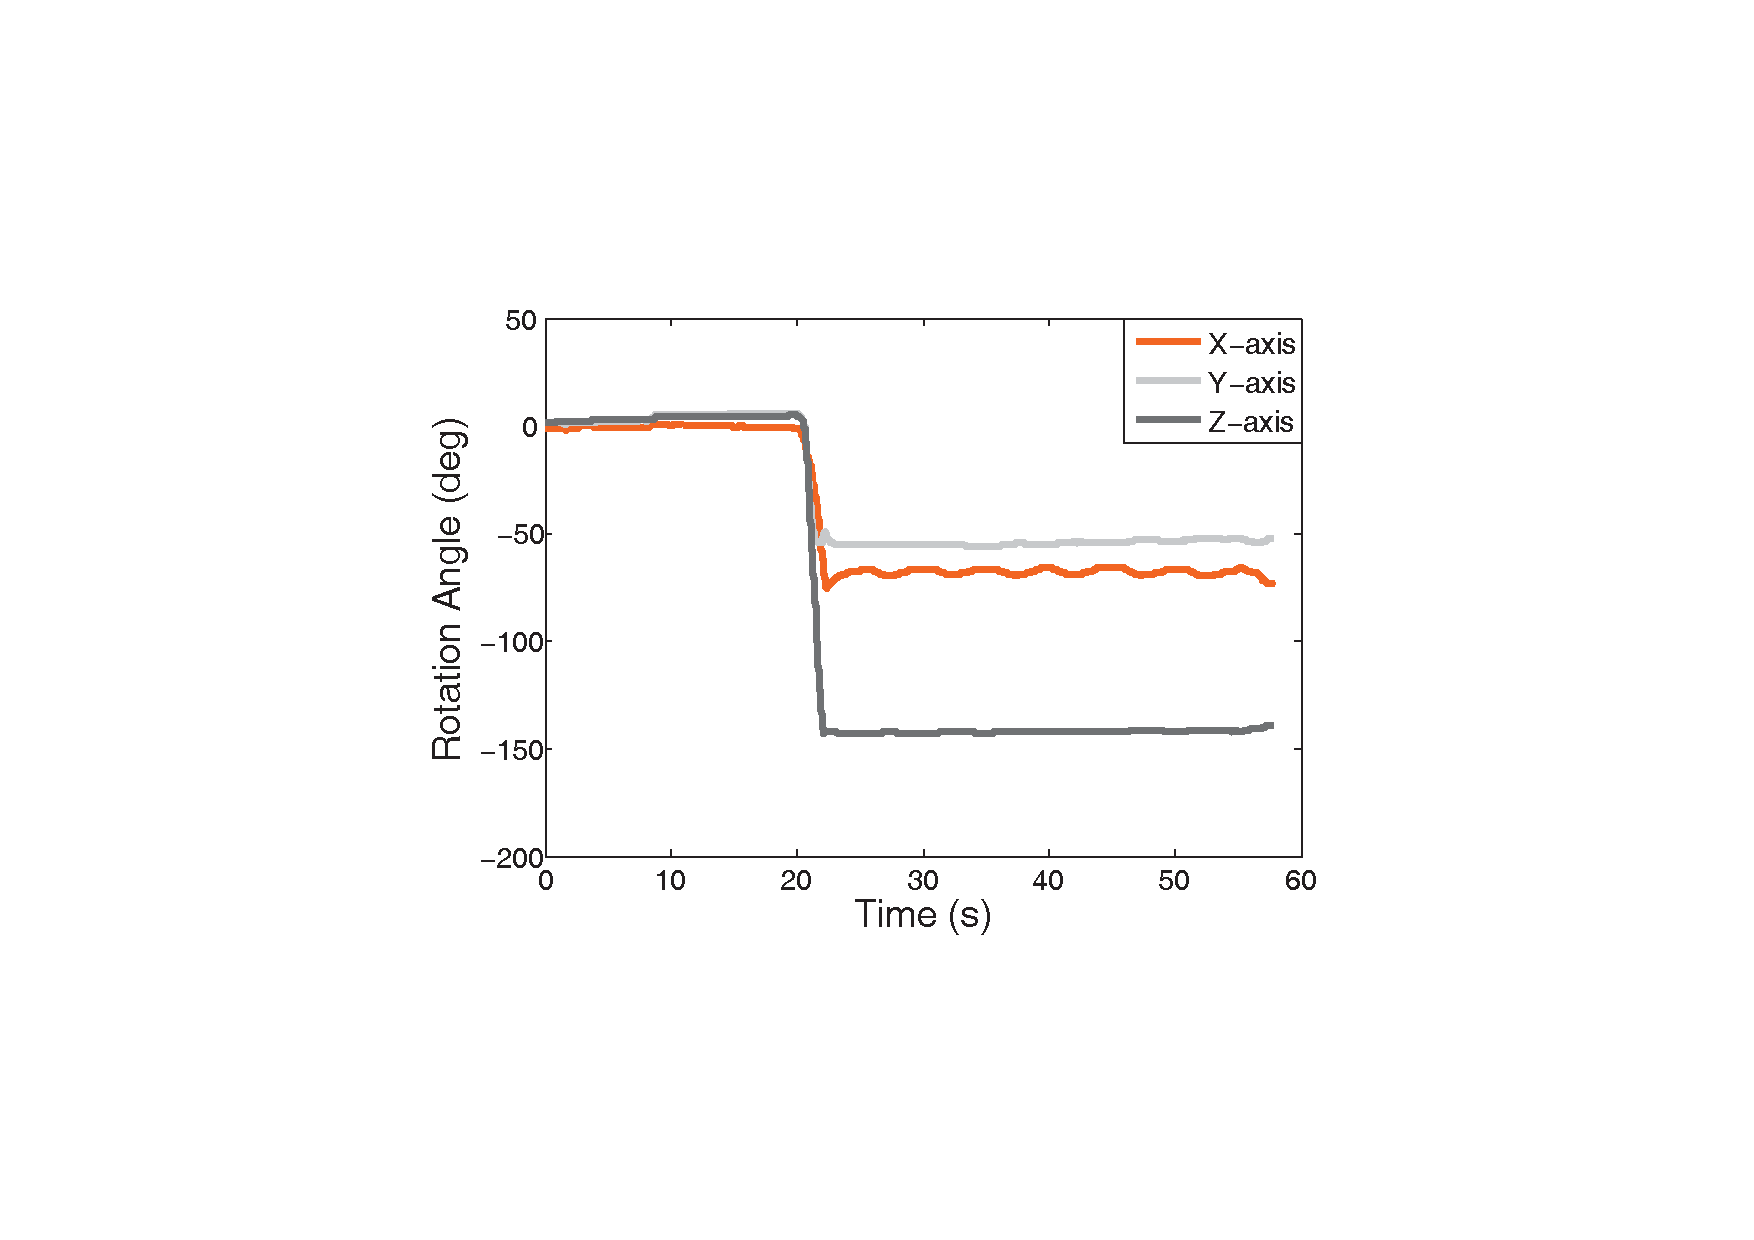
\includegraphics[width=0.32\linewidth]{Figures/BodytoChest.pdf}}
	%  \hfill
  %  \subfigure[moving to the shoulder]{\label{BodytoShoulder}
%		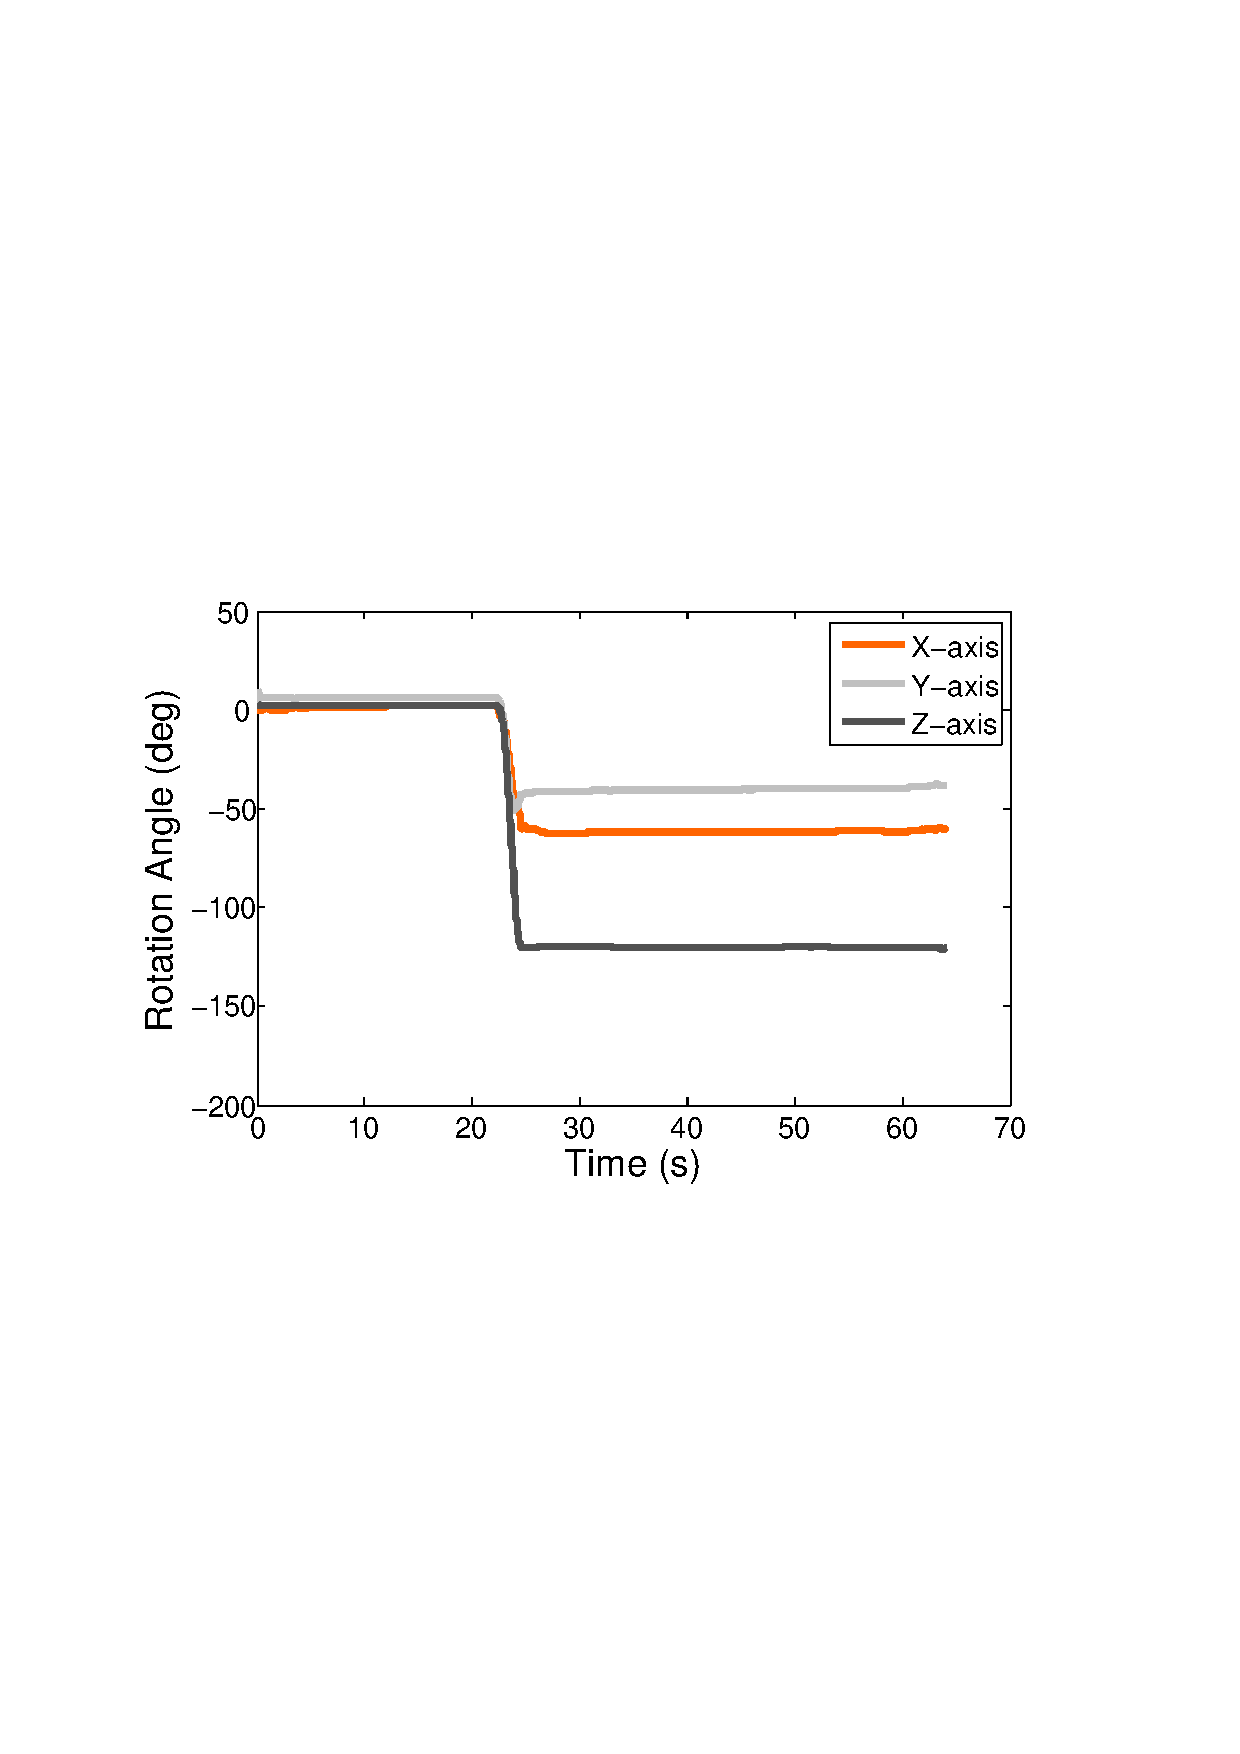
\includegraphics[width=0.34\linewidth]{Figures/BodytoShoulder.pdf}}
	\caption{The differences of the rotation angle when a hand of one of our users, placed next to the subject's body, is moved to his head (a), abdomen (b), and chest (c). }\label{Bodyhand}
\end{figure}

\begin{figure}
	\centering
	\begin{minipage}[t]{.475\textwidth}
	\centering
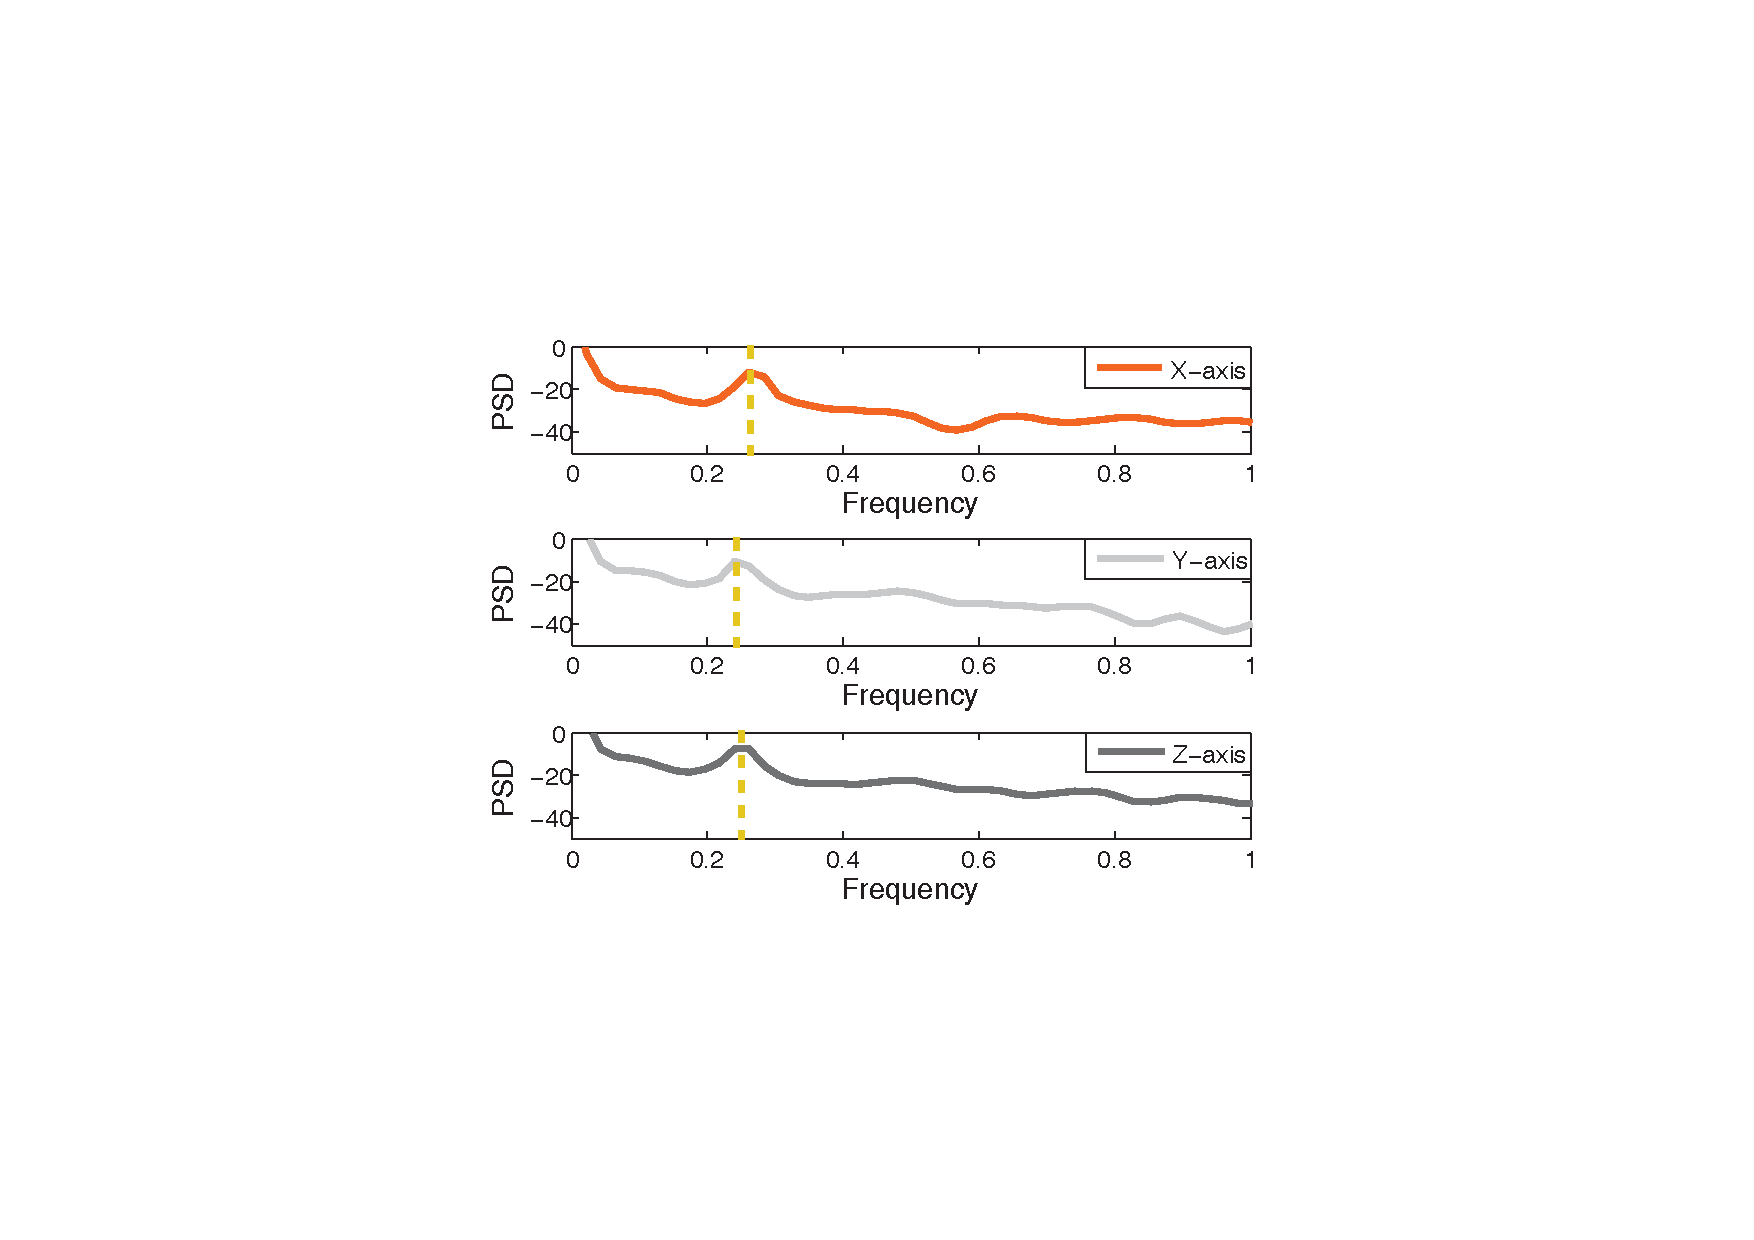
\includegraphics[width=7cm,height=5cm]{Figures/PSD.pdf}
\caption{The power spectral density (PSD) of the accelerometer readings when a user's hand is placed on his chest.}\label{fig:PSD}
	\end{minipage}%
\hfill
	\begin{minipage}[t]{.475\textwidth}
	\centering
	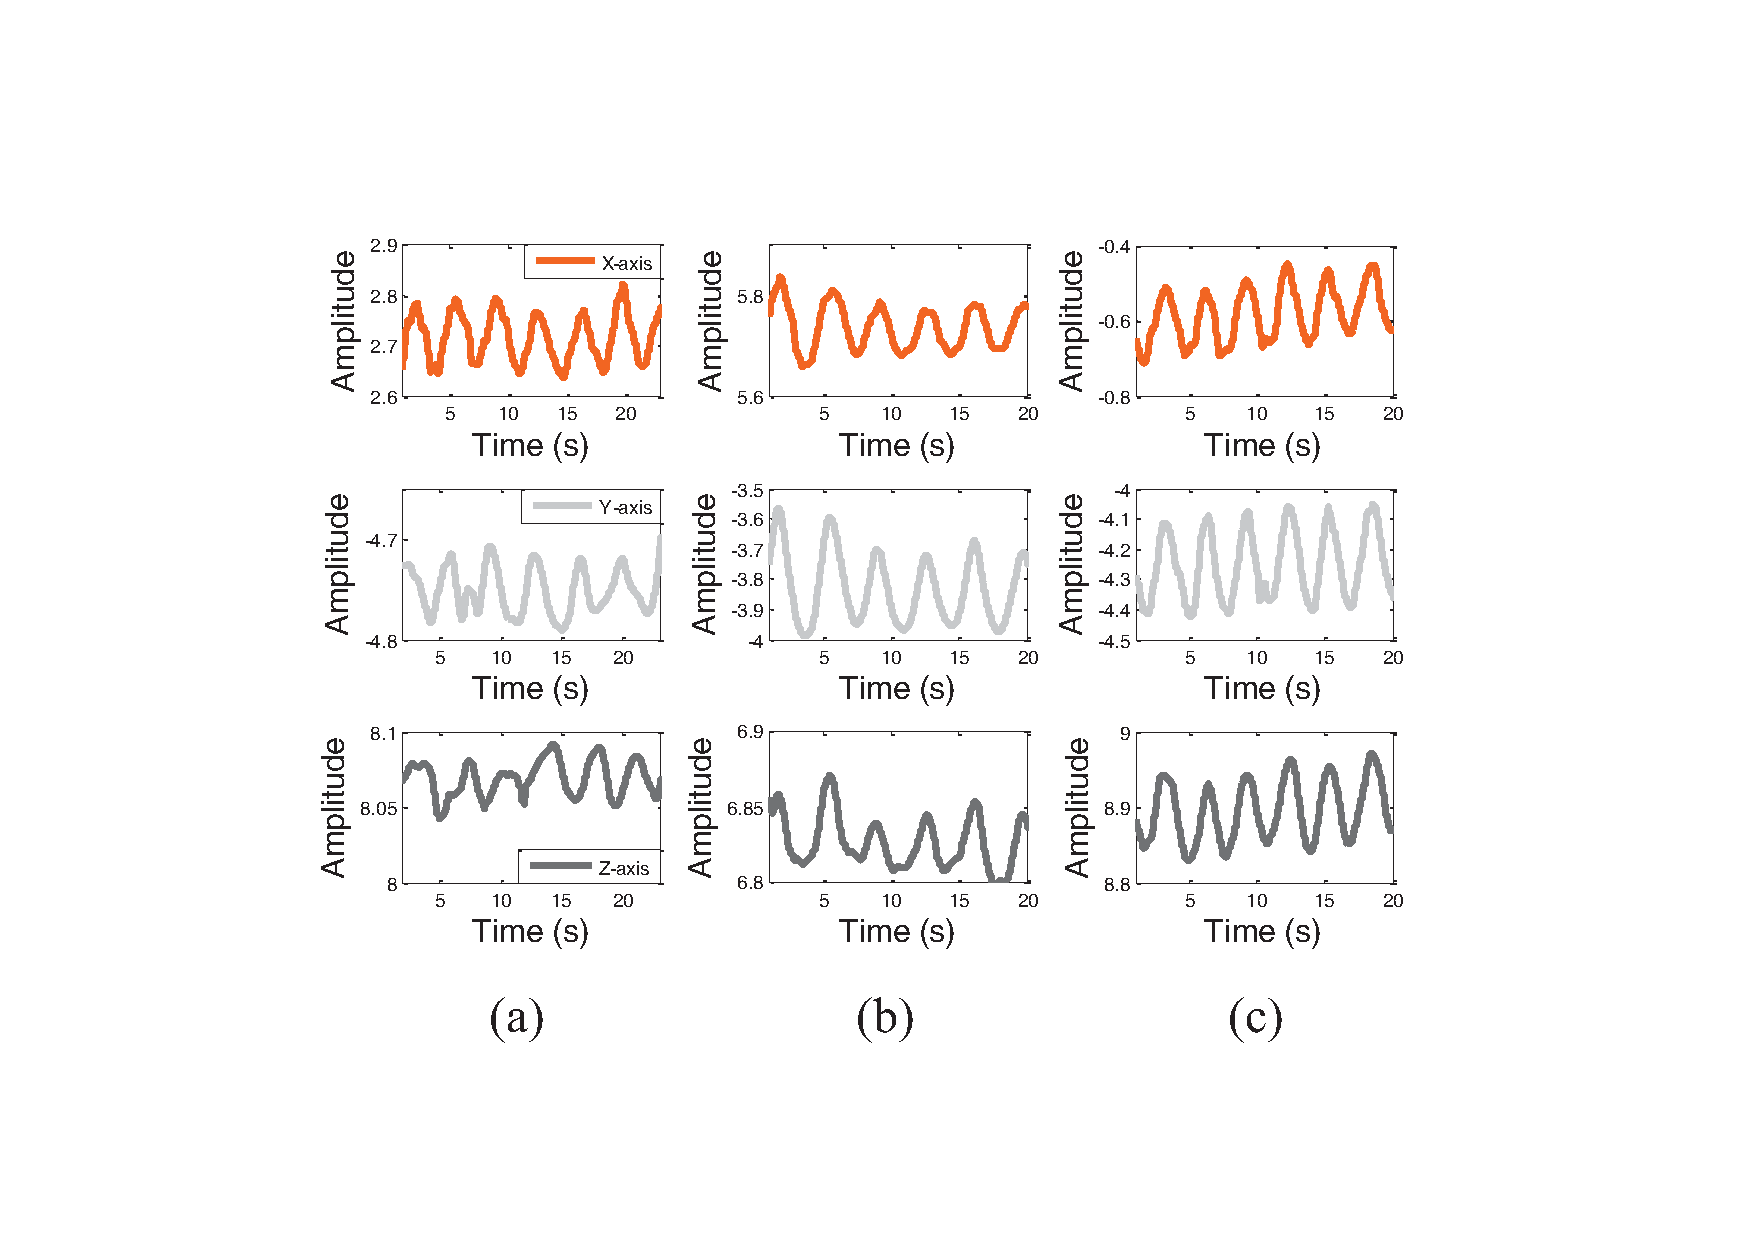
\includegraphics[width=7cm,height=5cm]{Figures/breath_ok1.pdf}
	\caption{The periodic change of the acceleration signal. (a) REM--Location 1. (b) REM--Location 2.  (c) NREM--Location 1.}\label{fig:breath_ok1}
	\end{minipage}
\end{figure}

%result in uniquely identifiable trajectories that are specified by the start and end point of the hand. By comparing information about the latest trajectory against movement templates (analogously to

%that we can identify current hand position by analysing the latest hand trajectory which caused the hand position to change. we have developed a novel algorithm that is based on the key intuition that, before the hand is placed on the body, it experiences a movement from side of the body to the end position, and after that the hand always experiences a movement from one position to the other. Thus we can further integrate the hand movement trajectory to determine the hand position at current time. In {\systemname}, We consider nine kinds of the trajectories of hand, from the side of the body to the abdomen, to the chest, to the head; from the chest to the abdomen, to the head; from the abdomen to the chest, to the head; from the head to the abdomen, to the chest.
%Fig.~\ref{Bodyhand} shows the rotation angle changes in three dimensions (x, y and z), when the hand next to the body is moved to different
%parts of the body. The data are collected using the gyroscope. To aid clarity, we present the data collected from one of the users
%participated in our pilot study, similar behaviors are observed for all other participants. \textcolor{blue}{In the picture, we only show
%the signals from a single subject. This is because after experiments we found that the three hand trajectories of the hand are roughly the
%same in different people. We only show the approximate relative trend to indicate that the difference in the hand trajectory. So we can use
%the three-axis rotation angle calculated by the gyroscope as a feature to establish a sample library, and use the template distance
%matching classifier to identify the final position of the hand. However, if we only use the hand's movement trajectory to determine the
%position of the hand, then we only get the movement relative to a certain known starting position, not the final absolute position of the
%hand. That is, only when we know that each time the starting position of the hand before movement, we can judge the final hand position
%based on different trajectories. However, in practical applications, it is difficult for us to obtain the starting position of the hand
%every time. Therefore, we only cannot rely on the hand movement trajectory to achieve the purpose of detection. However, we found that when
%the hand is placed on the head, the hand placement is clearly different from that of the hand on the chest or abdomen, which makes it
%easier to detect by the angle characteristics calculated by the acceleration when placed on the head. When the hand is on the chest or
%abdomen, the angle characteristics are very similar and difficult to distinguish. Hence, we need an additional verification step to ensure
%the hand is on the chest or abdomen. We can based on key intuition is that we can observe acceleration signals to exhibit a distinctly
%periodic fluctuation, as shown in Fig. \ref{Bodyhand}. This is due to the movement of the abdomen and chest caused by breathing. Therefore,
%we can use the occurrence of respiratory events to determine if the hand is indeed on the body (abdomen or chest). Through the detection of
%respiratory events, we can not only determine the initial position of the hand before movement but also filter out some areas near the
%chest or abdomen, such as the shoulders or hips. This is because when the hand move to the shoulder or hip and some other areas close to
%the chest or abdomen, the resulting hand trajectories are very similar, but we can not observe significant respiratory events, as shown in
%Fig. \ref{BodytoChest} and Fig. \ref{BodytoShoulder}. So we can combine with the hand's movement trajectory to accurately determine the
%hand position.}

\paragraph{Detect abdomen and chest positions.}

\nt{When the hierarchical model predicts the hand to placed elsewhere than the head, it can be located at anywhere, including different
parts of the body. However, in our case we are only interested in detection if the hand is on the chest or abdomen -- or at neither of these positions. We build on the intuition that the hand is likely to be affected by breathing whenever it is placed on chest or abdomen.} Specifically, the
 impact of breathing results in periodical fluctuations on the accelerometer readings. This is because the hand will be pushed up and drop down due to
breathing. \nt{Our experimental data suggest that this behaviour only takes place when 
the hand is placed on the abdomen or the chest, not when the hand is located elsewhere (such as the shoulder). Thus we can separate these two locations from other locations by examining whether the accelerometer values are impacted by respiration.} 

To examine if the accelerometer data are affected by the respiration, we calculate
the power spectral density (PSD) of the collected accelerometer data. \nt{We then check the PSD to see if we can observe any peak that closely matches human
respiratory frequency}. A match indicates that the hand is affected by a respiratory event and hence the hand is likely to be placed on
either the abdomen or the chest. Fig. \ref{fig:PSD} provides an empirical evidence to support our design choice. It shows the PSD for one
of pilot study user when his hand was placed on the chest. Here we calculate the PSD for the accelerometer data collected from the x, y and z directions. We can see from the diagram that there is a large peak located at around 0.25Hz (highlighted in the diagrams) when a
respiratory event is detected (which was verified by video feed). This peak corresponds to the average respiratory frequency of an
adult (0.2Hz to 0.47Hz)~\cite{Breath_frequence}, suggesting that the PSD reading can be used as a proxy to detect respiratory events.
\systemname thus exploits the PSD to detect if the hand is placed on the abdomen or the chest by checking if there is any peak value of PSD
falls within the range of 0.2Hz (corresponding to 12 breathes per minute) and 0.47Hz (corresponding to 28 breathes per minute).

\nt{Putting things together, we thus first use the PSD detector to identify whether a respiratory event is taking place. When respiratory events are detected, we }then use again a kNN
classifier to make a binary decision to determine if the hand is placed on the abdomen or the chest based on the rotation angle readings
(see Fig.~\ref{Bodyhand} b and c). \nt{On the other hand, if no respiratory peak is detected, we assume the hand to be located at another place on the body that is not supported. } Similarly to the head position model, the training samples for the kNN model are also collected from our pilot
study users -- where each training example includes the rotation angle readings when the hand is either placed on the abdomen or the chest.

\subsubsection{Labeling REM/non-REM Stages}

We have also found that the extent of body movements can be used to judge the amplitude of respiration, which in turns allows us to detect
rapid-eye-movement (REM) and non-rapid-eye-movement (NREM) stages. This is based on a prior study showing that when people sleep in the
REM stage, their respiratory amplitude is smaller than that in the other stages~\cite{respiratory1982}. Hence, we can roughly determine the
user's current sleep stage based on the respiratory amplitude. Respiratory amplitude is only an indicator of the division of the sleep
stage and we can not regard it as a basis for final judgement. \nt{However, it serves as an early reference that helps later phases of the sleep
stage detection. Normally chest movement amplitude is smaller than abdominal movement amplitude. However, in
during different sleep stages, respiration amplitudes differ~\cite{respiratory}. Hence, it is likely that there is a situation where chest
movement amplitude in the NREM stages is close to the abdominal movement amplitude in the REM sleep stage. As a result, a na{\"i}ve solution of applying a threshold cannot work satisfactorily but we need to combine it with the position of hand detected earlier. Through 
above steps, we have been able to determine whether the hands are on the chest or abdomen, and then we can go further to determine the
extent of breathing according to the degree of up and down motions, from which we can approximately infer current sleep stage}. Now we take the case of hands
on the abdomen as an example.


Even when the hand is placed on the abdomen, due to minor changes in the exact location of the user's hand, the intensity of
accelerometer fluctuations caused by respiration varies. Hence, we cannot use the amplitude information to determine true respiratory
amplitude directly. This problem is illustrated in Fig.~\ref{fig:breath_ok1}, where (a) and (b) contain triaxial acceleration measurements
at different locations of the abdomen during REM sleep stage, and in (c) which consists of acceleration data for NREM stages at the same
approximate position as in (a). \nt{We can see that when the hand is on the abdomen, but the location differs, we cannot directly judge the respiratory amplitude from the amplitude of the three accelerometer axes.}

\begin{figure}[!t]
\centering
      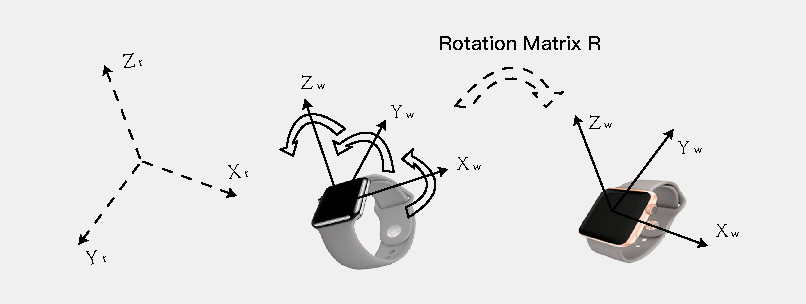
\includegraphics[width=0.67\linewidth]{Figures/watch.pdf}
  \caption{The first figure on the left is the torso coordinate system, and $Y_t$ points north. The middle figure shows the watch coordinate system when the watch an arbitrary position, and the right of the figure shows that the  watch coordinate system after we completed the coordinate system conversion.}\label{fig:watch}
\end{figure}

To solve this problem, we convert the acceleration data from the wristwatch coordinate system into the torso coordinate system. \nt{As breathing results in chest moving up and down, movements along the z-axis in the torso coordinate system can be used to identify respiratory amplitude}. We express the tri-axial acceleration data as $Acc_w$ = [$X_w$, $Y_w$, $Z_w$] in the wristwatch coordinate system and $Acc_t$ = [$X_t$, $Y_t$, $Z_t$] in the torso coordinate system, as shown in Fig.~\ref{fig:watch}. \nt{Our coordinate alignment aims to find a rotation matrix $R$ that aligns the watch's coordinate system with the torso coordinate system ({[$X_t$, $Y_t$, $Z_t$]}). Matrix $R$ can be obtained from the three-axis direction information of the orientation sensor. Specifically, we have:} %After the coordinate system is aligned, the angle between the y-axis of the wristwatch coordinate system and the y-axis of the torso coordinate system is 180 degrees.
\begin{equation}
      X_t  = (X_w {\cos\gamma} + Y_w{\sin\gamma}){\cos\theta} + (Y_w\cos\sigma + Y_w\sin\sigma)\sin\theta,
\end{equation}
\begin{equation}
      Y_t = -((Y_w\cos\sigma + Y_w\sin\sigma)\cos\theta - (X_w\cos\gamma + Y_w\sin\gamma)\sin\theta),
\end{equation}
\begin{equation}
      Z_t = (Z_w\cos\gamma - Z_w\sin\gamma)\cos\sigma - (Z_w\cos\gamma - Z_w\sin\gamma)\sin\sigma,
\end{equation}
where $\theta$, $\sigma$ and $\gamma$ are the x, y and z axis data of the orientation sensor respectively, representing the direction angle, the tilt angle and the roll angle collected from the orientation sensor. After alignment, we can see in Fig.~\ref{fig:cordi} that the z-axis shows a periodic signal with significant fluctuations, \nt{while the x- and y-axis data undergo smaller changes around zero, which is consistent with stable sleep influenced only by respiratory patterns.} %the actual situation that when the person is in the supine posture with the abdomen up and down caused by respiration.

 \begin{figure}[!t]
\centering
      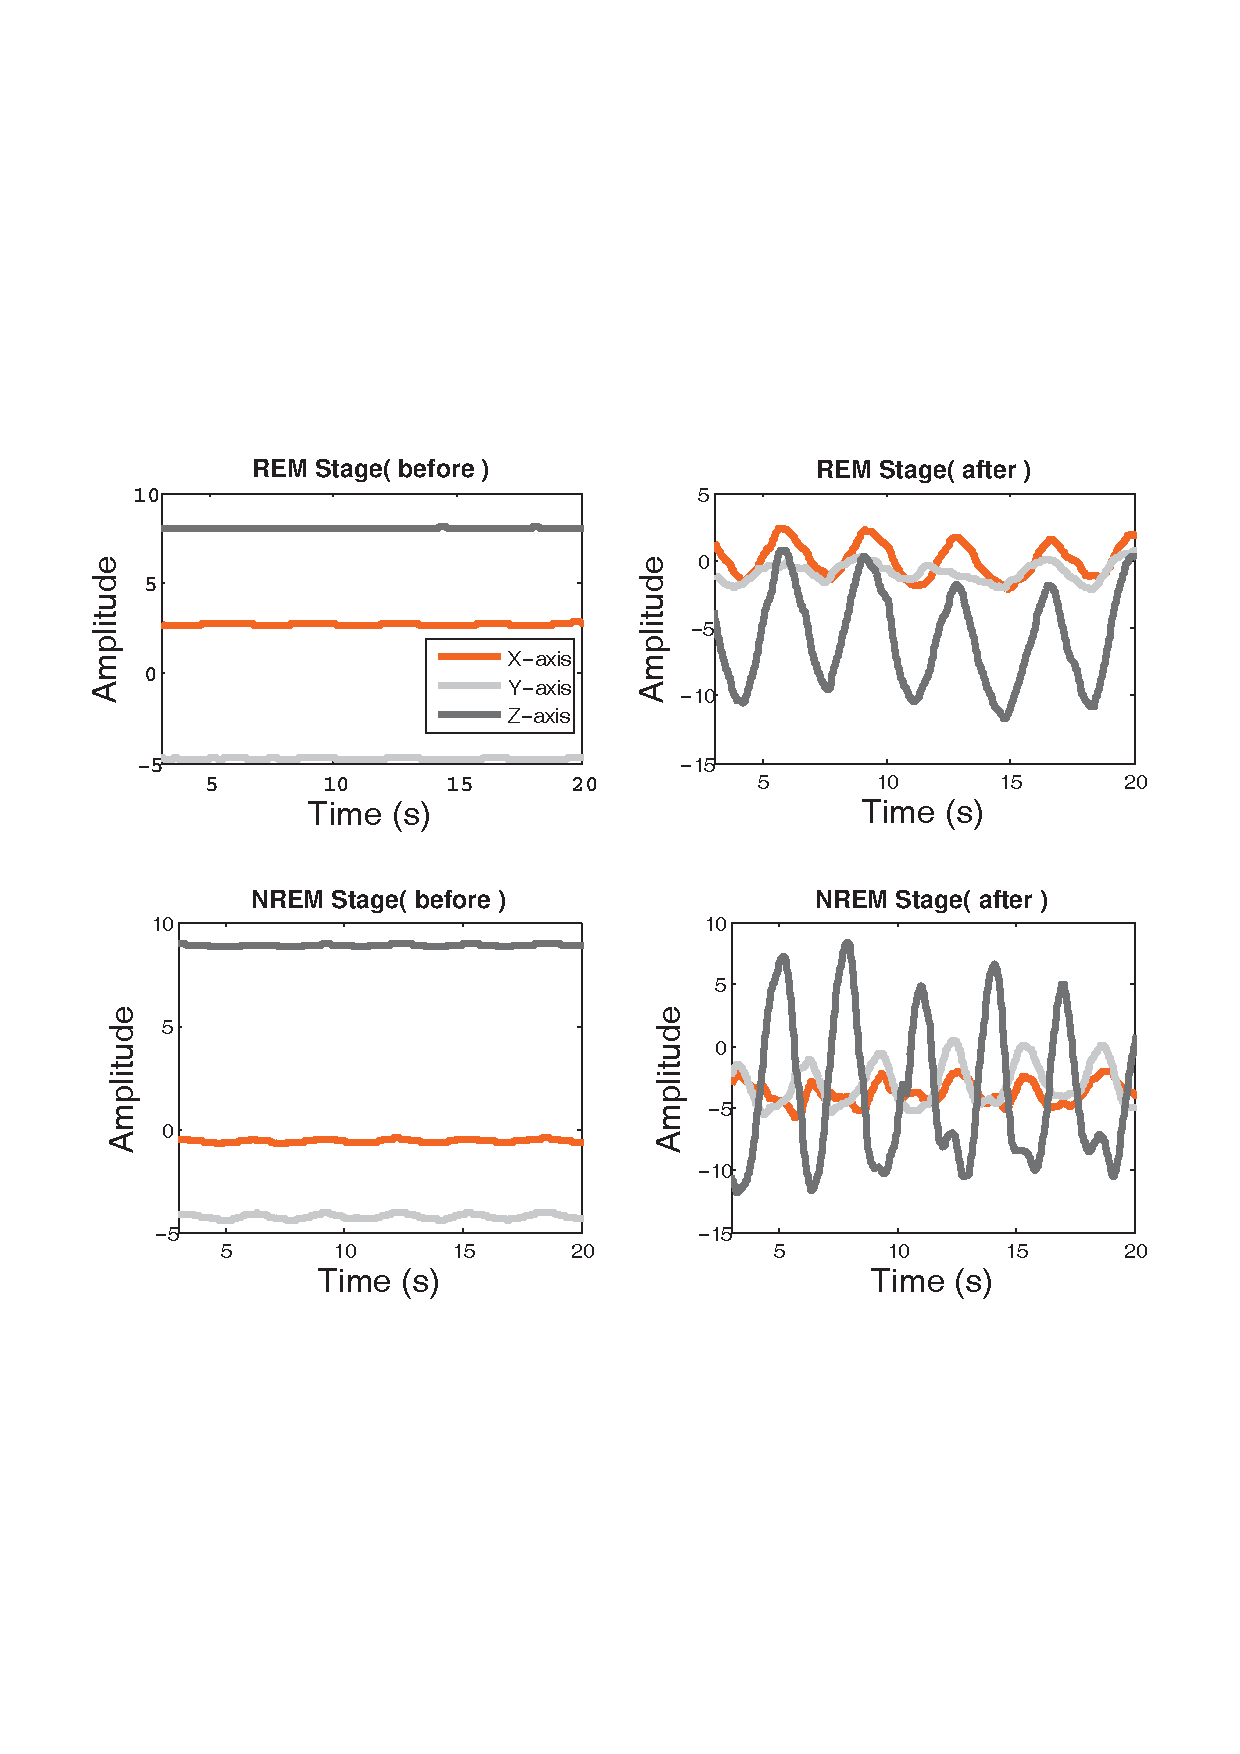
\includegraphics[width=0.75\linewidth]{Figures/cordi.pdf}
  \caption{Acceleration data for different sleep stages.}\label{fig:cordi}
\end{figure}

The two graphs on the left of Fig.~\ref{fig:cordi} show the same acceleration data as has been used in (a) and (c) of
Fig.~\ref{fig:breath_ok1}, respectively. The two right-most graphs correspond to data after coordinate system alignment.  We
can see that, prior to alignment, we cannot effectively distinguish the respiratory amplitude of REM and NREM stages from the
acceleration amplitude. After coordinate alignment, the respiratory amplitudes are clearly visible from the z-axis data. \nt{To separate REM and NREM stages,} we calculate
the variance of z-axis acceleration and use it as a feature to measure the intensity of the fluctuation in a signal, with larger variance
corresponding to greater breath amplitude. Note that we cannot use the sum or magnitude of the z-axis as a measure of intensity as the
measurements remain affected by gravity.

To summarize, we use respiratory amplitude to detect when the user is in the REM stage. We calculate respiratory amplitude when the hand is found to be placed on the abdomen or the chest. \nt{Note that as \systemname operates using a wrist worn device, it can only detect respiratory events when the hand is placed one of these two position. As measure of respiratory amplitude, we use }the variance of z-axis acceleration. We then use a kNN classifier to find from our training examples, which training example is most similar to the input respiratory amplitudes collected from z directions. The similarity is measured by calculating the distance on the feature space. We then use the label (either REM or NREM) associated with the nearest training
example as the classification outcome.

%To generate the training examples, we first use our hand position recognition algorithm described in
%Section~\ref{sec:handpr} to detect, from our training dataset (see (Section~\ref{sec:trainingdata}), whether the hand was placed on the
%abdomen or the chest to calculate the respiratory amplitude. We can consider the user is at either (1) the NREM stage if a large repository
%amplitude (i.e., the amplitude value is not less than 15) is detected, or (2) the REM stage if a normal repository amplitude (i.e., the
%amplitude value is not greater than 4) is detected. These thresholds are chosen based on prior study\FIXME{ \cite{}}. To remove the noises
%of the training data, we only use training examples where both our approach and Fitbit reach the consensus on the eye movement stage. We
%also manually inspect the recorded videos to label the stage from our training data.



%\textcolor{blue}{We then trained a classifier based k-nearest neighbor model (with k = 1) using this feature when the hand is placed on the
%abdomen and on the chest under both REM stage and NREM stages to determine a mapping from current respiratory amplitude to placement. Here,
%we define the respiratory amplitude in the NREM stage as large respiratory amplitude, and the respiratory amplitude in the REM stage as
%normal respiratory amplitude. As for the acquisition of sleep stage, we confirm the label of it when both Fitbit and {\systemname} reach a
%consensus. At the same time, We also take into account video recorded by the camera to manually label part of the respiratory. The
%combination of these three kinds of equipment can enable us to obtain real and accurate data as much as possible.  As classifier we used a
%decision stump which was trained on 200 sets of acceleration data (100 sets of these from the larger respiratory amplitude and the rest of
%sets from the normal respiratory amplitude ) from 10 volunteers, who are randomly recruited by us aged 16 to 60 years old.  The resulting
%threshold for the acceleration variance is around 15 when the hand on the abdomen, and around 4 when the hand is placed on the chest.}
%


\subsection{Body rollover counts \label{sec:bodyrollover}}

Under normal circumstances, people usually rollover their body around 20-45 times a night. The main function of body rollovers is simply to
maintain a comfortable sleeping position as maintaining the same position for prolonged period will result in muscular tension due to
hindered blood supply, which can also lead to local numbness~\cite{rollover2014}. So body rollover is another key indicator about the sleep
quality. {\systemname} can detect the number of body rollovers, which can get some reflections of sleep status and the roll-over frequency
can also help us to classify the sleep stage~\cite{rollover2007}. In general, there are six cases: four posture transition cases between
the supine posture and lateral (left or right) posture, and two posture transitions between the left lateral posture and right lateral
posture. Fig. \ref{fig:BodyRollover} shows the case when the body moves from the left side to the right side.
%
The most intuitive way for detecting body rollover events is to estimate the rotation direction of the arm based on the
rotation angle given by the gyroscope. However, doing so is non-trivial because different users can exhibit drastically different patterns
for arm rotations; and the subtle changes in the starting arm position for the same sleeping posture could lead to a misprediction. As an
alternative to the rotation angle, we find that the tilt angles to be useful for this task because they strongly correlate to a body
rollover event. This correlation thus enables us to effectively translate the change of the tilt angle to a body rollover event to count
the occurrence of such events. Specifically, the angle values of three different axes are on the falling edge or rising edge
simultaneously during a very short time period. Fig. \ref{fig:LeftToRight} -- Fig. \ref{fig:RightToLeft} shows the value changes under
different body rollover cases. To this end, a naive method to detect rollovers would be to rely on changes in angle measurements. However,
this method suffers a very large error since other hand movements will also induce a similar change.

\begin{figure*}[!t]
%\centering
%   \setlength{\abovecaptionskip}{-2pt}
% \setlength{\belowcaptionskip}{-9pt}
\begin{minipage}[t]{0.31\linewidth}\centering
    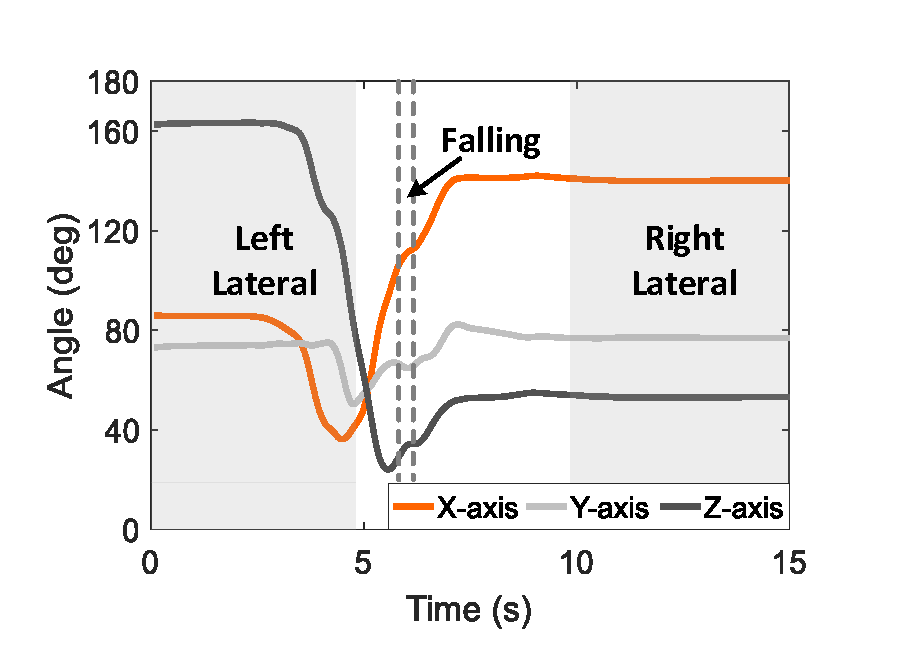
\includegraphics[width=0.97\linewidth]{Figures/LeftToRight.pdf}\centering
  \caption{From left lateral posture to right lateral posture.}\label{fig:LeftToRight}
\end{minipage}
\hspace{2pt}
\begin{minipage}[t]{0.31\linewidth}\centering
    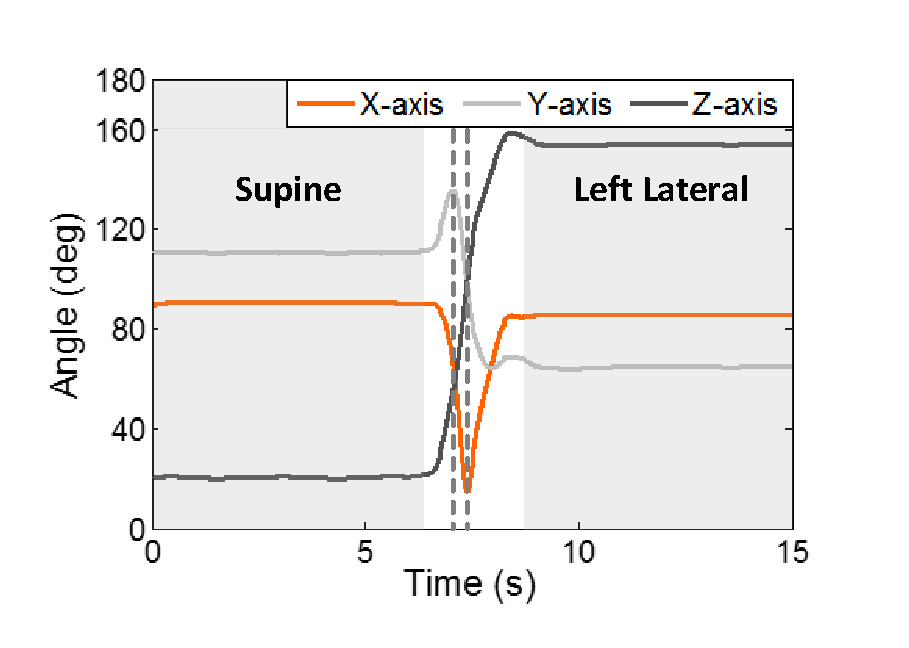
\includegraphics[width=0.97\linewidth]{Figures/SupineToLeft.pdf}\centering
  \caption{From supine posture to left lateral posture.}\label{fig:SupineToLeft}
\end{minipage}
\hspace{2pt}
\begin{minipage}[t]{0.31\linewidth}\centering
    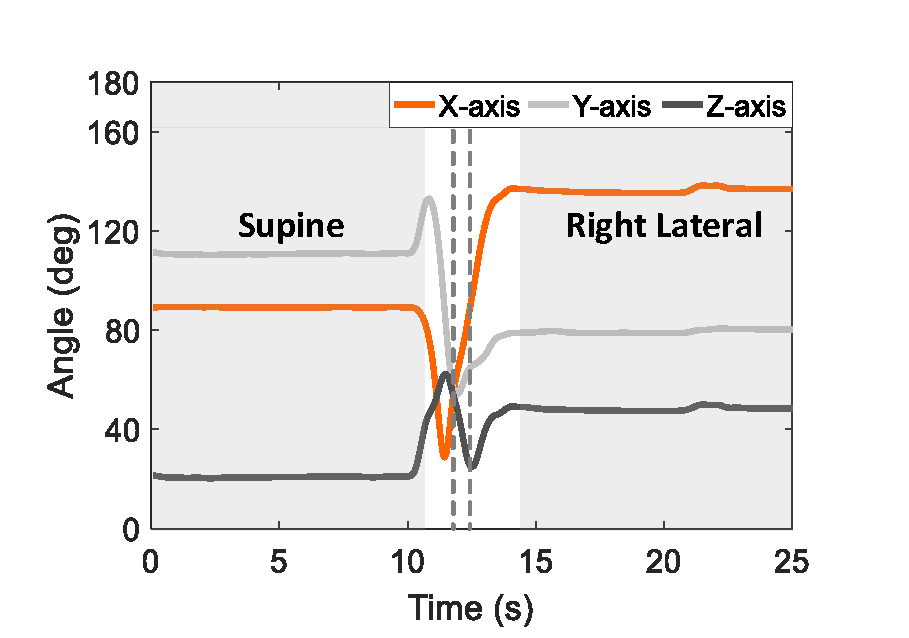
\includegraphics[width=0.97\linewidth]{Figures/SupineToRight.pdf}
  \caption{From supine posture to right lateral posture.}\label{fig:SupineToRight}
\end{minipage}
\end{figure*}

\begin{figure*}[!t]
\begin{minipage}[t]{0.31\linewidth}\centering
    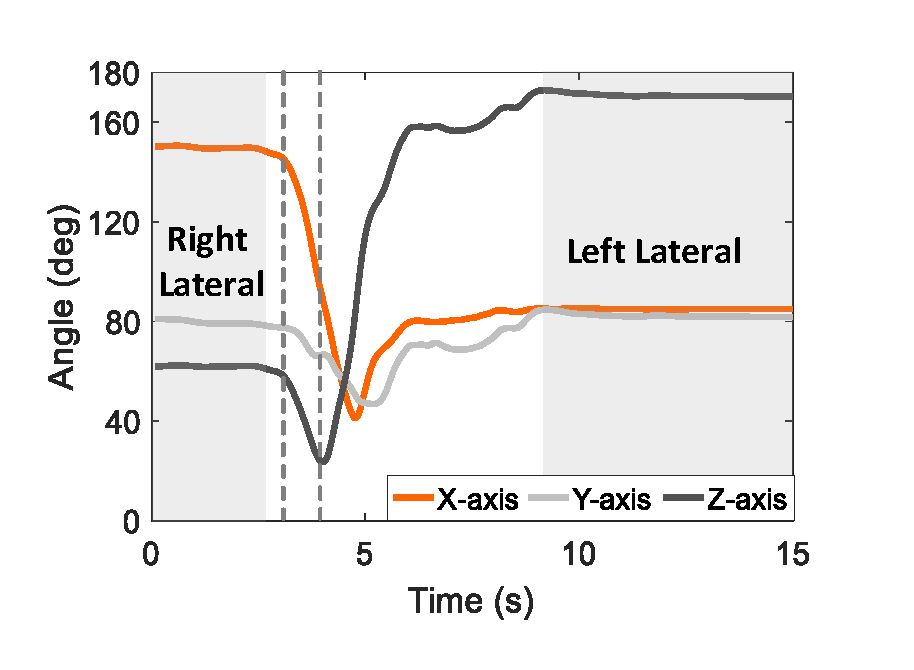
\includegraphics[width=0.97\linewidth]{Figures/RightToLeft.pdf}
  \caption{From right lateral posture to left lateral posture.}\label{fig:RightToLeft}
\end{minipage}
\hspace{2pt}
\begin{minipage}[t]{0.31\linewidth}\centering
    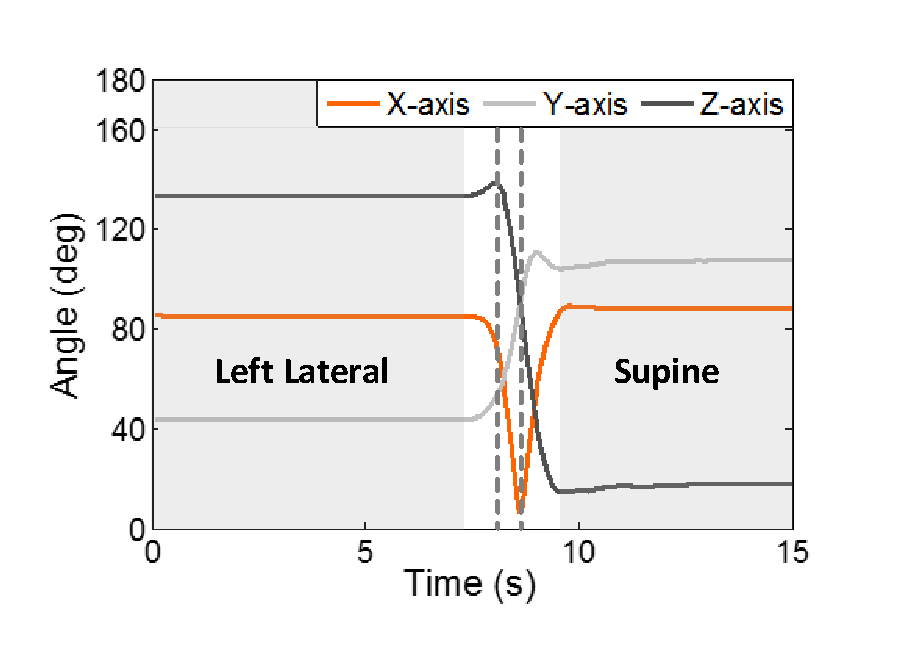
\includegraphics[width=0.97\linewidth]{Figures/LeftToSupine.pdf}
  \caption{From  left lateral posture to supine posture.}\label{fig:LeftToSupine}
\end{minipage}
\hspace{2pt}
\begin{minipage}[t]{0.31\linewidth}\centering
    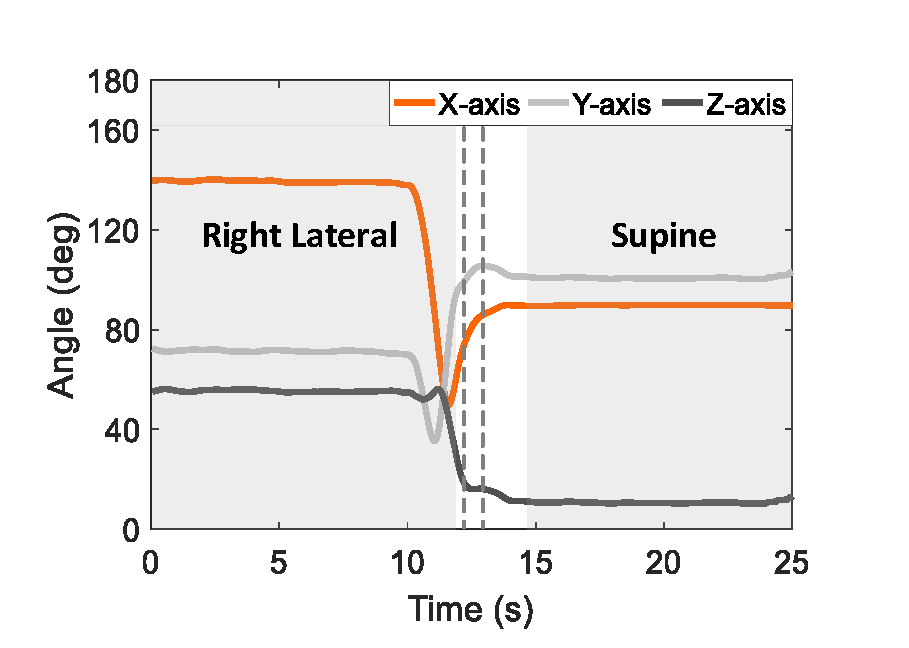
\includegraphics[width=0.97\linewidth]{Figures/RightToSupine.pdf}\centering
  \caption{From right lateral posture to supine posture.}\label{fig:RightToLeft}
\end{minipage}
\end{figure*}

To deal with this challenge, we incorporate the body postures to improve the detection accuracy. As shown in Fig. \ref{fig:BodyRollover},
the body postures are different before and after the rollover. Therefore, after we detect the time when the angle values changes, we term
the time as a possible rollover time point. Then we use the sleep posture classification algorithm to determine whether the body postures
are the same or not over a period of time before and after this point. If the postures are the same, we exclude this time
point, otherwise a body rollover event is found. In other words, a body rollover event is recorded when the posture changes are detected
between two time points. Note that {\systemname} not only counts the number of rollovers, but also reports the exact nature of the
rollover event.


\subsection{Detecting micro-body movements \label{sec:microbo}}

Besides major body movement, such as rollovers, there often are involuntary body movements that can affect sleep quality. With the deepening of sleep, limbs are extremely relaxed, and a little stimulus will produce trembling and micro beating. Such behavior is most likely to occur during the deep sleep stage and the REM stage~\cite{ancoli2003role,Jean2000Sleep}. Therefore, by detecting such micro body movements and distinguish them from large body movements can help us to further analyze the user's sleep stage. In this paper, we are interested in the sleep-related body movements including hand moving, arm raising, and body trembling.

One of the challenges in detecting the micro-body movements is to cancel the inherent noises brought by the accelerometer.
To cancel the noises, we apply a moving window to the collected accelerometer data points to minimize the impact of the outliers. To
determine the size of the moving window, we apply different parameter settings to our training data. We found that a moving widow with a
size of 35 gives the best average results on our training set. Therefore, we choose to apply a moving window of 35 sample points to the
collected user data and then calculate Root Sum Square (RSS) for the data points within a window:

\begin{equation}
      Rss(t) =\sqrt{(acc_x(t))^{2}+(acc_y(t))^{2}+(acc_z(t))^{2}},
\end{equation}
$acc_x(t)$, $acc_y(t)$ and $acc_z(t)$ represent the accelerometer sample value of x-axis, y-axis and z-axis at time stamp t respectively.


We can obtain the first-order derivative of from the RSS values:
\begin{equation}
      V(t)=Rss(t)-Rss(t-1).
\end{equation}

Eventually, we set the threshold to be 0.03, which can achieve a satisfactory detection performance. We also observe that the micro movement duration is very short, which lasts less than 2 s.
However, in our body rollover experiments, we find that the average movement duration is 3 s, as shown in Fig. \ref{fig:LeftToRight} - Fig. \ref{fig:RightToLeft}.
Therefore, we can first divide the body movement events into large movement and micro movement by detecting the signal duration time.

To distinguish among the micro-body movements of hand movement, arm raising and body trembling, we first consider the
duration of the movement. We observe from our training data that an arm rising action typically takes around 1.8 second, while a hand
movement and a body trembling take around 1 second. Using the duration of the movement, we can distinguish arm rising from the other two
movements. We also find that the body trembling tends to lead to a more drastic change in the accelerometer readings compared to the hand
movement. This observation is depicted in Fig.{fig:micro-move} using samples from one of our training users. Based on this observation, we
then use the change of accelerometer reading to distinguish between the body trembling and the hand movement. We do so by calculating the
first-order derivative of accelerometer data to find out the peak of the acceleration data.  If the peak is great than 1.5 and the duration
of the movement took between 0.8 and 1.2 second, a body trembling is detected; if the peak is less than 1 and the duration of the movement
took between 0.8 and 1.2 second, a hand movement is detected; otherwise, if the duration of the movement took between 1.5 and 2 second, an
arm rising is detected. These thresholds are empirically determined from our training data.

%\textcolor{blue}{In order to distinguish micro-body movements, including hand movement, arm raising and body trembling, it is very
%intuitive to detect based on the duration of the movement, because we find that the durations of these movements are significantly
%different.
%So we try to use the duration of these movements to perform detection. However, we find that the average duration of the arm rising is 1.8 s, but the duration of the other two types of movement is around 1 s,
% so it is difficult to set a suitable threshold to accurately detect them. Therefore, only through the duration of the movement we can only detect the arm rising with obvious feature.
% For the hand movement, and body trembling is not effective. However, we have found that body  trembling is a sudden movement event, which leads to a more pronounced change in acceleration,
% so we can use acceleration changes to distinguish them based on such an observed fact. Specifically,  as we can see from the figure,  acceleration of body trembling has a more pronounced peak when compared to the hand movement.
% So we perform peak detection on the first-order derivative of the acceleration.}
%
% So we perform peak detection on the acceleration variance. For the detected peak, we calculate the difference $d$ between the peak of the accelerometer data and the average peaks of the accelerometer readings in our training data.
%
%\begin{equation}
%      d=\mid(peak-average(oi))\mid,
%\end{equation}
%$oi$ indicates the type of micro-movement, when $oi$ is 1, it indicates the hand movement and 2 represent body trembling.
%

\begin{figure}[!t]
\centering
      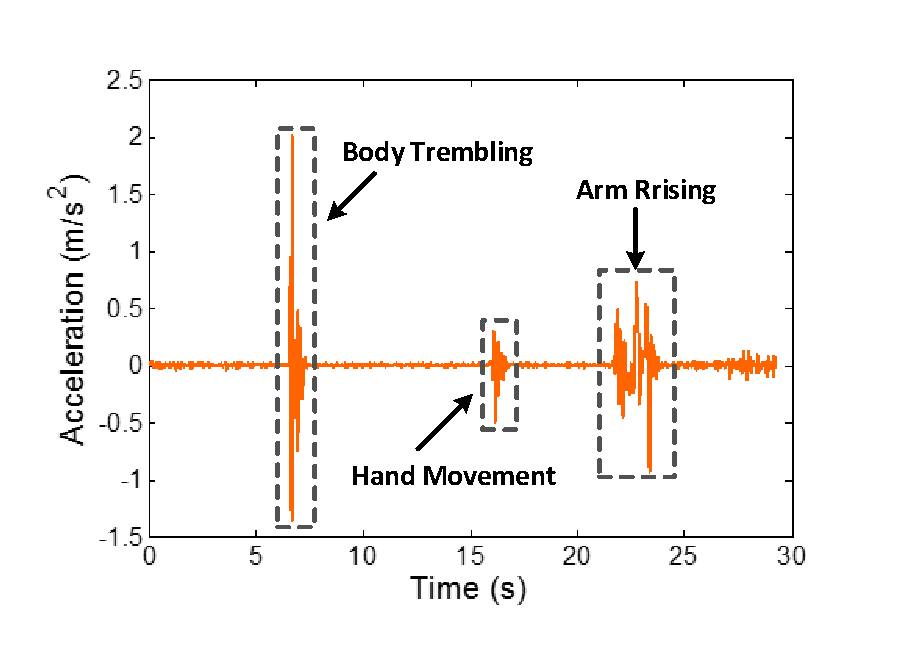
\includegraphics[width=0.43\linewidth]{Figures/Micromovement.pdf}
  \caption{Accelerometer readings for micro body movements using samples from one of our training users.}\label{fig:micro-move}
\end{figure}

%For the two types of potential micro-movements to be classified, we calculate variances for 100 sets of micro-movement data for these 10 volunteers and perform peak detection, as well as make these peaks as features for a particular type of movement to establish a reference data set. In order to classify the micro-movement more accurately, we further obtain the average of the peak features ($average(oi)$) in the reference data set. And then we determine the type of micro-movement with the smallest value of d as the final detection result.


\subsection{ Detecting Acoustic Events \label{sec:acoustic}}
Acoustic events during sleep, such as snore, cough and somniloquy, can reflect and affect user's sleep quality and physical health. For
example, snore is one of the possible symptoms of cerebral infarction patients.  And long-term snoring can also have a serious impact on
health and sleep. It can cause behind sleep apnea or narcolepsy, a sleeping disorder~\cite{snoring2016,snoring2013}. And when there is a
cough, the human cerebral cortex cells are always in an excited state, limiting the depth of sleep, allowing only short sleep between
wakefulness, like many other sleep disruptions. {\systemname} can detect these different acoustic events, including snore, cough and
somniloquy. \ Classical acoustic algorithms use multi-dimensional features to detect acoustic events from a complex
environment~\cite{gu2016sleep}. By contrast, We tailor our design to the problem domain to derive a simpler yet effective acoustic
detection algorithm, by exploiting the characteristics of the different events that we target.

\begin{figure*}[!t]
\centering
%   \setlength{\abovecaptionskip}{-2pt}
% \setlength{\belowcaptionskip}{-9pt}
%\begin{minipage}[t]{0.32\linewidth}\centering
 \subfigure[Snore of six times.]{\label{snore}
   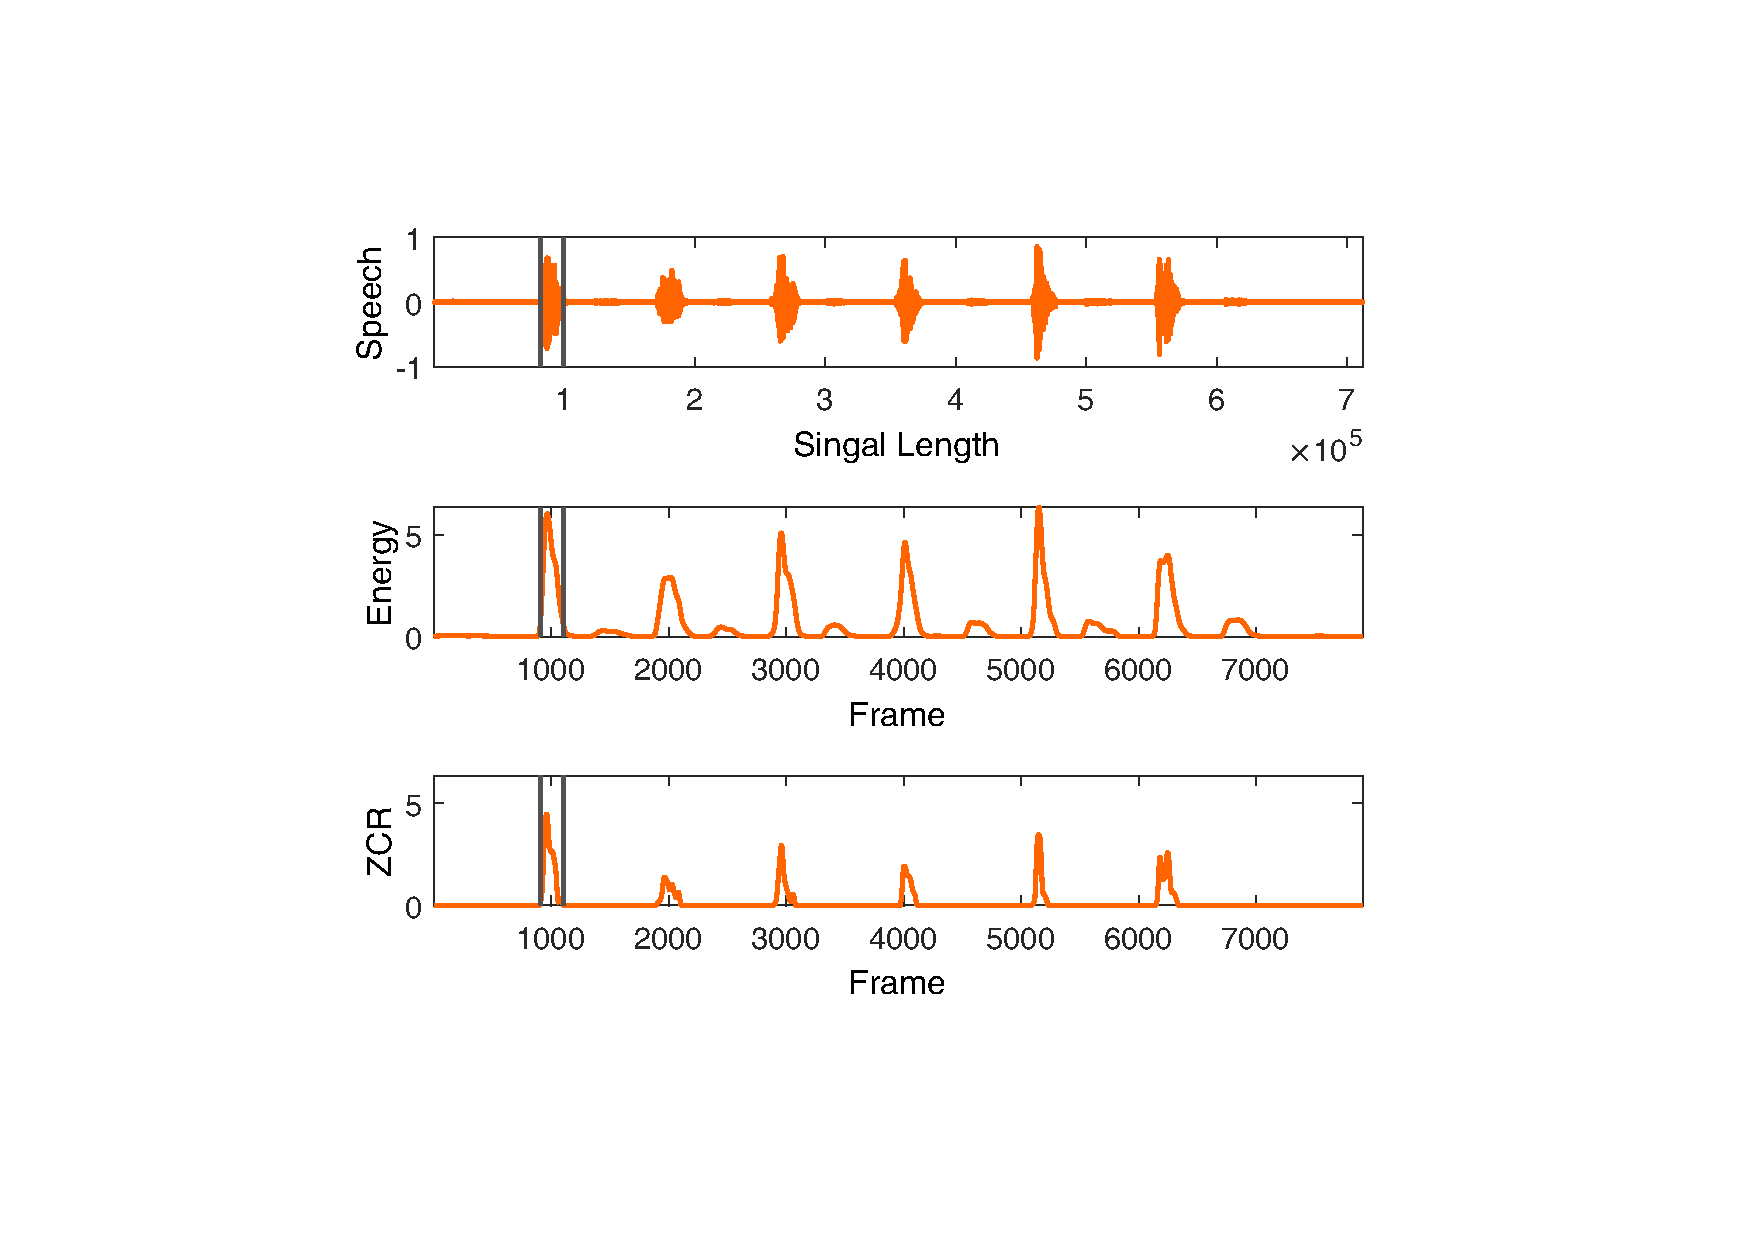
\includegraphics[width=0.32\linewidth]{Figures/snore.pdf}}
 \subfigure[Two consecutive cough.]{\label{cough}
   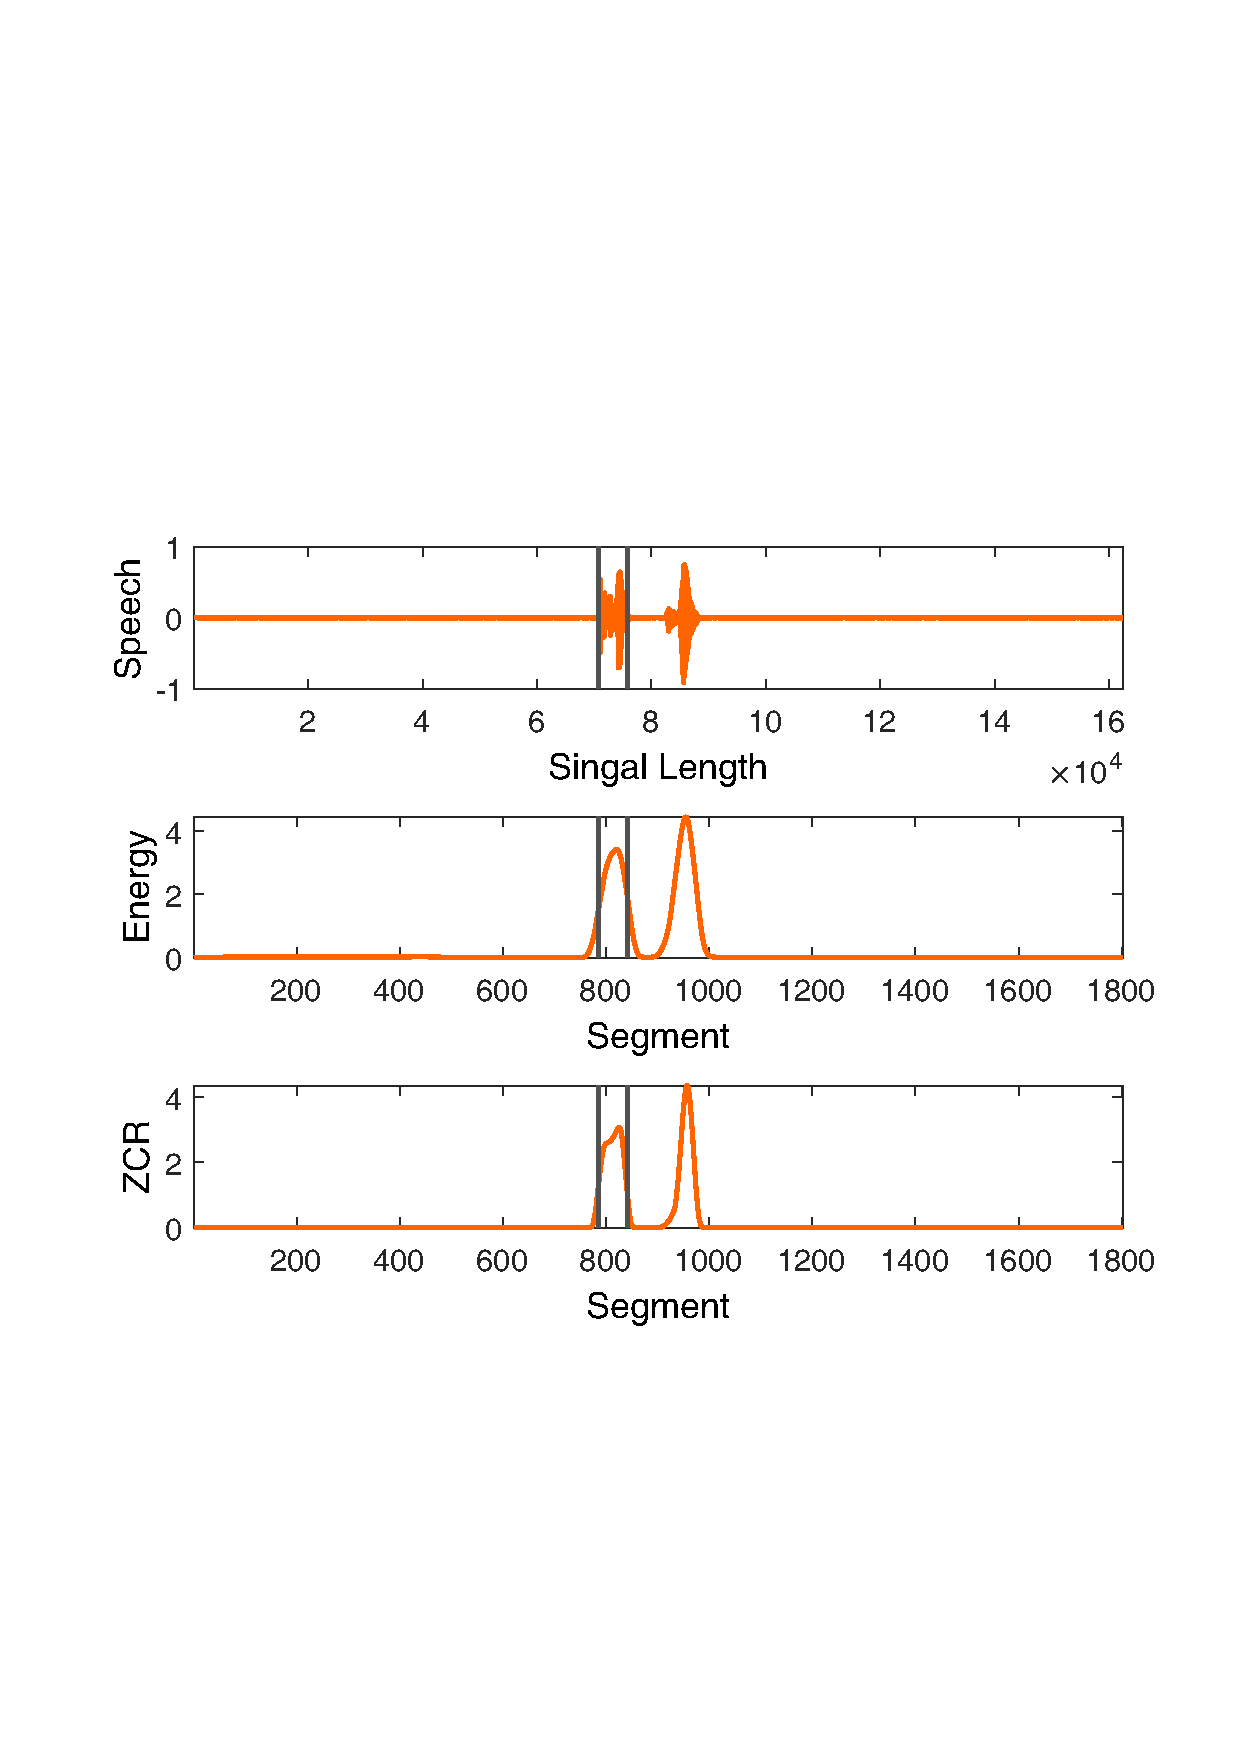
\includegraphics[width=0.32\linewidth]{Figures/cough.pdf}}
\subfigure[Somniloquy.]{\label{somniloquy}
     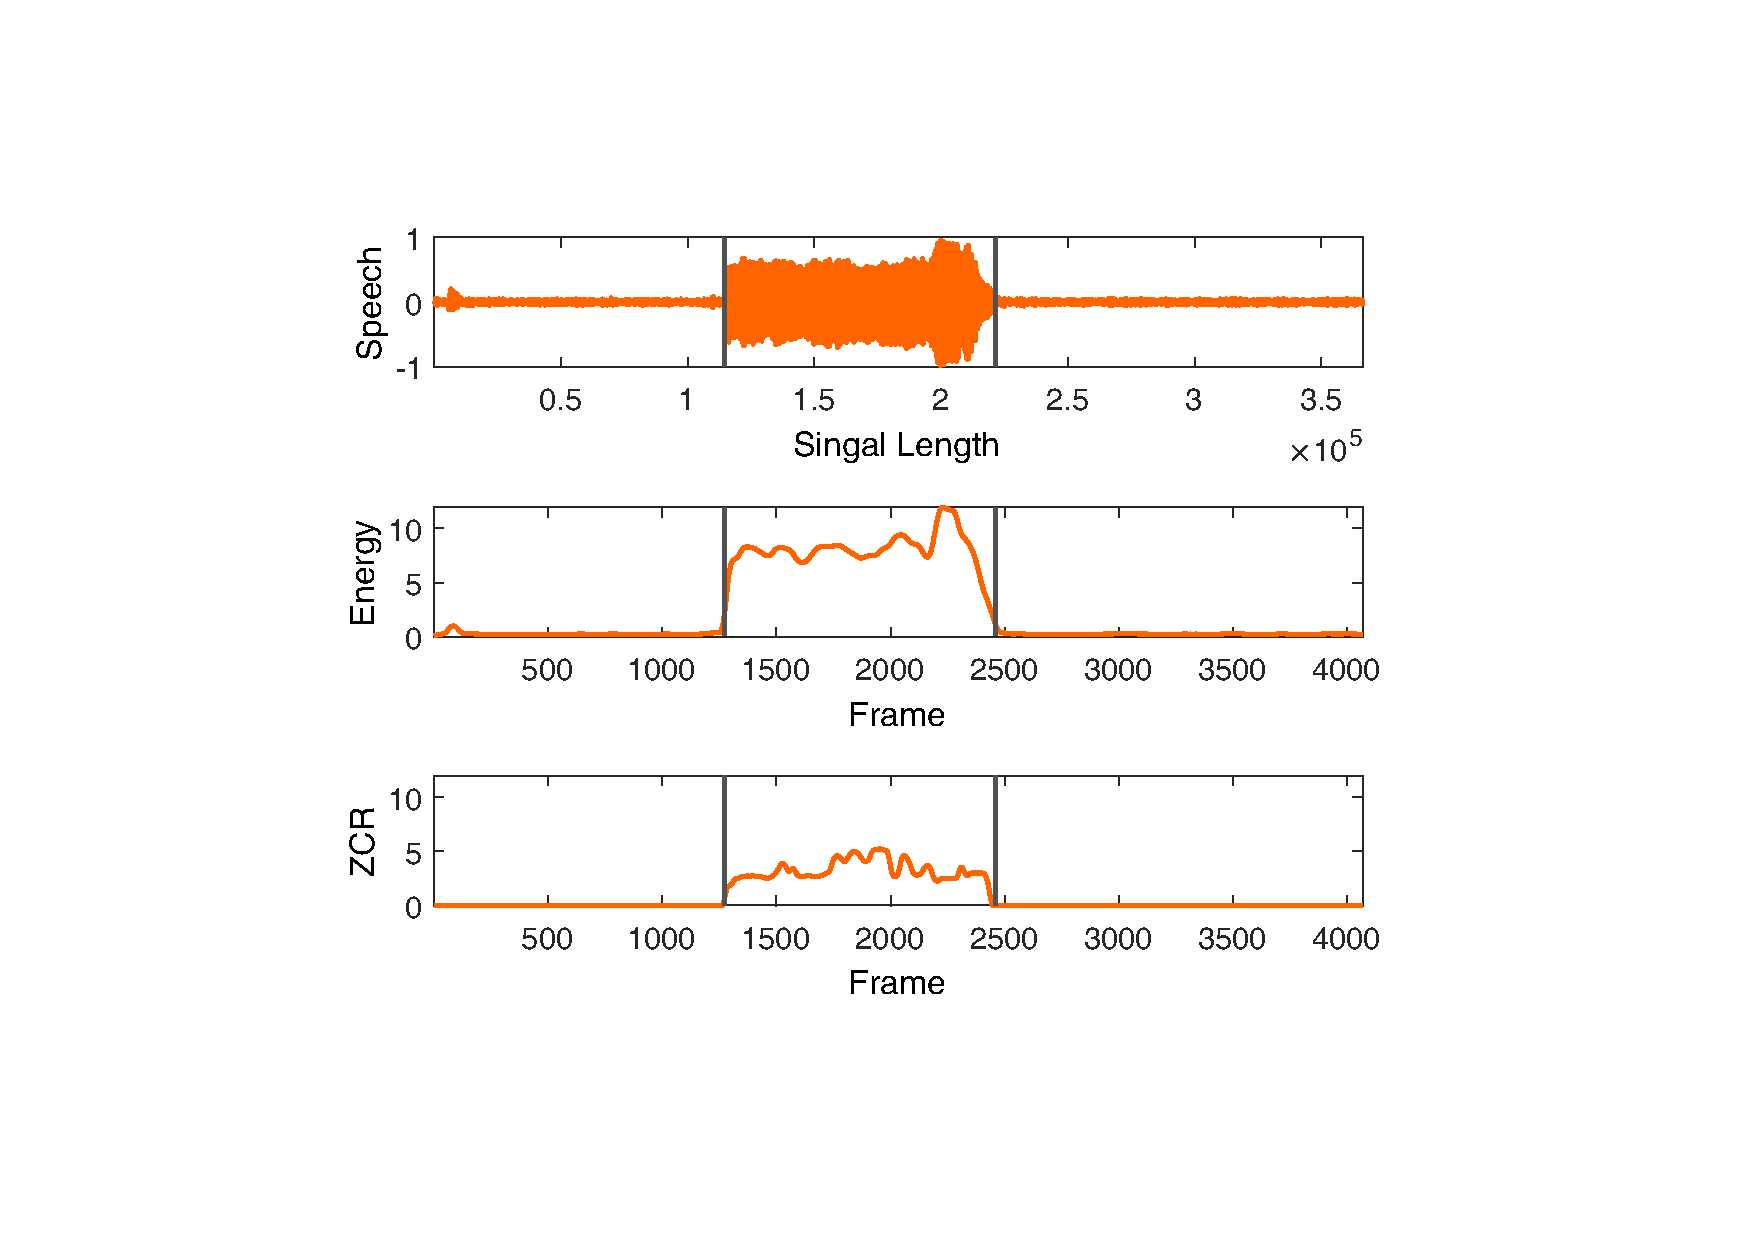
\includegraphics[width=0.32\linewidth]{Figures/somniloquy.pdf}}
\caption{The characteristics of different acoustic events.}\label{acoustic}
\end{figure*}


\subsubsection*{Acoustic feature calculation}
In order to identify different acoustic events accurately, we select the short-term average energy and the zero-crossing rate as two features. The short-term average energy of acoustic signal is computed as:
\begin{equation}
  E_i=\sum\nolimits_{j=-\infty}^{\infty}[x(j)\omega(i-j)]^2=\sum\nolimits_{j=i-(N-1)}^{i}[x(j)\omega(i-j)]^2,
\end{equation}
$N$ is the window length, $x$ is the signal and $\omega$ is the impulse response. As we can see that the short-term energy is the weighted
sum of squared frame sample. The short-term energy can be used to distinguish the segment of unvoiced and voiced sound. It also can be used
to differentiate speech segment and noise segment  in  case of relatively high signal to noise ratio (SNR). The zero-crossing rate is
computed as:
\begin{equation}
  Z_i = \frac{1}{2}\sum\nolimits_{j=0}^{N}|sgn[x_i(j)]-sgn[x_i(j-1)]|.
\end{equation}
It indicates the number of times, which the acoustic signal waveform passes through the horizontal axis (zero level). We carry out an interesting recognition experiment using the microphone built in smartwatch to detect the sound of people during sleep and effectively identify different acoustic events. We focus on three common acoustic events: snore, cough and somniloquy. Ten volunteers worn the smartwatches during sleep to record the acoustic data. We manually label the data with different acoustic events. Fig. \ref{acoustic} shows the acoustic characteristics of  three events. There are six times snore event, two consecutive cough event and somniloquy event.
%The sample rate is 22050 Hz.


\subsubsection*{Acoustic event recognition}
 At beginning, the algorithm  divides the audio stream into frames with equal durations. Each frame is composed of 256 samples, and its duration is 12 ms. To identify the  three common acoustic events, we introduce an acoustic recognition algorithm based on the following key observations:

 \begin{itemize}[itemsep=1mm,nolistsep]
\item The time interval between two signals for different acoustic events are quite different from each other. As shown in Fig.~\ref{snore}, there is a long time interval between two snores. While, the time interval between two coughs is very short.  In contrast, the  somniloquy signal is irregular and without periodic property.
    %Besides, the snore event produces periodic signals and their intervals  are similar.
 \item The duration of one signal for different acoustic events are different from each other. Fig. \ref{acoustic} shows that the duration of a snore is shorter than the duration of a cough and somniloquy. And in general, the duration of a cough is shorter than the duration of a somniloquy signal.
\item The frequencies for different acoustic events are quite different from each other. Snore event has a continuous signal, while the  cough and somniloquy are sudden events, thus the number of consecutive occurrences is very small.
\end{itemize}
In conclusion, the ``interval'', ``duration'' and ``frequency'' of acoustic events can be used as three unique features. Based on the above three observations, our acoustic event recognition algorithm involves the following two steps. First, in order to estimate the interval and frequency of an acoustic event, we perform the peak detection. We use the short-term average energy to calculate the peak value of the acoustic signal. When the peak exceeds a certain threshold, such as 3 dB in this paper, we record the position of each peak and calculate the interval between two consecutive peaks. Next, we can estimate the frequency of an acoustic event by counting the number of peaks over a time window. Second, to estimate the duration of the acoustic event, we perform the start-point and end-point detection.

Traditional end-point detection algorithm \cite{stowell2015detection}, however, uses a fixed double threshold and must be obtained by a
large number of data samples, which has two drawbacks. First, the fixed double threshold may cause error detection at the beginning of
acoustic event. Second, the requirement of a large number of data samples would lead to large system latency. To address
these issues, we develop a detection method that does not require pre-sampling to obtain the optimal thresholds. Instead, our algorithm
estimates the thresholds on a per signal basis. This strategy not only reduces the number of data samples needed, but also leads to a
higher accuracy.

Specifically, since the first few frames and the last few frames are mostly mute or are the background noise, we select the first five
frames and the last five frames to calculate their short-term energy, which are denoted as $E_s$ and $E_e$, respectively. And then the two
are combined to obtain the mean $E_n$ as the estimated energy value of the noise segment.Let the maximum value of the short-term energy
over all frames denoted as $\max (E)$. Then, the average short-term energy $DE$ is given as:
\begin{eqnarray}
      &E_n = \frac{(E_s+E_e)}{2}, \\
      &DE = \max (E)-E_n.\label{eq:DE}
\end{eqnarray}

So we can use $EH$ and $EL$ to represent the high and low threshold of short-term energy, which are given as:
\begin{equation}
      EH=\alpha \times DE+E_n,
\end{equation}
\begin{equation}
    EL=\beta \times DE+E_n,
\end{equation}
where $\alpha$ and $\beta$ are the multiplier factors of the energy value $DE$.


Here, we need to choose the right values for $\alpha$ and $\beta$ to ensure
 that we can accurately detect the start and end points of a speech signal. To that end, we use the night time sound data from our training dataset to determine $\alpha$ and $\beta$.
 Specifically, we tested $\alpha$ with values ranging between 0.1 and 0.5, and $\beta$ with values ranging from 0.01 to 0.09. We found that setting $\alpha$ to  0.1 and $\beta$ to  0.06 gives the best overall results in our training dataset.
 
To ensure sudden noise does not interfere with detection results, we set the minimum length of the signal segment and count the length of the signal during the search for the start and end point. Finally, if the signal length is less than the set minimum, it is considered as a noise segment. The results of the start-point and end-point detection are shown in Fig. \ref{acoustic}, we calculate the length of each speech segment and calculate their averages as the duration of the acoustic event. Last, we count the number of peak points to determine whether it meets the third key observation or not.



%Algorithm 1 provides the detailed  process of the start-point  and end-point detections.


%$A_x$, $A_y$ and $A_z$ are the tilt angle of the three axes, and $\omega_x$, $\omega_y$ and $\omega_z$ are the rotation speed of the three axes. So $\phi$, $\theta$ and $\psi$ are the rotation angle of the three axes. \textcolor[rgb]{1.00,0.00,0.00}{(Those symbols do not present in Algorithm 1)}


%\begin{table}[!thbp]
%\begin{tabular}{l}
%  \hline
%  \textbf{Algorithm 1} The Endpoint Detection \\
%  \hline
%  \textbf{Input}: A sound signal recorded by the microphone:$x$
%  \\\quad \quad \quad The threshold of zero-crossing rate:$ZT$
%  \\\quad \quad \quad The minimum length of speech:$minlen$\\
%  \textbf{Output}:The start-point  and end-point :$p_s,p_e$\\
%  1: Split  $x$ using the framing algorithm \\
%  2: Calculate each frame of energy and zero-crossing rate:$E_i,Z_i$ \\
%  3: Calculate the threshold for short-time energy:$EH,EL$  \\
%  4:$count=0$,$silence=0$\\
%  \textbf{the start point}\\
%  5:\textbf{for}i=1$\rightarrow \frac{length(x)}{frame~length}$  do\\
%  6: \textbf{if} $ E_i>EH $ \textbf{then}\\
%  7: $count=count+1$,$silence = 0$,$max(n-count-1,1)=p_s$\\
%  8: \textbf{else if} $E_i>El || z_i>ZT $\textbf{then}\\
%  9: $count=count+1$ \\
%  10: \textbf{else}\\
%  11:$count=0 $ \\
%  12: \textbf{end if}\\
%  \textbf{the end point}\\
%  13:\textbf{if} $E_i>El || z_i>ZT $\textbf{then}\\
%  14:$count=count+1$ \\
%  15:\textbf{else}\\
%  16:$silence = silence+1 $ \\
%  17:\textbf{if} $count < minlen$\textbf{then}\\
%  18:$count=0 $, $silence=0$ \\
%  19:\textbf{end if}\\
%  20:$count1 = count-\frac{silence}{2}$\\
%  21:$ p_e = p_s + count1 -1$ \\
%  \hline
%\end{tabular}
%\end{table}


\subsection{Tracking Illumination Conditions \label{sec:illumination}}
Studies have shown that there is a significant interaction between illuminance level and the mental state of the individual \cite{light77}.
For example, the bright light can counteract subjective fatigue during daytime, but at night it will seriously affecting the sleep quality.
Too much light exposure can shift our biological clock, which makes restful sleep difficult to achieve, it affects our sleep and wake cycle
\cite{light2007}.  Besides, we also note that the dim light will affect our sleep too. According to the study \cite{light2016}, it can be
learned that the dim artificial light during sleep is significantly associated with the general increase in fatigue, and the proper light
can be used to increase the sense of exhaustion and promote sleep. So illumination condition in a sleeping environment has a significant
influence on sleep. {\systemname} use the ambient light sensor to detect the illumination condition during sleep. We visit the bedroom of
our ten testing users at night and the use of the ambient light sensor to test the lighting conditions in the bedroom. We
find that in the absence of lights in the bedroom, the light sensor reading is between 1 Lux to 4 Lux. In some cases, the light of the
smartwatch screen can raise the light sensor reading to 4 Lux when the bedroom is dark. In other cases, when the bedroom has weak lights
(e.g., when the bedroom is illuminated using a table lamp), the light sensor's average readings are below 10 Lux. Based on these
observations, we divide the illumination intensity of the bedroom into two categories. When the bedroom has weak lights (i.e., the light
sensor reading is no greater than 10 Lux), and when the bedroom has strong lights (i.e., the light sensor reading is greater than 10 Lux).
Using the threshold of 10 Lux, we can then map the light sensor readings to one of these two groups.


However, the light sensor may be obscured, which leads to large errors in measuring the illumination level. For example, a user's
smartwatch may be covered under quilt when he/she turned over unconsciously, and thus the illumination readings on the smartwatch may not
reflect the real lighting situation. Most of the previous works on smartphone-based light detection have used the proximity sensor
to detect whether the light sensor is blocked or not. However, such an approach is not applicable to the off-the-shelf
smartwatches because they typically do not have a proximity sensor.  To deal with this practical challenge, the key is that the
illumination would drop suddenly when the smartwatch is covered by other objects. There are two possibilities for the sudden drop in light
intensity. For most smartwatches, the light sensors are usually installed in the front face of it. The first case is the indoor lighting
facilities are closed. The second case is the wrist turned so that the back of the hand become downward, thus blocking the light sensor in
front of the smartwatch. Such a situation often happens in real life. For examples, when a user changes the sleeping
posture to the left side, his/her hand may be close to the pillow with the palm facing up; or the back of the hand may become downward
because of a hand movement. To avoid this erroneous illumination condition measurement, we detect whether the user is performing a wrist
flip over a period of time during the intensity plummeting. We detect the wrist flip based on two aspects: (i) the rotation angle of
smartwatch; (ii) whether the light intensity maintains stable after the sharp drop. If the wrist flips, we use the average of the previous
light intensity as the intensity of the time period. It should be noted that, because the illumination condition detection algorithm is
relatively simple, it is not explained in the experimental part.

\subsection{Sleep stage and quality}

Sleep is generally considered as a cyclical physiological process composed of three stages: rapid eye movement (REM) stage, light sleep stage and deep sleep stage. REM is an active period of sleep marked by intense brain activities and dream occurrence. Light sleep stage is a period of relaxation, when the heartbeat, breathing rate and muscle activity slow down. Deep sleep stage triggers hormones to promote body growth, as well as the repair and restoration of energy.  The biological characteristics of different sleep stages exhibit distinguishingly. In clinical sleep study, the sleep stages are mainly identified by simultaneously evaluating three fundamental measurement modalities including brain activities, eye movements, and muscle contractions. The EEG measure using electrodes placed around the scalp interpret various sleep/wake states of the brain. And, EMG and EOG using electrodes placed on the skin near the eyes and on the muscles, respectively, measures in deeply differentiating REM stage from all the other stages. But, apart from the implicit physiological activities, sleepers usually exhibit distinguishable physical activities in different sleep stages. For example, there are somniloquy and body trembles caused by frequent dreams generally appear in REM, large body movements such as body rollovers and arm raising happen in light sleep and micro body movements such as body trembling and snoring occur in deep sleep.  In the meanwhile, the breathing amplitude in NREM stage is larger compared with the REM stage. Moreover, sleep cycle usually repeats four to six times over a night. The sleeper usually experiences a transition from light sleep to deep sleep and then enters REM, but sometimes there is also possible a phenomenon of skipping some certain sleep stages occurs during sleep. However, despite this, dependence between two successive sleep stages still exists and different sleep stages have potential conversion probabilities, which also mentioned in Sleep Hunter \cite{gu2016sleep}.

To separate between these states, we build a Hidden Markov Model~\cite{johnson2010hidden} for identifying the current sleep stage of the user. As the input, i.e., the observed states, we use series of detected sleep events and the sleep stage sequence is modelled as a hidden state, i.e., $obs_t={NB(t),NB_M(t),BA(t),NA(t)}$ represents the feature vector at detection phase t. The explanation of each item, which is the input of HMM, is listed as follows. $NB(t)$: the number of occurrences of body rollover during the detection phase t. $NB_M(t)$: the number of occurrences of micro body movement. $BA(t)$: the measurement of respiratory amplitude. $NA(t)$:the number of occurrences acoustic events. And $states_t$ =$\{$light sleep; deep sleep; REM$\}$ is an output of our model, which represents the sleep stage in the detection phase t. In the training of the HMM model, we used nocturnal sleep data from 10 volunteers who participated in the training parameters of each algorithm and make their sleep-related events as observation sequences and the corresponding sleep stages detected by Fitbit as hidden state sequences, to generate HMM models. Specifically, we first use maximum likelihood estimation method for parameter estimation, the state transition matrix and the confusion matrix, and then use the Viterbi algorithm to acquire a series of implicit state sequences corresponding to observed sequence.  As a result, we can estimate the sleep stage during a time window. Finally, we can get the durations of all sleep stages over the whole sleep process.

Further, to quantize the quality of a sleep, we use the Sleep Quality Report model introduced in \cite{gu2016sleep}. Let $SQ$ be the value of the sleep quality, then $SQ$ is given as follow:
 \begin{equation}
SQ=\frac{(REM \times 0.5+Light \times 0.75+Deep) \times 100}{REM+Light+Deep}
 \end{equation}
where, REM, Deep and Light represents the duration time in a sleep process. The range of $SQ$ is from 50 to 100. A high value of $SQ$ shows a good  sleep quality.


\section{EVALUATION METHODOLOGY}\label{sec:expsetup}


\begin{figure}[!t]
	\centering
	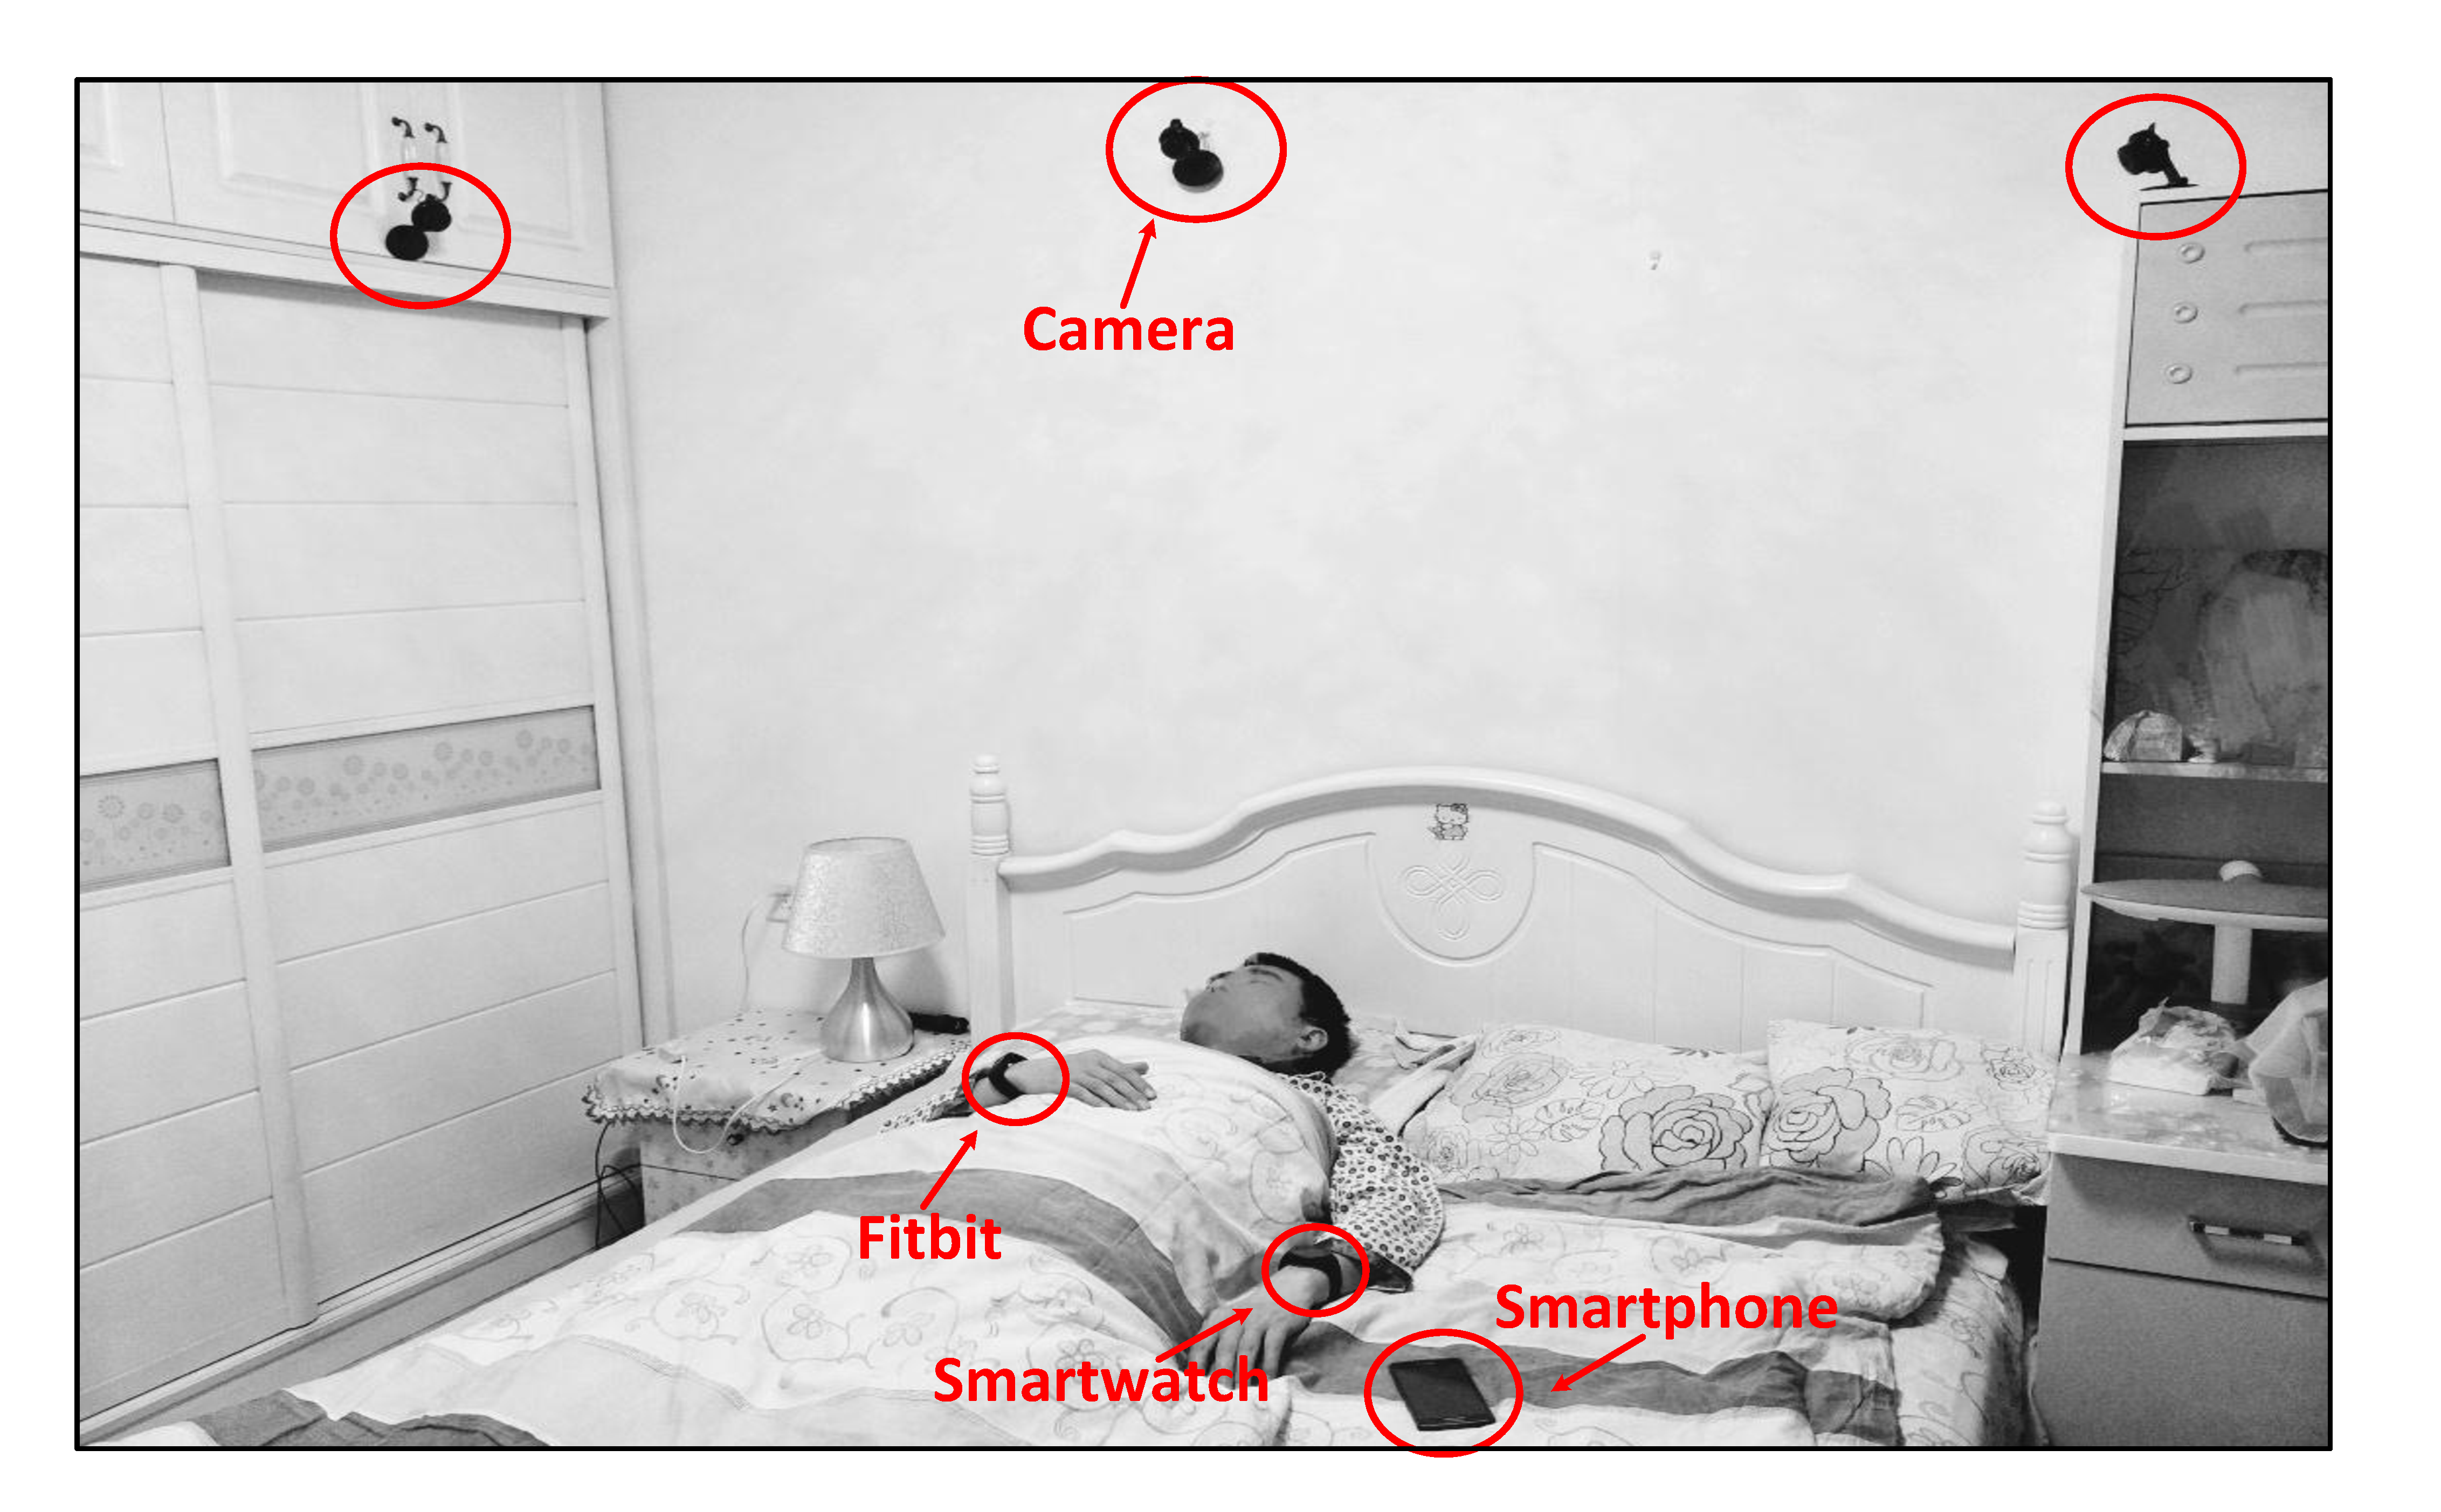
\includegraphics[width=0.57\linewidth]{Figures/setup.pdf}
	\caption{Experimental setup in one of our participants' home. }\label{fig:setup}
\end{figure}



\subsection{Experimental Setup\label{sec:evalusers}}

We evaluate {\systemname} through experiments conducted in $15$ single-occupancy homes over a two-week period.  The participants include 6 males and 9 females, whose age spans 15 to 60 years. To ensure too little sleep had no effect on the results, each participant was required to sleep at least $6$ hours per night during the study period. Two of our participants have been diagnosed with long-term, on-going sleep-related disorders, and one participant has described that his sleep is significantly affected by snoring. The remaining participants reported their sleep quality to go up and down. The study was approved by local IRB, and participants were separately asked to consent to release their data for analysis. In total, we collected 210 sets of nocturnal sleep data from our participants.

During the study, participants are asked to wear a smartwatch on their wrist. To obtain ground truth of sleep events, three video cameras were placed on the ceiling to monitor the user's sleep activities, as shown in Fig.~\ref{fig:setup}. The cameras have night vision and thus can capture sleep activity with high-quality. The video footage was manually labeled with different sleep activities and the labels were used as ground truth in our evaluation. Specifically, we consider the respiratory amplitude during the NREM stage as large amplitude, and the one during REM stage as normal amplitude. For the acquisition of sleep stage information, we confirm labels when both Fitbit and {\systemname} reach a consensus. To demonstrate the overall benefits of {\systemname} and the events captured by it, we separately collected ground truth information about sleep quality using questionnaires which were administrated each morning. The questionnaires were based on the Pittsburgh Sleep Quality Index (PSQI), a widely used and validated questionnaire in sleep quality research~\cite{buysse1989pittsburgh}. Finally, we collected sleep stage estimates from a Fitbit Charge2 and considered them as ground truth for sleep stage estimation. While the performance of Fitbit is not comparable to medical grade PSG, it has been shown to have a good association in adults~\cite{evenson2015systematic,fitbit01,fitbit02,fitbit03}, especially in estimating REM and light sleep stage. Equipping the participants with PSG was not feasible as it would disrupt their normal sleeping routines and potentially bias and reduce sleep activities, which are the main focus of our work. Moreover, the goal of our experiments is not to demonstrate that {\systemname} is capable of medical-grade sleep monitoring, but to demonstrate that it performs comparably to commercial systems in common sleep monitoring tasks, while at the same time being able to capture a much richer set of sleep information. We also compare our approach against Sleep Hunter~\cite{gu2016sleep}, a state-of-the-art mobile-based sleep monitoring approach, and a smartphone-based sleep monitoring app named Sleep as Android~\cite{SleepAndroid}. To provide a fair comparison against these baselines, we also place a smartphone next to the user's body on the bed to collect the data for Sleep Hunter and Sleep as Android.
	

\subsection{{Pilot Study: Training Data}}\label{sec:trainingdata}

Prior to our main study, we carried out a pilot study that was used to inform our algorithm design, and to provide training data for the algorithms integrated into {\systemname}. Our pilot study consisted of two groups (aged ranged from 15 to 60). One group \nt{consisted of} randomly selected 100 volunteers to conduct questionnaire surveys to provide the basis for our algorithm design. The other group consisted of 10 users whose data was used to train our models.


To improve the effectiveness of the algorithms integrated into {\systemname}, especially sleep posture and hand position detection, we elicited questionnaires to 100 volunteers to identify their common sleep posture. The main content of the questionnaire was about their common arm position in the four basic sleeping postures. Based on this investigation and previous research~\cite{position2014,HandPosition2}, we selected the positions to consider in {\systemname}. We also found that these arm positions are effective during the training and testing of the algorithm.

To train the models used in our system and to determine optimal parameter values, a small-scale pilot study with $10$ participants was carried out prior to the main experiment. The training examples used to train our algorithms and to determine the algorithm parameters are collected from 10 users (5 males and 5 females). Our testing users were asked to wear a smartwatch to sleep and collected the sensor data while they were sleeping. Every testing user contributes 10 nocturnal sleep data over a two-week period. These users were different from those taking part in our evaluation (Sec.~\ref{sec:evalusers}).



\subsection{Prototype Implementation \label{sec:implementation}}
We prototype and evaluate {\systemname} on a Huawei Smartwatch 2 wearable device. The smartwatch is equipped with a Quad-core Cortex-A7 processor at 1.1 GHz. It runs the Android Wear 2.0 operating system. We use five sensors of the smartwatch: the accelerometer, gyroscope, microphone, light sensor and orientation sensor. To reduce the energy consumption of the smartwatch, in the experiments we analyze the sensor data on a XiaoMI Note2 Android smartphone to which the smartwatch sends sensor measurements over Bluetooth. The sensors on the smartwatch are sampled every $30$ms, which was chosen to balance between information quality and energy consumption. {\systemname} starts tracking sleep events when it detects that the light is off and there has been nobody movement for 30 minutes. As part of an initialization process, {\systemname} estimates the initial body posture and hand position. It then uses these as a starting point to monitor sleep events like the body posture, rollovers, hand positions and body movements.

\section{RESULTS}\label{sec:4experiment}
In this section, we detail the evaluation results for our system.

\subsection{Evaluation of Subcomponents}
We focus on the detection accuracy about five events, that are body posture, the body rollover, the hand position, the micro body movements and the acoustic events.

\subsubsection{Sleep posture classification performance}
\label{subsub:bodyposture}

We first test the overall classification performance of different body postures. The ground truth of body postures is recorded by the cameras. To avoid biases in the evaluation, and to assess the generalization performance of our approach, we consider a cross-validation scheme where all data from a single participant is used for training and data from the remaining $14$ participants is used for testing. The motivation for using data from a single user as training data is to highlight the capability of {\systemname} to accurately characterize body posture with very little training data, while at the same time being able to generalize across users. The final performance is then calculated as the averaged accuracy across the 15 folds; as shown in Fig.~\ref{fig:posture_zhu} and Table \ref{tab:posture}. We can observe that the posture detection accuracy is consistently high across all users, and does not show major variations across users. This good performance benefits from the distinct characteristics of arm position under different sleeping postures. Compared to results reported for SleepMonitor~\cite{sleepmonitor}, {\systemname} consistently improves performance which is mainly due to the template-based classifier that we use to verify classifications of the prone and supine states. In particular, {\systemname} achieves around $5$ percentage units higher performance on the prone state than SleepMonitor and overall has a lower false positive rate. In addition, {\systemname} considers more hand positions than SleepMonitor in 4 sleeping postures. In terms of errors, due to angular characteristics of acceleration being similar between the supine posture with the hand putting on the head and the left-lateral posture, a small amount of the supine postures are classified as left lateral. From the results, we can also observe that the total amount of the prone posture is smaller than the number of other postures, which suggests that people are not accustomed to sleeping in this position because it is neither healthy nor comfortable.

\begin{figure}
	\centering
	\begin{minipage}{.5\textwidth}
	 \centering
	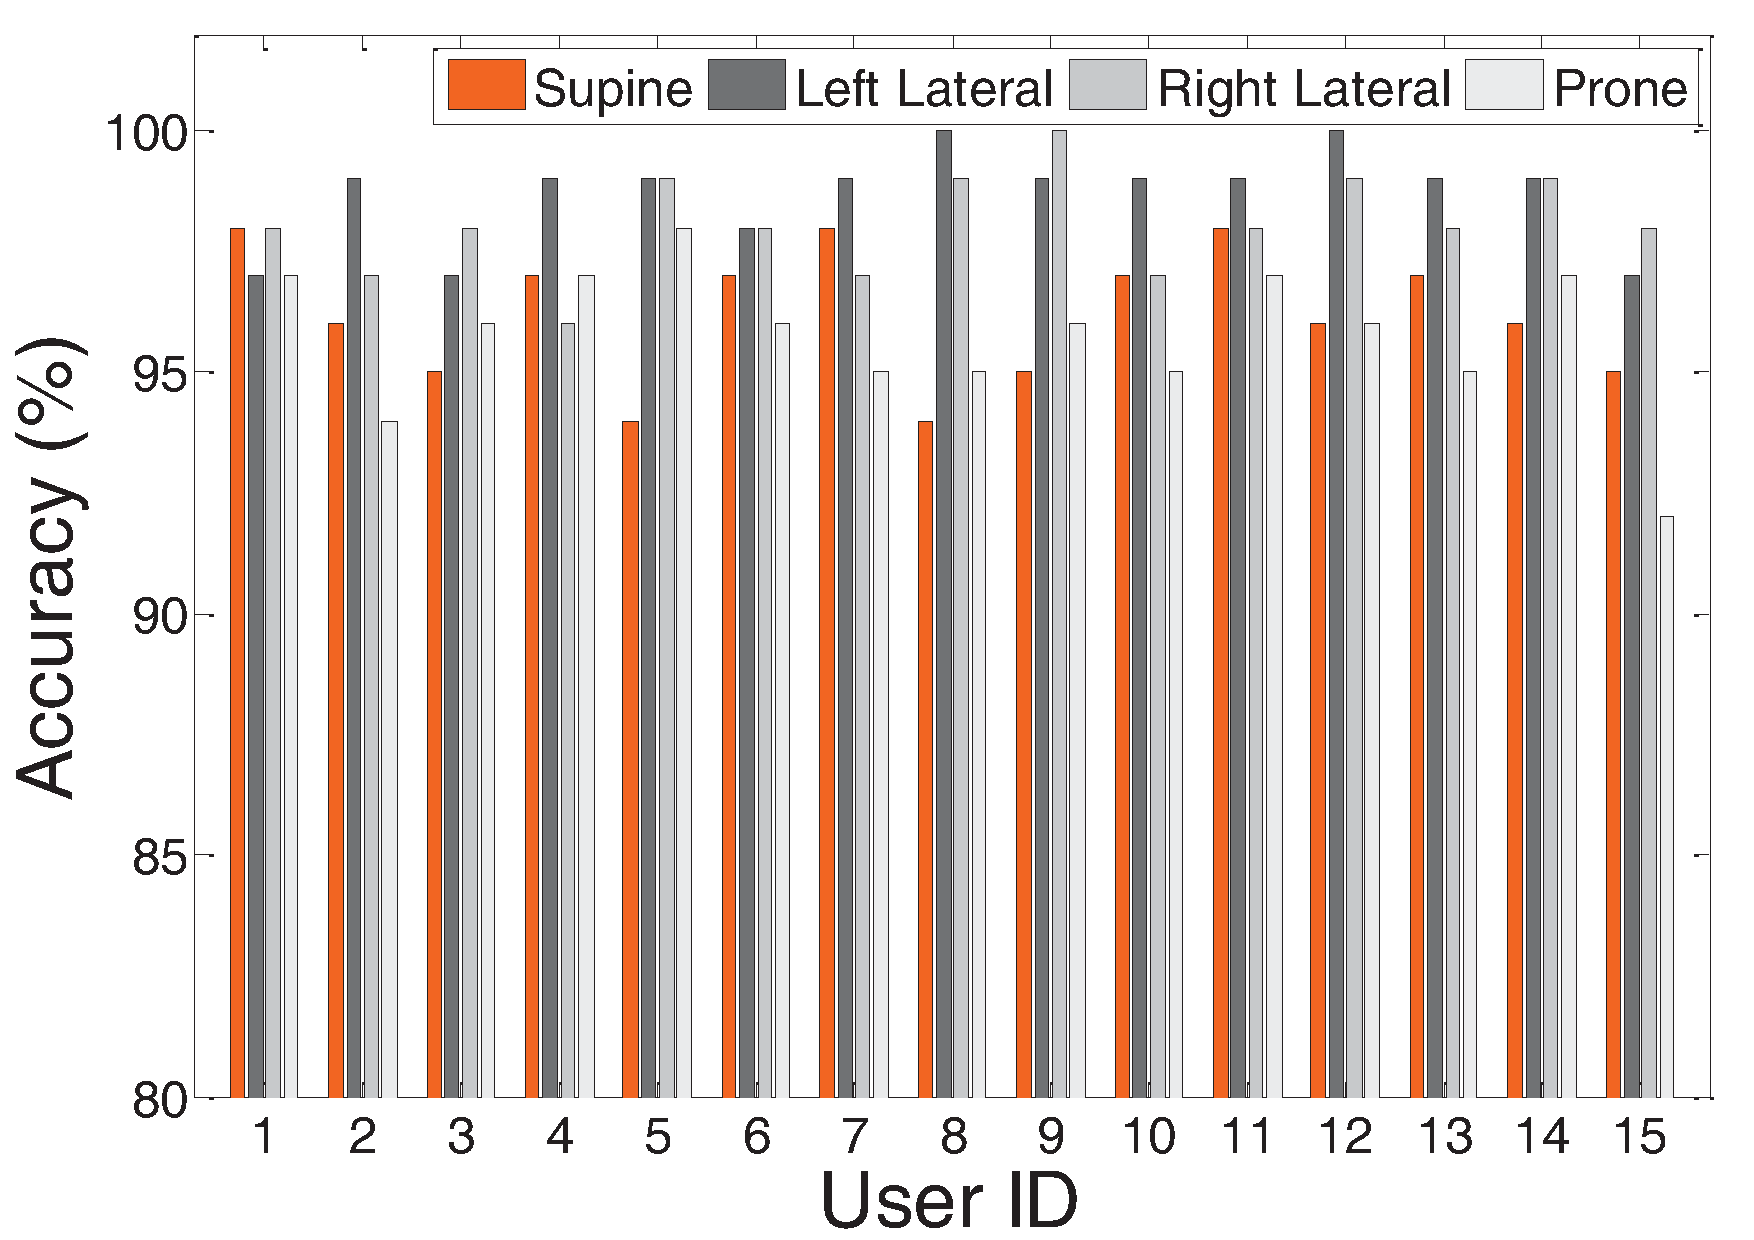
\includegraphics[width=0.95\linewidth]{Figures/posture_zhu.pdf}
	\caption{Detection accuracy of body postures.}\label{fig:posture_zhu}
	\end{minipage}%
	\begin{minipage}{.5\textwidth}
			\centering
		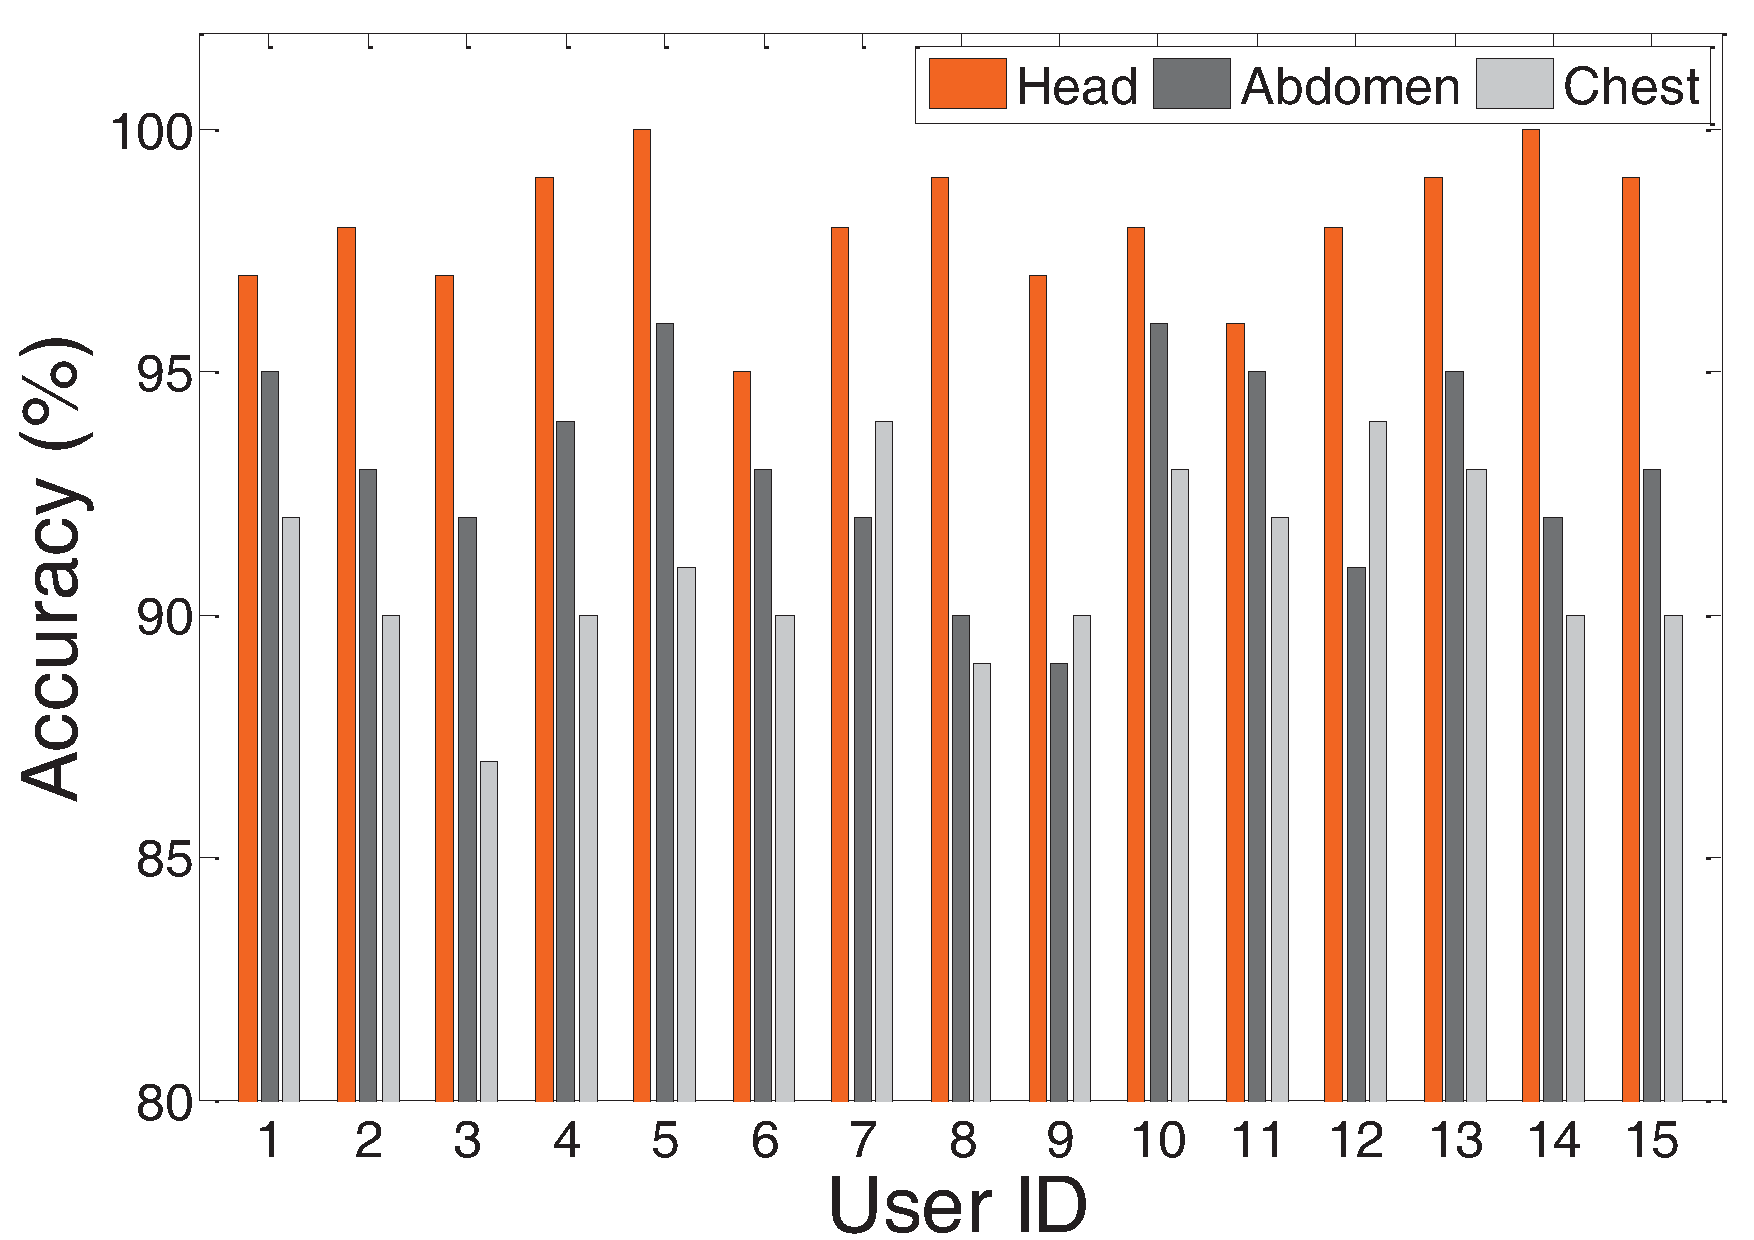
\includegraphics[width=0.95\linewidth]{Figures/handposition_zhu.pdf}
		\caption{Identification accuracy of hand positions.}\label{fig:hand_zhu}
	\end{minipage}
\end{figure}

\begin{table}[!t]\footnotesize
	\centering
	\renewcommand\arraystretch{0.3}
	\caption{The confusion matrix of body posture classification.}\label{tab:posture}
	\begin{tabular}{c| c | c | c | c | c | c}
		\cline{1-7}
		&\multicolumn{1}{ c|}{ }
		& \multicolumn{4}{ c|}{ }\\
		\multirow{2}*{}
		&\multicolumn{1}{c|}{\multirow{2}*{{Result}}}
		&\multicolumn{4}{c|}{{Prediction}}
		& \multirow{4}*{{Recall}} \\
		\cline{3-6}
		& & & & & \\
		\multicolumn{1}{c|}{{}}
		&  \multicolumn{1}{c|}{{}}
		&  \multicolumn{1}{c|}{{Supine}}
		&  \multicolumn{1}{c|}{{Left Lateral}}
		&  \multicolumn{1}{c|}{{Right Lateral}}
		&  \multicolumn{1}{c|}{{Prone}}   \\
		& & & & & \\
		\cline{1-7}
		& & & & & \\
		\multirow{5}{*}{\begin{sideways}{{Groundtruth}}\end{sideways}}
		&   {Supine}   & {\bf{{1182}}}    &   $25$      &   $4$      &   $9$    &   {96.7\%}\\
		& & & & & \\
		\cline{2-7}
		& & & & & \\
		&   {Left Lateral}   &   $6$      &   {\bf{{1292}}}     &   $0$      &   $0$   &   {99.5\%} \\
		& & & & & \\
		\cline{2-7}
		& & & & & \\
		&   {Right Lateral}   &   $7$      &   $0$      &  {\bf{{1275}}}      &   $12$  &   {98.5\%}  \\
		& & & & & \\
		\cline{2-7}
		& & & & & \\
		&   {Prone}   &   $19$      &   $2$      &   $3$      &   {\bf{{567}}}   &   {95.9\%} \\
		& & & & & \\
		\cline{1-7}
		& & & & & \\
		&   {Precision}    &   {97.3 \%}   &   {98.0\%}   &   {99.5\%}   &   {96.4\%}    \\
		& & & & & \\
		\cline{1-7}
	\end{tabular}
\end{table}


\subsubsection{Performance of body rollover counting}
To verify the efficiency of body rollover detection algorithm, we compare each user's body rollover events detected by {\systemname} against the data labeled by watching the video. The performance is shown in Table \ref{tab:rollver}. We can see that User 3, User 4 and User 13 have an unusually high number of rollovers. For User 3 and User 4, they have difficulty in falling asleep due to the sleep disorder. User 13 needs to rollover frequently because of his loudly snoring. As we demonstrate in Sec.~\ref{sec:user_survey}, these participants also suffered from poor sleep quality and hence indicate how the information extracted by {\systemname} can support the detection of sleep problems. For all the 15 users, the detection accuracies are all very high, and the lowest one is still 87\%. Thus {\systemname} can accurately distinguish the large hand movement from the body rollover in bed. Moreover, detecting errors in body rollover events will not have a significant impact on our end result, because the division of sleep stages is a comprehensive consideration of all the detected features in each stage, such as micro body movement and acoustic events.

\begin{table}[!thbp]\footnotesize
  \caption{Detection accuracy of body rollover.}\label{tab:rollver}
   \renewcommand\arraystretch{1}{\multirowsetup}{\centering}
        \begin{tabular}{cccccccccccccccc}
        \toprule
         \textbf{Testing User ID}    & 1& 2  & 3& 4& 5& 6& 7& 8& 9& 10& 11& 12& 13& 14& 15\\
        \midrule
             {Labeled \#body rollover}  &231&204&442&397&198&101&196&164&193&208&131&205&342&149&156 \\
                 { Accuracy} &91\%& 94\% &88\%&93\%&96\%&94\%&87\%&90\% &93\% &94\% &92\% &94\% &89\% &90\% &95\%\\
        \bottomrule
 \end{tabular}
\end{table}

\subsubsection{Performance of hand position recognition}
To test the recognition performance of different hand positions, we consider the same cross-validation scheme used for body posture detection, i.e., one user's data is used for training the classifier and the remaining 14 users' data as test data. The classifier for detecting the hand movement trajectory is combined with the detection of periodic signals caused by respiration, then the hand position on the chest (or abdomen or head) can be identified. In our dataset, 14\%, 36\% and 22\% of the time the hand in the supine posture during sleep were placed on the head, abdomen, and chest respectively. Fig.~\ref{fig:hand_zhu} illustrates the accuracy of hand position across 15 users. As we can see that with just one set of training data, the accuracies for different users are all higher than 87\%. Therefore, our system can achieve a good identification accuracy for different hand positions. Moreover, we find that at least four out of fifteen participants tend to put their hands on their heads; one participate unconsciously puts his hand on his chest which makes him have nightmares. Those are all bad habits disrupting a good sleep. {\systemname} can report such key findings to improve the users' sleep qualities.


\subsubsection{Performance of micro body movement detection}

To assess the detection accuracy of micro body movements, we manually label the ground truth recorded by the camera during sleep, including hand moving, arm raising, and body trembling. We also use the accelerometer embedded in the smartphone which placed on the bed to record the occurrence of micro body movements, so as to avoid missing some movements such as trembling concealed by the duvet. For the acceleration data collected by smartphone, we first smooth the acceleration along the three axes, calculate Root Sum Square (RSS) to merge them and obtain the first-order derivative of the merged acceleration. And then we use the threshold detection method to mark the occurrence of motion. Since body trembling is the easiest to be covered, we only focus on such events. So we use a smartphone to detect the occurrence of events and the classification of the event is not performed. Table~\ref{tab:micro_move} list the total number of three micro body movements for each user over the testing period of 14 days, and Fig.~\ref{fig:micro_movement_zhu} reports the accuracy of {\systemname} for detecting these micro body movements. It shows that the accuracies for all users are very close, that is, there will be no major changes between users. And from Fig. \ref{fig:micro_combine}, we find that even though the worst classification result belongs to the hand movement, the average precision value and recall value still exceed 75\%. The averaged accuracies of arm raising and body trembling are 93\% and 84\%, respectively. Because the training data volume for the hand movement and body trembling is small, so the performance can be improved by setting each user a threshold by collecting a longer term's sleeping data. In addition, the purpose of micro body movement detection is to detect different sleep stages, and the hand movement usually appears in all sleep stages, thus the poor accuracy of hand moving does not have a significant impact on the final result.


\begin{figure*}
	\centering
	\begin{minipage}{.485\textwidth}
		 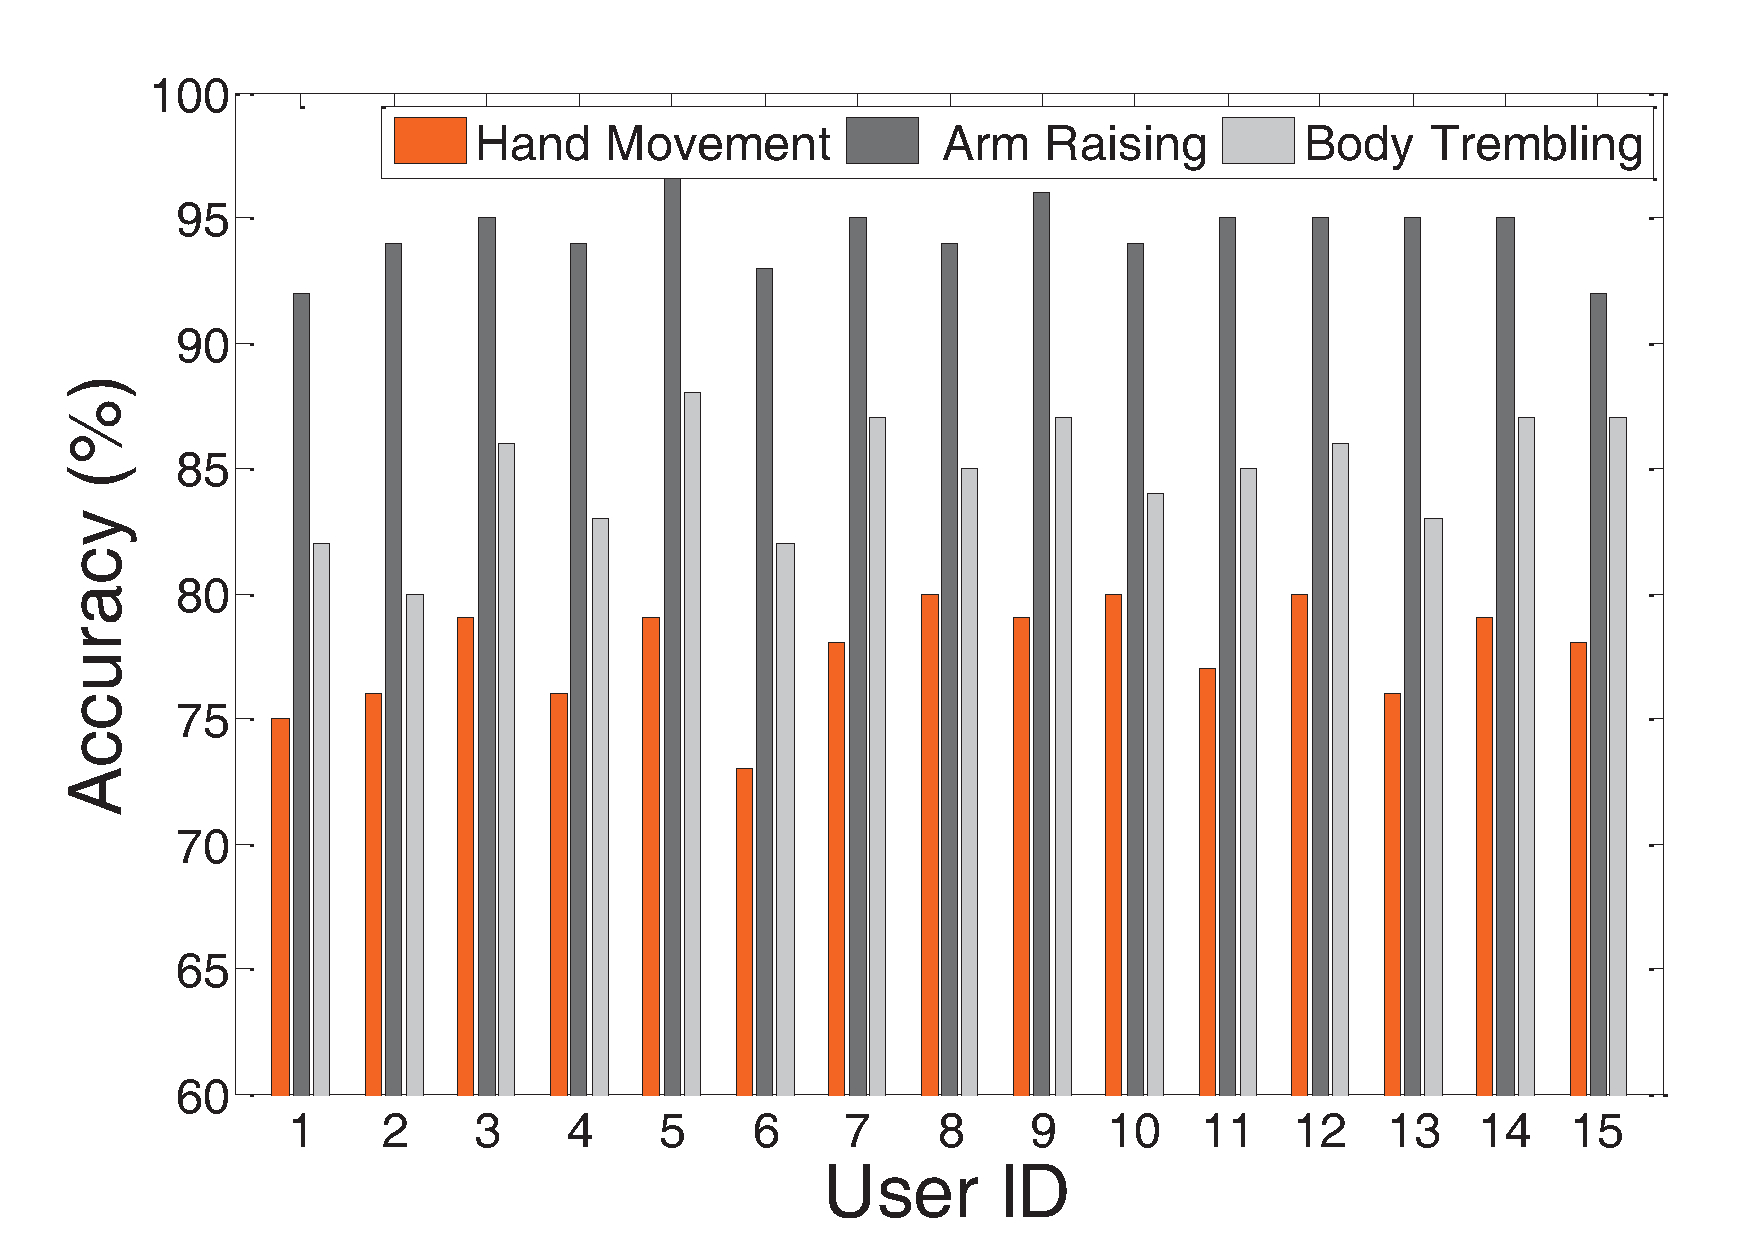
\includegraphics[width=0.95\textwidth]{Figures/micro_movement_zhu.pdf}
		\caption{Micro body movement detection accuracy for each user.}\label{fig:micro_movement_zhu}	
	\end{minipage}%
\hspace{3pt}
	\begin{minipage}{.485\textwidth}
	 \centering
	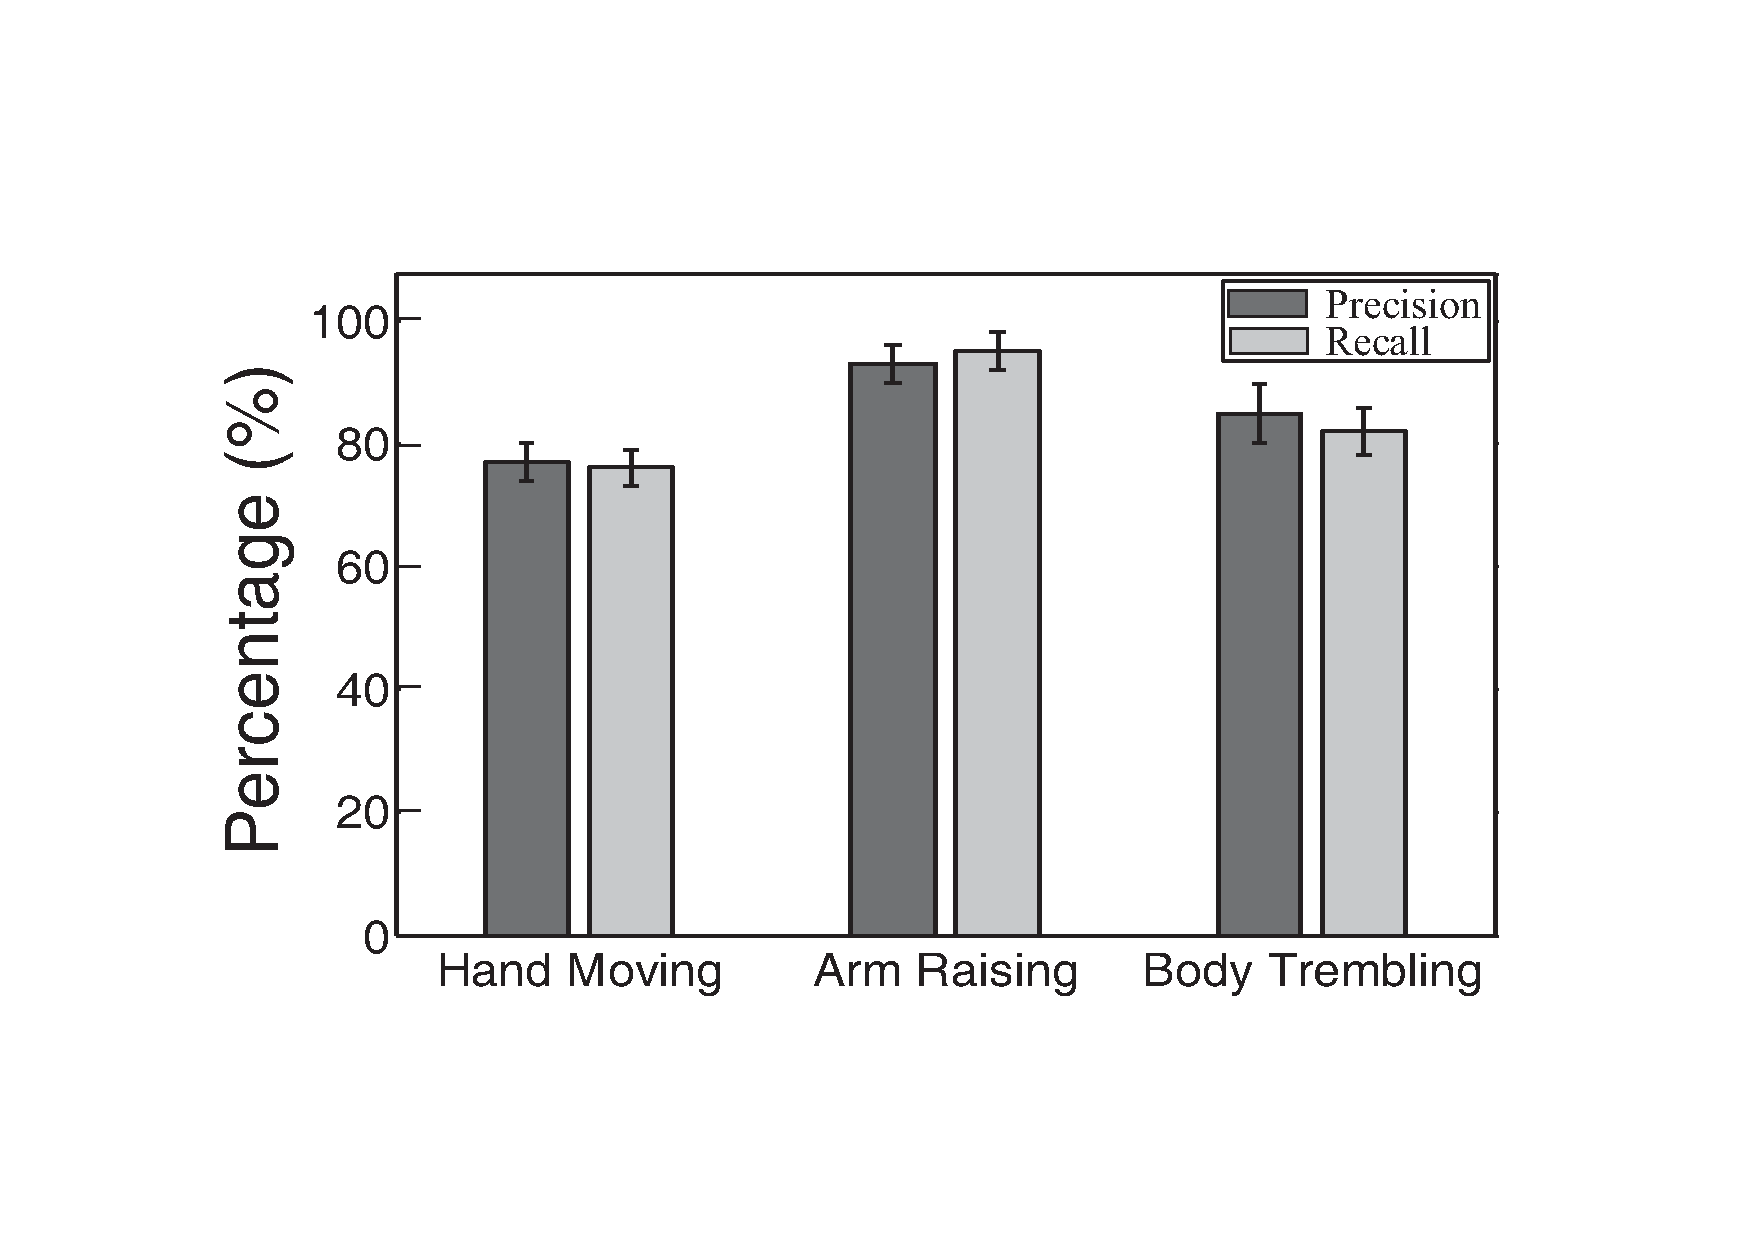
\includegraphics[width=7.8cm,height=5cm]{Figures/micro_combine1.pdf}
	\caption{Average precision and recall for micro body movement detection.}\label{fig:micro_combine}
	\end{minipage}
\end{figure*}


\begin{table}[!t]\footnotesize
  \caption{The number of micro body movements per user.}\label{tab:micro_move}
   \renewcommand\arraystretch{1}{\multirowsetup}{\centering}
        \begin{tabular}{lccccccccccccccc}
        \toprule
         \textbf{Testing User ID}    & 1& 2  & 3& 4& 5& 6& 7& 8& 9& 10& 11& 12& 13& 14& 15\\
        \midrule
            \rowcolor{Gray} {Labeled \#hand movement}  &52&49&67&55&78&65&59&70&61&53&81&55&60&59&63 \\
             { Labeled \#arm raising} &48&50&62&53&66&49&57&50&73&45&54&69&57&56&61\\
             \rowcolor{Gray} { Labeled \#body trembling} &28&32&25&29&34&25&20&30&24&26&27&35&24&22&25\\
        \bottomrule
 \end{tabular}
\end{table}


 \subsubsection{Performance of acoustic events detection}

To study the detection accuracies of different acoustic events, we compare the ground truth recorded by the camera with the detected results by our system. Table~\ref{tab:sound} shows the results across 15 participants. We can see that the precision for the cough event is 88.9\%, which is slightly lower than for the other three event types. The reason is that different user's cough patterns are different, the pre-defined parameters in the detection model do not include all possible patterns. For example, some people have a fast and continuous pattern of coughing, while others have a slower intermittent pattern. In fact, we train these parameters, namely the "interval", "duration" and "frequency" of acoustic events, with only 120 sets of nighttime sound data. Those data come from 40 (21 males and 19 females) volunteers of different ages (from 15 to 60 years old) who are prone to snoring, coughing, or somniloquy at night. To further improve the detection accuracy, we can train particular parameters for different users. And we can further expand the training data to include more possible patterns, and can also make reasonable estimates of the possible patterns to refine the range of parameters and thus increase the accuracy.


\begin{table}[!t]\footnotesize
  \centering
 \renewcommand\arraystretch{0.3}
  \caption{The confusion matrix of acoustic events detection.}\label{tab:sound}
\begin{tabular}{c| c | c | c | c | c | c}
   \hline
   &\multicolumn{1}{ c|}{ }
   & \multicolumn{4}{ c|}{ }\\
   \multirow{2}*{}
&\multicolumn{1}{c|}{\multirow{2}*{{ Result}}}
&\multicolumn{4}{c|}{{ Prediction}}
& \multirow{4}*{{ Recall}} \\
    \cline{3-6}
    & & & & & \\
    \multicolumn{1}{c|}{{}}
    &  \multicolumn{1}{c|}{{}}
    &  \multicolumn{1}{c|}{{ Snore}}
    &  \multicolumn{1}{c|}{{ Cough}}
    &  \multicolumn{1}{c|}{{ Somniloquy}}
    &  \multicolumn{1}{c|}{{ Other}}   \\
    & & & & & \\
     \cline{1-7}
    & & & & & \\
    \multirow{5}{*}{\begin{sideways}{{ Groundtruth}}\end{sideways}}
    &   { Snore}   & {\bf{{96}}}    &   $0$      &   $0$      &   $9$    &   {91.4\%}\\
    & & & & & \\
    \cline{2-7}
    & & & & & \\
   &   { Cough}   &   $3$      &   {\bf{{64}}}     &   $0$      &   $4$   &   {90.1\%} \\
    & & & & & \\
     \cline{2-7}
    & & & & & \\
    &   { Somniloquy}   &   $0$      &   $3$      &  {\bf{{42}}}      &   $2$  &   {89.4\%}  \\
    & & & & & \\
     \cline{2-7}
    & & & & & \\
    &   { Other}   &   $0$      &   $5$      &   $4$      &   {\bf{{325}}}   &   {97.3\%} \\
    & & & & & \\
    \hline
    & & & & & \\
    &   { Precision}      &   {96.9\%}   &   {88.9\%}   &   {91.3\%}   &   {95.6\%}    \\
    & & & & & \\
    \hline
   \end{tabular}
\end{table}


\subsection{Overall Performance \label{sec:overall_per}}

\subsubsection{Performance of sleep stage detection}

In order to prove that the detected events not only reflect the user's sleep habits, but also effectively identify the sleep stages to assess the sleep quality, we regard the reported results from Fitbit Charge2 as the ground truth. To perform the evaluation, we randomly choose $50$ sets of sleep data from the data so that at least $3$ sets per participant are chosen for evaluation. For detecting changes in sleep stage, {\systemname} uses event-driven detection. When there is no sleep event detected in 15 minutes, we evaluate the sleep stage. When an event occurs, we immediately evaluate the sleep stage and use this time as the starting point for the next 15 minutes. The averaged precision value and recall value are shown in Table~\ref{tab:sleep stage}. It indicates that though {\systemname} may make misjudgment between the light sleep and REM, overall the performance is satisfying and comparable to current consumer-grade monitors. Moreover, as we later demonstrate, the main benefits of {\systemname} result from its capability to estimate a wide range of sleep events and how they relate to sleep quality, not from its performance in sleep stage detection where medical PSG measurements are required for accurate assessment of sleep stages.

\begin{table}[!t]\footnotesize
	\renewcommand\arraystretch{0.4}
	\caption{{The confusion matrix of sleep stage detection.}}\label{tab:sleep stage}
	\begin{tabular}{c| c | c | c | c | c}
		\hline
		&\multicolumn{1}{ c|}{ }
		& \multicolumn{3}{ c|}{ }\\
		\multirow{2}*{}
		&\multicolumn{1}{c|}{\multirow{2}*{{ Result}}}
		&\multicolumn{3}{c|}{{ Prediction}}
		& \multirow{3}*{{ Recall}} \\
		%&\multicolumn{5}{ c |}{\textbf{\small Prediction}} \\
		% & \multicolumn{5}{ c |}{ } \\
		\cline{3-5}
		& & & & & \\
		\multicolumn{1}{c|}{{}}
		&  \multicolumn{1}{c|}{{}}
		&  \multicolumn{1}{c|}{{ REM}}
		&  \multicolumn{1}{c|}{{ Light Sleep}}
		&  \multicolumn{1}{c|}{{ Deep Sleep}} \\
		\cline{1-6}
		& & & & & \\
		\multirow{1}{*}{\begin{sideways}{{ Groundtruth}}\end{sideways}}
		&   { REM}   & {\bf{{476}}}    &   $143$      &   $61$     &   {70.0\%}\\
		& & & & & \\
		\cline{2-6}
		& & & & & \\
		&   { Light Sleep}   &   $131$      &   {\bf{{508}}}     &   $91$      &   {69.6\%} \\
		& & & & & \\
		\cline{2-6}
		& & & & & \\
		&   { Deep Sleep}   &   $63$      &   $113$      &  {\bf{{262}}}      &   {59.8\%}  \\
		& & & & & \\
		\cline{1-6}
		& & & & & \\
		&   { Precision}      &   {71.0\%}   &   {66.5\%}   &   {63.3\%}   \\
		& & & & & \\
		\hline
	\end{tabular}
\end{table}

\subsubsection{Effect of respiratory amplitude on sleep stage detection}

When we detect different sleep stages, we also consider the respiratory amplitude when the hand's position is in the abdomen or chest. To assess the effectiveness of respiratory amplitude estimation, we evaluate the performance of the sleep stage detection in two cases, that is with and without taking the respiration amplitude into account. The performance of sleep stage detection is shown in Table~\ref{tab:respiratory}. For three different sleep stages, both the precision and recall values are improved with the help of respiratory amplitude estimation. In fact, the respiratory frequency can also be used as a feature to help us to detect sleep stages. But in fact their essence the same. The difference in respiratory amplitude will also affect the difference in respiratory frequency, because when the respiratory amplitude is large, the time taken for one breath will be long, and the frequency of breathing will be slower. In {\systemname}, we choose the respiratory amplitude because the feature is very intuitive.

\begin{table}[!t]\footnotesize
	\centering
	\renewcommand\arraystretch{0.3}
	\caption{Effect of respiratory amplitude estimation.}\label{tab:respiratory}
	\begin{tabular}{c| c | c | c | c | c | c| c |}
		\cline{2-8}
		&\multicolumn{1}{ c|}{ }
		&\multicolumn{2}{ c|}{ }
		&\multicolumn{2}{ c|}{ }
		& \multicolumn{2}{ c|}{ }\\
		%  \multirow{4}*{}
		&\multicolumn{1}{c|}{}
		&\multicolumn{2}{c|}{\textbf{\footnotesize REM}}
		&\multicolumn{2}{c|}{\textbf{\footnotesize Light Sleep}}
		&\multicolumn{2}{c|}{\textbf{\footnotesize Deep Sleep}} \\
		%&\multicolumn{5}{ c |}{\textbf{\small Prediction}} \\
		% & \multicolumn{5}{ c |}{ } \\
		\cline{2-8}
		& & & & & & &\\
		\multicolumn{1}{c|}{\textbf{}}
		&  \multicolumn{1}{c|}{\textbf{Features}}
		&  \multicolumn{1}{c|}{\footnotesize Precision}
		&  \multicolumn{1}{c|}{\footnotesize Recall}
		&  \multicolumn{1}{c|}{\footnotesize Precision}
		&  \multicolumn{1}{c|}{\footnotesize Recall}
		&  \multicolumn{1}{c|}{\footnotesize Precision}
		&  \multicolumn{1}{c|}{\footnotesize Recall}\\
		& & & & & & &\\
		\cline{2-8}
		& & & & & & &\\
		\multirow{5}{*}
		&   \textbf{\footnotesize Without Respiratory Amplitude}   & $62.9\%$    &   $63.4\%$      &   $59.4\%$      &   $63.9\%$    &   $57.7\%$ &  $54.1\%$ \\
		& & & & & & &\\
		\cline{2-8}
		& & & & & & &\\
		&   \textbf{\footnotesize With Respiratory Amplitude}   &   $71.0\%$      &   $70.0\%$     &   $66.5\%$      &   $69.7\%$   &   $63.3\%$ &   $59.8\%$ \\
		& & & & & & &\\
		\cline{2-8}
	\end{tabular}
\end{table}

  \begin{table}[!t]\footnotesize
 	\centering
 	\renewcommand\arraystretch{0.3}
 	\caption{Performance of sleep stage detection comparison.}\label{tab:comparison}
 	\begin{tabular}{c| c | c | c | c | c |}
 		\cline{2-6}
 		&\multicolumn{1}{ c|}{ }
 		&\multicolumn{2}{ c|}{ }
 		&\multicolumn{2}{ c|}{ }\\
 		&\multicolumn{1}{c|}{}
 		&\multicolumn{2}{c|}{\textbf{\footnotesize Light Sleep}}
 		&\multicolumn{2}{c|}{\textbf{\footnotesize Deep Sleep}} \\
 		\cline{2-6}
 		\multicolumn{1}{c|}{\textbf{}}
 		&  \multicolumn{1}{c|}{\diagbox{System}{Stage}}
 		&  \multicolumn{1}{c|}{\footnotesize Precision}
 		&  \multicolumn{1}{c|}{\footnotesize Recall}
 		&  \multicolumn{1}{c|}{\footnotesize Precision}
 		&  \multicolumn{1}{c|}{\footnotesize Recall}\\
 		\cline{2-6}
 		& & & & & \\
 		&   \textbf{\footnotesize {\systemname}}   & $66.5\%$    &   $69.6\%$      &   $63.3\%$      &   $59.8\%$  \\
 		& & & & &  \\
 		\cline{2-6}
 		& & & & & \\
 		&   \textbf{\footnotesize Sleep As Android}   &   $27.8\%$      &   $35.4\%$     &   $35.7\%$      &   $50.2\%$   \\
 		& & & & &  \\
 		\cline{2-6}
 		& & & & & \\
 		&   \textbf{\footnotesize Sleep Hunter}   &   $66.7\%$      &   $66.1\%$     &   $60.0\%$      &   $50.7\%$   \\
 		& & & & &  \\
 		\cline{2-6}
 	\end{tabular}
 \end{table}

\subsubsection{Performance comparison}

We compare {\systemname} with two state-of-the-art sleep monitoring applications. The first is a sleep detection app called ``Sleep As Android", and the second one is a smartphone-based system named Sleep Hunter~\cite{gu2016sleep}. The former app is designed to estimate sleep time and assess sleep by recording the state of motions and the number of body exercises. The latter focuses on estimating sleep stages and evaluate the sleep quality using the tracked sleep-related events. Considering that Sleep As Android can only detect light sleep stage and deep sleep stage, we only compare the performance of these two stages. Table \ref{tab:comparison} shows the detection results. As we can see, {\systemname} significantly outperforms Sleep As Android and deliver better performance than Sleep Hunter. The performance advantage of {\systemname} comes from the incorporation of rich and complicated sleep events.



%\begin{figure*}[!t]
%	\centering
%\begin{minipage}{.48\columnwidth}
 %   	\subfigure[Precision]{\label{compare_prec}
	%	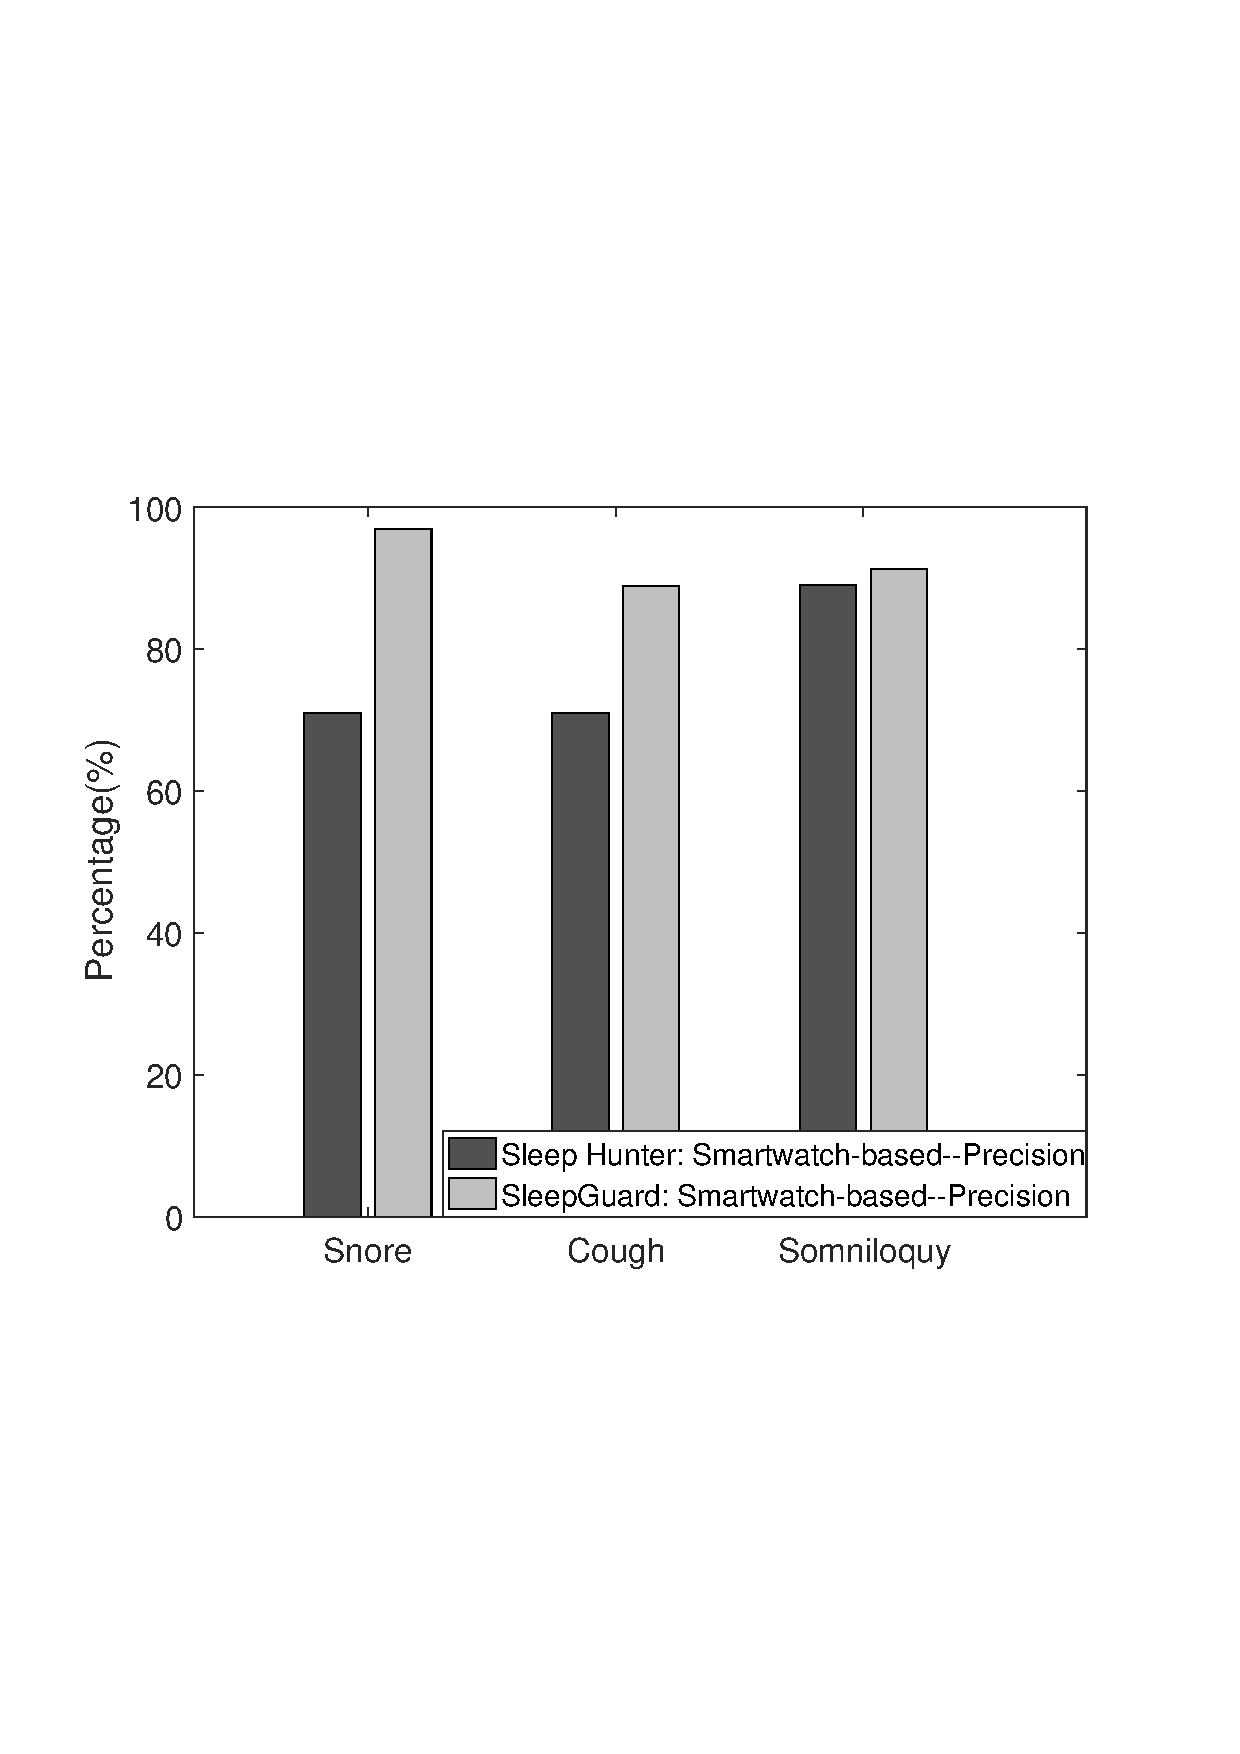
\includegraphics[width=3.6cm,height=2.7cm]{Figures/compare_sound21.pdf}}
	%\subfigure[Recall]{\label{compare_reca}
	%	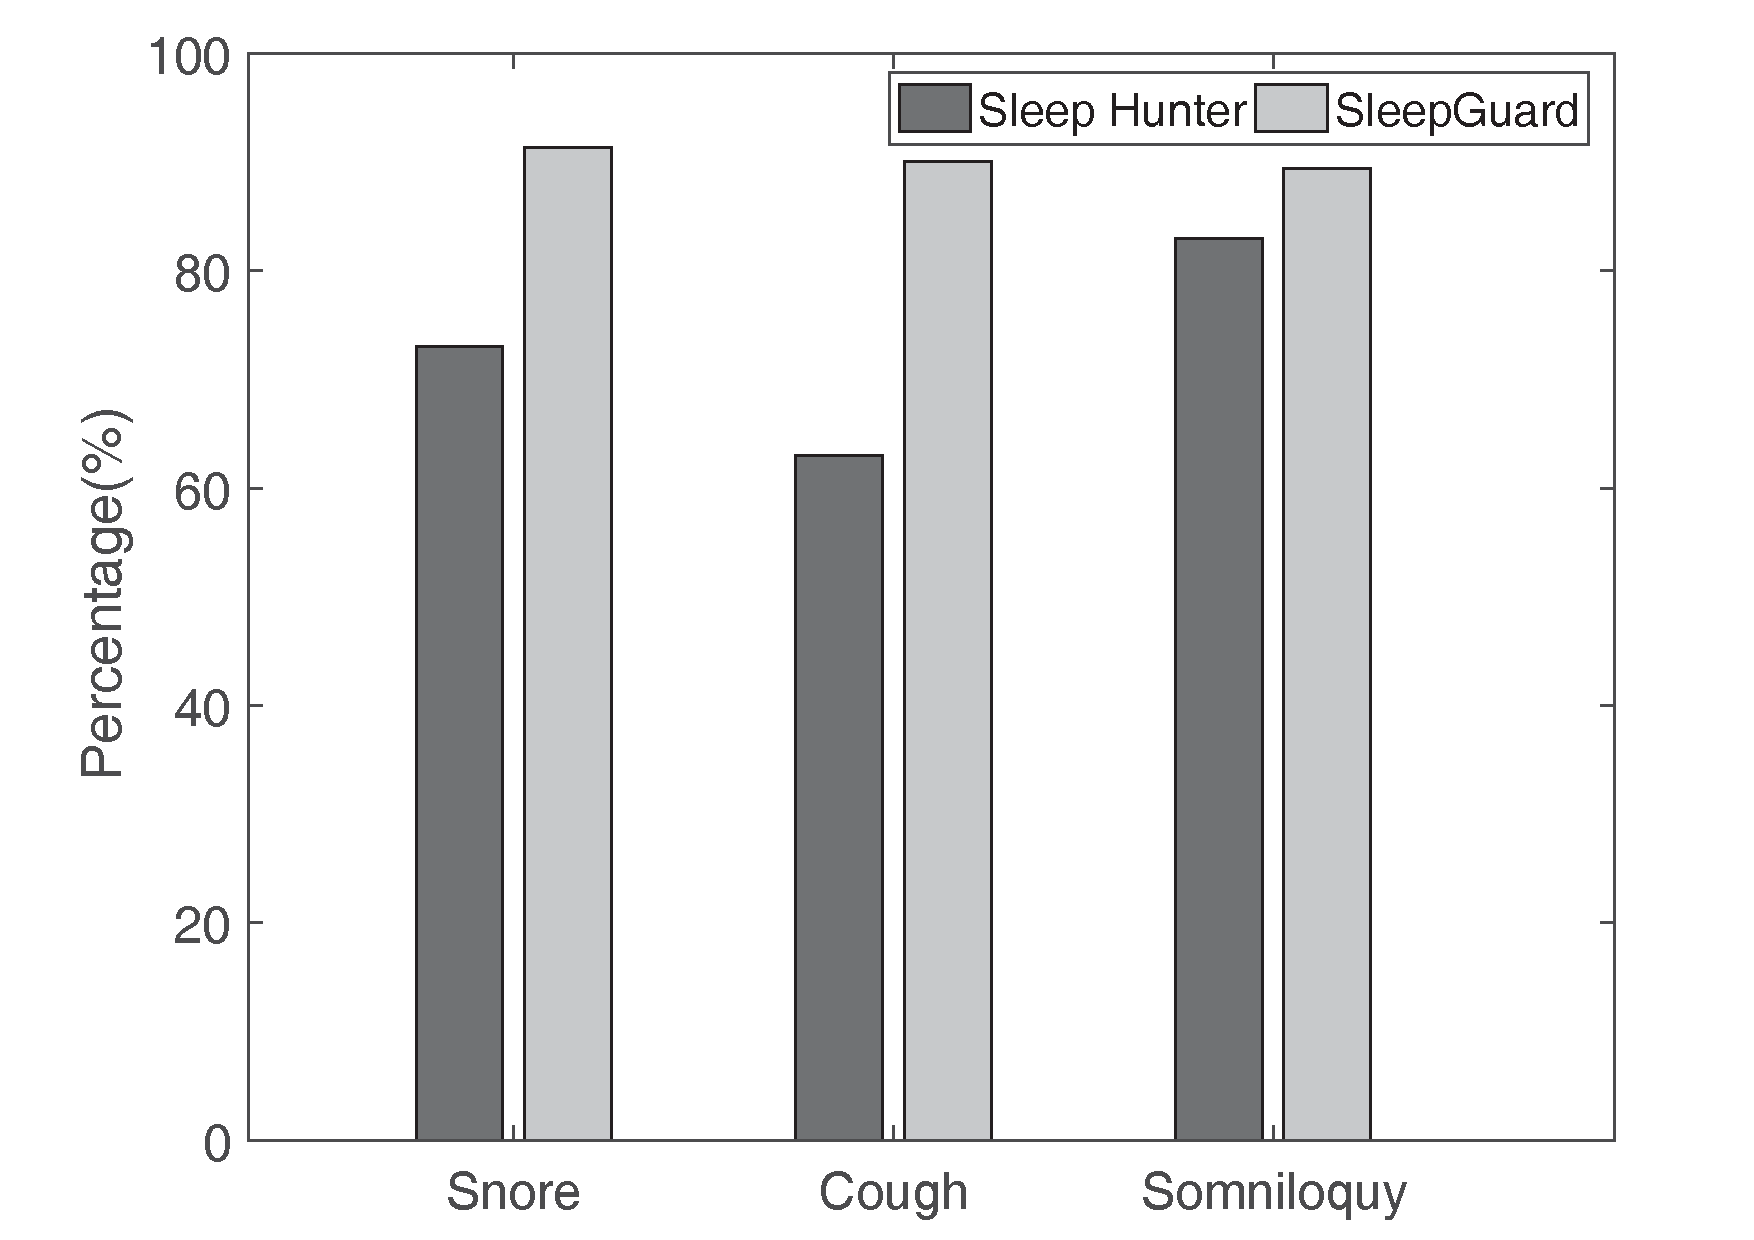
\includegraphics[width=3.6cm,height=2.7cm]{Figures/compare_sound22.pdf}}
	%\caption{Smartwatch based acoustic event detection comparison.}\label{fig:compare_sound1}
%\end{minipage}
%\begin{minipage}{.48\columnwidth}
 %   	\subfigure[Precision]{\label{compare_prec}
	%	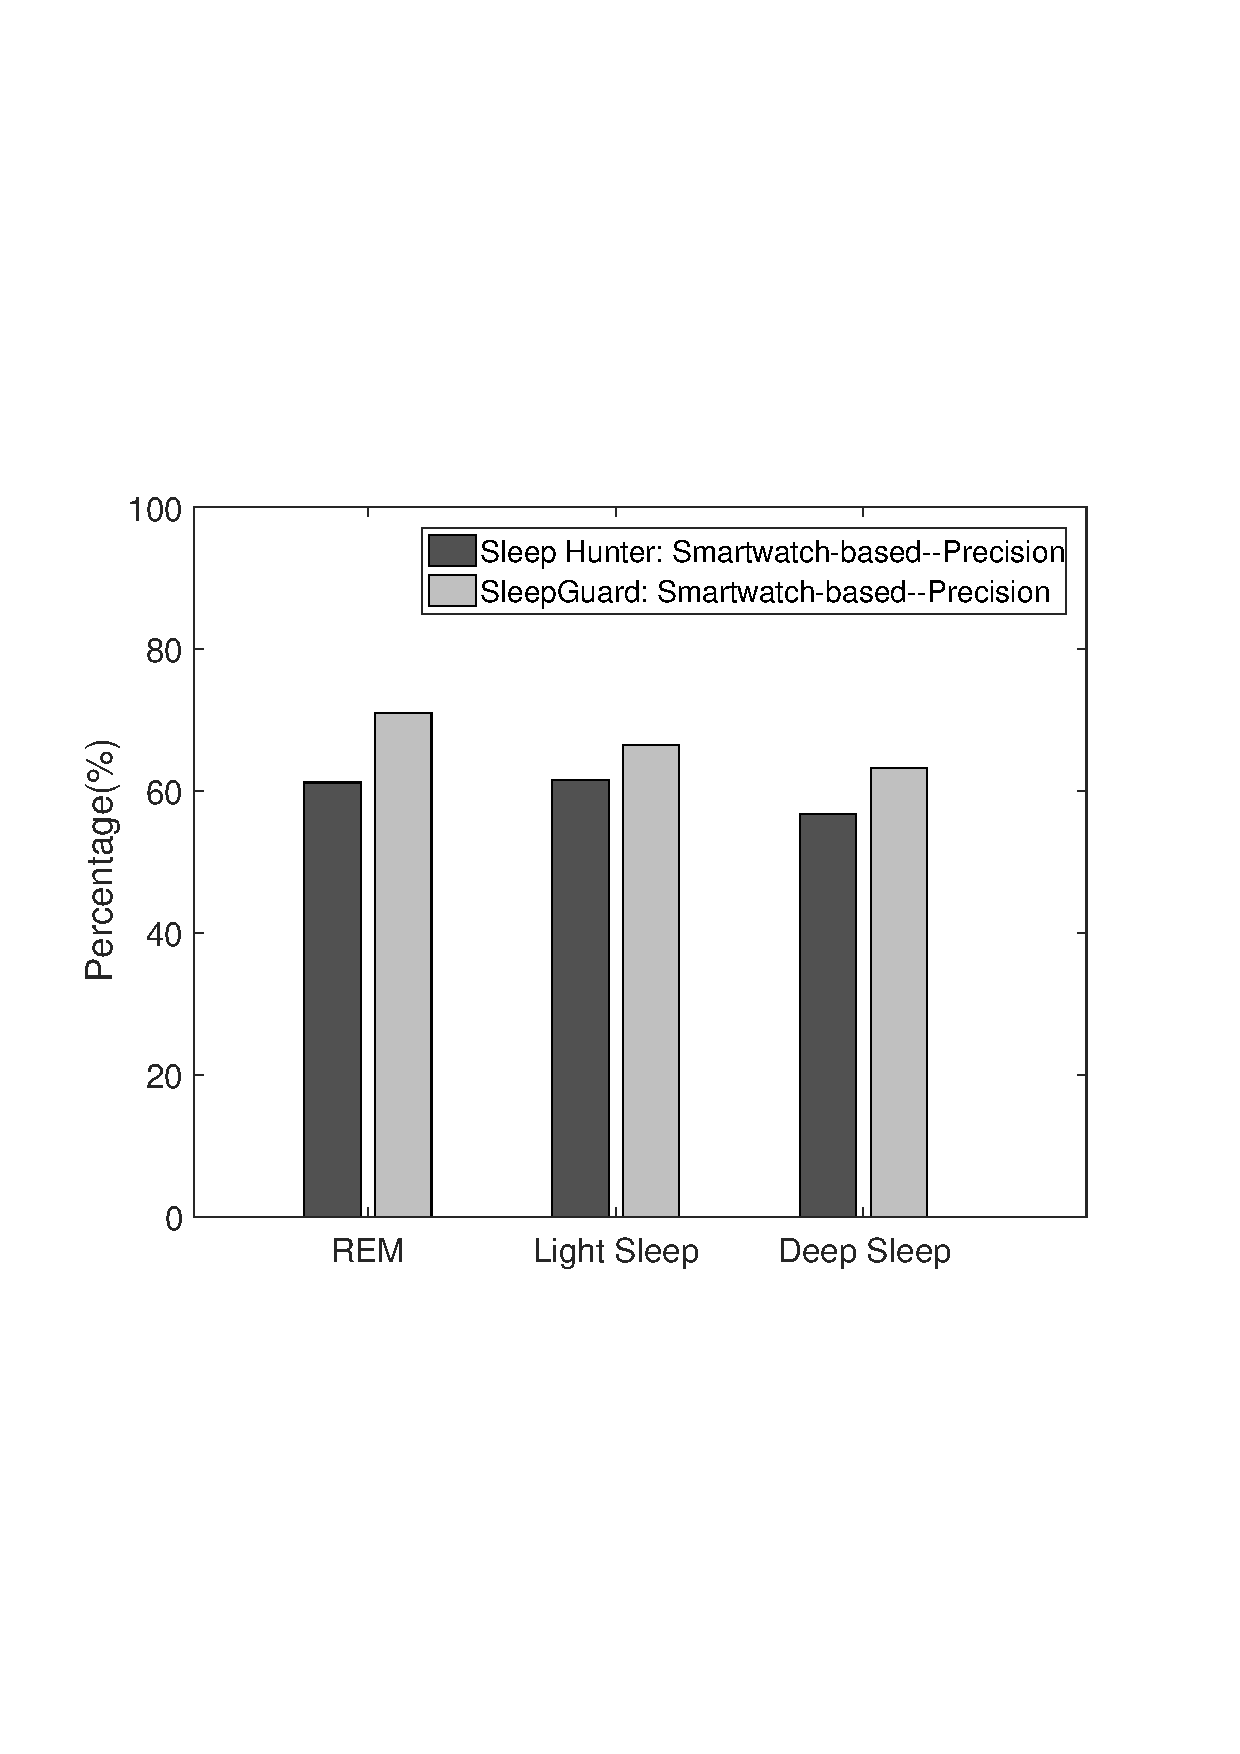
\includegraphics[width=3.6cm,height=2.7cm]{Figures/compare_stage21.pdf}}
%	\subfigure[Recall]{\label{compare_reca}
%		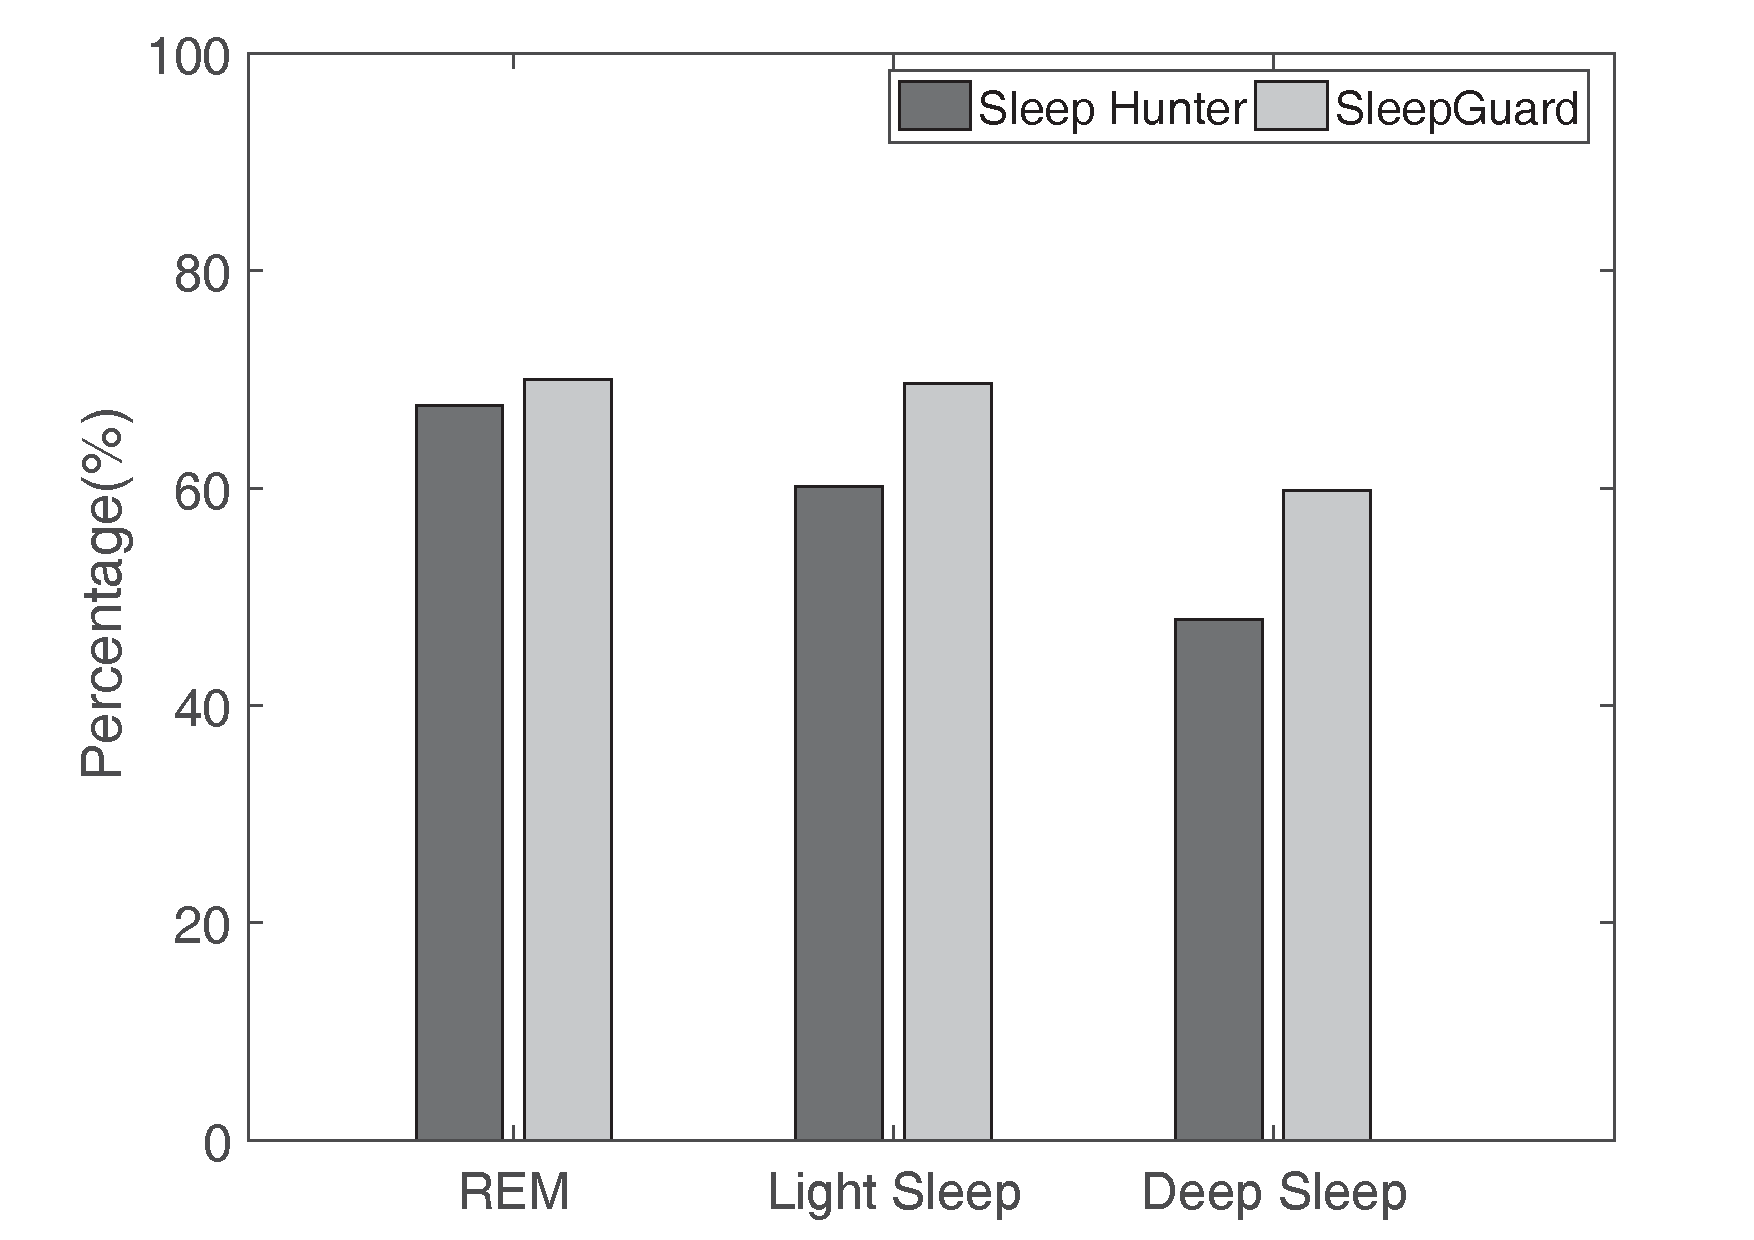
\includegraphics[width=3.6cm,height=2.7cm]{Figures/compare_stage22.pdf}}
%	\caption{Smartwatch based sleep stage detection comparison.}\label{fig:compare_stage1}
%\end{minipage}
%\end{figure*}

\begin{table}[!t]\footnotesize
 	\centering
 	\renewcommand\arraystretch{0.3}
 	\caption{Smartwatch based acoustic event detection comparison.}\label{tab:compare_sound1}
 	\begin{tabular}{c| c | c | c | c | c | c | c |}
 		\cline{2-8}
 		&\multicolumn{1}{ c|}{ }
 		&\multicolumn{2}{ c|}{ }
 		&\multicolumn{2}{ c|}{ }
         &\multicolumn{2}{ c|}{ }\\
 		&\multicolumn{1}{c|}{}
 		&\multicolumn{2}{c|}{\textbf{\footnotesize Snore}}
        &\multicolumn{2}{c|}{\textbf{\footnotesize Cough}}
 		&\multicolumn{2}{c|}{\textbf{\footnotesize Somniloquy}} \\
 		\cline{2-8}
 		\multicolumn{1}{c|}{\textbf{}}
 		&  \multicolumn{1}{c|}{\diagbox{System}{Event}}
 		&  \multicolumn{1}{c|}{\footnotesize Precision}
 		&  \multicolumn{1}{c|}{\footnotesize Recall}
        &  \multicolumn{1}{c|}{\footnotesize Precision}
 		&  \multicolumn{1}{c|}{\footnotesize Recall}
 		&  \multicolumn{1}{c|}{\footnotesize Precision}
 		&  \multicolumn{1}{c|}{\footnotesize Recall}\\
 		\cline{2-8}
 		& & & & & & &\\
 		&   \textbf{\footnotesize {\systemname}}   & $96.9\%$    &   $91.4\%$      &   $88.9\%$      &   $90.1\%$  &   $91.3\%$  &   $89.4\%$ \\
 		& & & & & & & \\
 		\cline{2-8}
 		& & & & & & &\\
 		&   \textbf{\footnotesize Sleep Hunter}   &   $71.0\%$      &   $73.0\%$     &   $71.0\%$      &   $63.0\%$   &   $89.0\%$  &   $83.5\%$\\
 		& & & & & & & \\
 		\cline{2-8}
 	\end{tabular}
 \end{table}

\begin{table}[!t]\footnotesize
 	\centering
 	\renewcommand\arraystretch{0.3}
 	\caption{Smartwatch based sleep stage detection comparison.}\label{tab:compare_stage1}
 	\begin{tabular}{c| c | c | c | c | c | c | c |}
 		\cline{2-8}
 		&\multicolumn{1}{ c|}{ }
 		&\multicolumn{2}{ c|}{ }
 		&\multicolumn{2}{ c|}{ }
        &\multicolumn{2}{ c|}{ }\\
 		&\multicolumn{1}{c|}{}
 		&\multicolumn{2}{c|}{\textbf{\footnotesize REM}}
        &\multicolumn{2}{c|}{\textbf{\footnotesize Light Sleep}}
 		&\multicolumn{2}{c|}{\textbf{\footnotesize Deep Sleep}} \\
 		\cline{2-8}
 		\multicolumn{1}{c|}{\textbf{}}
 		&  \multicolumn{1}{c|}{\diagbox{System}{Stage}}
 		&  \multicolumn{1}{c|}{\footnotesize Precision}
 		&  \multicolumn{1}{c|}{\footnotesize Recall}
        &  \multicolumn{1}{c|}{\footnotesize Precision}
 		&  \multicolumn{1}{c|}{\footnotesize Recall}
 		&  \multicolumn{1}{c|}{\footnotesize Precision}
 		&  \multicolumn{1}{c|}{\footnotesize Recall}\\
 		\cline{2-8}
 		& & & & & & &\\
 		&   \textbf{\footnotesize {\systemname}}   & $71.0\%$    &   $70.0\%$      &   $66.5\%$      &   $69.6\%$  &   $63.3\%$  &   $59.8\%$ \\
 		& & & & & & & \\
 		\cline{2-8}
 		& & & & & & &\\
 		&   \textbf{\footnotesize Sleep Hunter}   &   $61.2\%$      &   $67.6\%$     &   $61.5\%$      &   $60.2\%$   &   $56.8\%$  &   $47.9\%$\\
 		& & & & & & & \\
 		\cline{2-8}
 	\end{tabular}
 \end{table}



We also implement the algorithms employed by Sleep Hunter and apply them to the data collected using our smartwatch. This experiment allows us to check if the better performance of {\systemname} is due to the use of a smartwatch instead of a mobile phone.

For body movement detection, applying the algorithms employed by Sleep Hunter to our smartwatch data gives a comparable accuracy of around 96\% when the system only identify between drastic and small body movements. However, Sleep Hunter doesn't work when we need to detect finer-grained body movements.  {\systemname} outperforms Sleep Hunter by delivering an accuracy of drastic body movements around 90\% (see Table~\ref{tab:rollver}) and an accuracy of finer-grained body movements more than 78\% (see Fig.~\ref{fig:micro_combine}). For acoustic event detections, we apply the Sleep Hunter algorithms to detect snore, cough and somniloquy. The results in Table \ref{tab:compare_sound1} suggest that {\systemname} gives better performance over Sleep Hunter in detecting these acoustic events. Finally, we apply the sleep stage detection model used by Sleep Hunter to combine sleep-related events to identify sleep stages. The results are shown in Table \ref{tab:compare_stage1}. Again,  {\systemname} outperforms the Sleep Hunter model with a higher accuracy and recall.


This experiment confirms that the algorithms used by Sleep Hunter for sleep event and stage detection are not tuned for the smartwatch. Compared to Sleep Hunter, {\systemname} can detect sleep events and stages with a higher accuracy using a set of carefully designed methods target to target smartwatch.


\subsubsection{User survey}\label{sec:user_survey}

To understand and verify how the additional information captured by {\systemname} supports users, at the end of the experiments the participants are administrated a survey to the participants asking about their experiences with {\systemname} and their personal sleeping patterns. We combine these results with the subjective sleep quality estimates obtained through the PSQI questionnaires administered during the study. We considered two groups of users in our survey. As the main source of information, we consider the $15$ participants in our experiments who were asked about their experiences with {\systemname}, their subjective sleep quality assessment, and details of their personal sleep patterns. This set of users was augmented with external participants who were asked about their interested in the events that {\systemname} is capable of detecting. The questions in our survey include:
\begin{enumerate}
  \item Subjective sleep quality (5-levels, 1 for excellent and 5 for worst),
  \item Sleep duration,
  \item Sleep disturbances,
  \item Daytime dysfunction.
\end{enumerate}
For the above four items, each one is rated on a 1 to 5 scale. These scores are first summed to yield a total score, which ranges from 0 to 20. Then we merge every five neighboring scores into one scale and eventually divide the total scores into four levels, recorded as 0, 1, 2 and 3, representing poor, general, good and excellent, respectively. This step is necessary to compare the results of the user survey against the sleep quality estimation provided by {\systemname} and Fitbit.

\begin{table} \tiny
  \centering \caption{{Results of sleep quality assessments. The first three rows show the sleep quality scores of the different systems (mean and standard deviation) for each user across $14$ days, whereas the last two rows  compare sleep quality labels between subjective assessments and those returned by {\systemname} and FitBit. }}\label{tab:quality}
\begin{tabularx}{\textwidth}{X cccccccccccccccc }
        \toprule
         \textbf{User ID} & 1 & 2 & 3 & 4 & 5 & 6 & 7 & 8 & 9 & 10 & 11 & 12 & 13 & 14 & 15\\
         \midrule
         \rowcolor{Gray}{\systemname} & 3 (1.8) & 3 (1.5) & 0 (1.0) & 1 (1.8) &  2 (1.2) &  2 (1.7) &  3 (1.0) & 0 (1.3) &  2 (1.3) &  2 (1.0) & 2 (0) & 2 (1.5) &  1 (1.8) &  0 (1.0) &  2 (1.3)\\
         Fitbit & 3 (1.7) & 3 (2.2) & 0 (1.3) & 0 (1.8) & 1 (2.2) & 3 (1.8) & 2 (1.9) & 3 (1.8) & 2 (1.7) & 2 (1.9) & 2 (1.3) & 2 (2.0) & 2 (2.3) & 1 (1.8) & 2 (1.7) \\
         \rowcolor{Gray} User score & 3 (0.0) & 2 (1.4) & 0 (0.0) &  0 (1.7) & 2 (1.7) &  2 (1.0) & 3 (1.0) & 1 (1.7) & 1 (1.4) & 2 (1.0) &  2 (1.0) & 3 (2.0) & 0 (1.8) & 0 (1.0) & 2 (1.0) \\
         User score matching ({\systemname}) & P&O&P&O&P&P&P&O&O&P&P&O&O&P&P\\
         \rowcolor{Gray} User score matching (Fitbit) & P&O&P&P&O&O&O&\textbf{B}&O&P&P&O&\textbf{B}&O&P     \\
         \bottomrule
\end{tabularx}
\end{table}

In Table \ref{tab:quality}, we show the mean sleep quality score across 14 days given by each user together with the estimations produced by {\systemname} and Fitbit. We also give the standard deviation of the scores across the 14-day period per user. This number is given in the brackets next to the mean score. The last two rows in Table~\ref{tab:quality} compare the estimation given by {\systemname} and Fitbit against the user self-rating score. In these two specific rows, a label of `P' indicates an estimated score perfectly matches the user score, a label of `O' means the estimation error is within one scale point (for example, {\systemname} rates the user sleep to be excellent while the user's self-rating is good), and a label of `B' indicates the estimation error is greater than a scale point. As can be seen from the table, the estimation given by {\systemname} is more likely to match the user's self-rating compared to Fitbit (as indicated by having more `P' labels - 9 vs 6 ) and, unlike Fitbit, the estimation error given by {\systemname} is never greater than one scale point. To further validate this, we calculated the Spearman $\rho$-correlation~\cite{richardson2015nonparametric} between the user scores and each of the two systems, {\systemname} and Fitbit. {\systemname} provides higher correlation coefficient ($\rho = 0.842$) than Fitbit ($\rho = 0.500$). The difference in correlation was found statistically significant using a one-tailed test carried out through a Fisher r-z transformation ($Z = 1.66, p < 0.05$).  In summary, {\systemname} thus gives a better sleep quality assessment compared to Fitbit in our evaluation.

While the results above demonstrate that {\systemname} is capable of accurately estimating sleep quality, the main benefit from {\systemname} compared to previous works is not its sleep quality performance but its capability to analyze and capture the {\em root cause} of sleep issues. To demonstrate this, we carried out a follow-up analysis where we examined the events captured by {\systemname} for each of the six users assessing their sleep quality negatively (poor or general subjective quality, i.e., rating 0 or 1 in Table~\ref{tab:quality}). For four of the six users, we were able to find clear causes for their poor sleep. For one of the users, {\systemname} indicated difficulties in falling asleep, which was reflected in a high body rollover count. Further analysis of captured events indicated ambient noise and lighting to be most likely reasons for this participant. Another user complained of feeling of numbness in the arm after sleep. Events captured by {\systemname} showed that this was likely due to bad hand posture as the person tended to put the hand on top of the head before sleeping. The third user complained of frequent nightmares. Analysis of {\systemname} events showed that the person habitually slept on the left side, which has been shown to have the higher risk on nightmares~\cite{nightmare}, and often placed a hand on top of the chest, which creates additional pressure and can lead to nightmares. Finally, one of the users mentioned suffering from long-term snoring problems, which we also were able to detect from the events captured by {\systemname}. The events also highlighted that the person was often sleeping in the supine position, which further increases susceptibility to snoring-related problems. Existing systems are only capable of capturing some of these factors influencing sleep quality and thus they are not capable of providing a holistic view of the participant's sleep quality, whereas {\systemname} is capable of providing very detailed information about sleep events. To further demonstrate the benefits of {\systemname} compared to previous works, we asked the 15 participants to make appropriate adjustments according to our recommendations and to conduct a return visit survey three weeks later. It was found that some of the users were able to reduce symptoms and to improve their average quality of sleep based on the suggestions.
	
As for the user experience, results from the survey highlighted a strong interest in the information captured by {\systemname}. In particular, 80\% of participants believe that the detection of sleep posture is very necessary, showing their sleep posture can not only help people to avoid health problems caused by long-term improper sleeping posture, but also help us find out the reasons for the next day's physical discomfort, such as dizziness, muscle soreness may be due to improper sleeping posture. And there are some users are troubled by snoring. This may be due to improper sleeping posture. We map the detected snoring event and sleeping posture to suggest the user to modify his posture to a suitable posture to reduce the harm caused by long-term snoring. 60\% of the participants thought it useful to detect the hand position in supine posture, even one user mentioned that he did often have nightmares and our system found his hand was often placed on his chest, and then {\systemname} could remind him that he should take some measures to avoid such a position and thus reduce the poor sleep quality that nightmare brings. Only 20\% of participants found it useful to calculate the number of body rollover. However, detection of rollovers is useful in segmenting sleep stages. Furthermore, body rollover counts could be used to derive additional information to the user, such as how restless or peaceful the sleep has been overall.




\section{DISCUSSION}\label{sec:discussion}

In this paper, we have shown that sensors available on off-the-shelf smartwatches can be used to capture rich information about sleep
quality and factors affecting it. The main focus of our work has been to develop the required algorithms for capturing rich sleep related
information as accurately as possible. While the recognition performance of our system is very encouraging, there are some issues that
would need to be addressed in our system before larger-scale deployment would be feasible. Below we highlight the main issues and briefly
discuss possible ways to overcome them.


\cparagraph {The accuracy of sleep stage detection} \rt{In our experiment, we were unable to directly compare \systemname against medical-grade
      solutions for sleep stage detection due to lack of suitable clinical environments and expertise.} However, we would expect polysomnography to provide better sleep stage detection performance. This is because polysomnography monitors and analyzes sleep
      based on information that directly correlates with sleep such as EEG, EMG, EOG, and oxygen saturation, whereas {\systemname}
      estimates sleep quality from cues that have an indirect effect on sleep quality. In particular, \systemname only combines the body
      movement, acoustic events, sleep environment and other events during sleep to predict the sleep stage. Therefore, {\systemname} is
      not a replacement for professional medical equipment for high-precision sleep detection, but serves as a personal technology that
      provides easy-to-use and non-intrusive way to monitor personal sleep patterns and to obtain feedback about the sleep quality.
      Moreover, it can trace back to the real causes affecting sleep quality, and guide users to have the direction to improve sleep
      quality. \rt{Nonetheless, in future work, we strive to perform further studies and compare \systemname against a polysomnography-based solution.}

\cparagraph{Battery life} A critical design requirement for sleep detection is that the monitoring can operate sufficiently long to
      cover the entire duration of the user's sleep. Battery capacity on smartwatches is rather limited, resource consumption needs to be
      optimized by considering both the data collection and analysis phases. In our experiments we demonstrated that additional devices
      in the vicinity of the smartwatch can be taken advantage of, for example, some of the sensing and processing tasks can be offloaded
      to smartphones or other smart devices located within sufficient proximity. Particularly the acoustic event detection could be
      offloaded to smartphones that are located on the bedside table or elsewhere in the user's vicinity as smartphones increasingly
      integrate co-processors for audio processing that allow performing the audio event detection with a small energy footprint. We have
      also designed our analysis techniques to be as lightweight as possible to minimize energy consumption. Further improvements can be
      achieved by designing dynamic duty cycling strategies that reduce sampling during periods of regularity, and by using simple
      triggering mechanisms, such as a motion intensity detector to reduce processing overhead. Exploring these techniques is part of our
      future work.


\cparagraph{Sensor data} One limitation of {\systemname} is that we have not taken advantage of heart rate when determining the
      current sleep stage of the user. The main reason for this is programming limitations of the Huawai Smartwatch 2 device used in the
      experiments. Specifically, the device does not support querying heart rate information, but only provides it through a dedicated
      application. The output of this application is unfortunately not sufficiently accurate for sleep monitoring purposes, and restricts
      the rate at which information can be acquired. To compensate for the lack of heart rate data, \systemname considers the respiratory
      amplitude detected from accelerometer instead. As shown in our experiments, the respiratory amplitude detection significantly
      improves the performance of the sleep stage detection.

\cparagraph{Single wrist sensor}
 In our paper, we only use the sensor data of only one wrist, which loses efficiency for detecting specific events of the other wrist. Even
 so, it can achieve accurate sleep quality assessment result. Although movement patterns of the left and right wrist can be different
 during sleep, the technique used for detecting sleep related behaviors is the same. Some sleep related events like the sleep posture, body
 rollover, acoustic events, illumination 	conditions, are not affected by different wrists. The reason is that these events are related
 to the entire body rather than the part 	of the body. To adapt our approach to these sleep events, the only thing we need to do is
 adjusting new experimental parameters when the smartwatch is worn on a different wrist. For the hand position detection and micro-body
 movement detection (including the arm 	raising and hand movement), wearing the smartwatch on a different wrist does have an impact. This
 is because the hand movement 	probability and frequency are different on different hands. However, the degree of impact on our detection
 performance varies from 	person to person and can be largely cancelled through calibration. This is where we need to measure and
 consider in our future work. Alternatively, multi-sensor designs, such as combination of smart watch and intelligent ring, could be used
 to gather relevant sensor measurements from both wrists. Using an intelligent ring could also help in gathering heart rate information
 during the sleep. Exploring such multi-sensor designs is an interesting future research direction.

\cparagraph{Comparing to Fitbit} In addition, when we use Fitbit as groundtruth, Fitbit is worn on a different
      wrist from {\systemname}. However, from the analysis of the basic principles of sleep stage detected by {\systemname} and Fitbit,
      it can be found that this does not have much effect on our assessment of the results. Both Fitbit and {\systemname} have common
      grounds for detecting sleep stages based on acoustic events, the occurrence and frequency of physical activity, but we go further
      to conduct more fine-grained detection and classification of these events, and add more consideration about illumination conditions
      and respiratory amplitude. One thing we can know is that the measurement of events such as acoustic events, body rollover events,
      body tremble, etc., has little to do with the sensor data collected from the left or right hand. The major difference that may
      exist is these rich events added in {\systemname}, such as hand position, sleep posture, etc,  but these are not detected by
      Fitbit, so they have no effect when compared. Moreover, we also did a test experiment. The smart watches were worn on the left and
      right hands respectively and the event detection algorithm in {\systemname} was mainly used to detect those events that are of
      concern in Fitbit. We can see that the results are not much different. Therefore, in the end, in order to ensure that the user's
      sleep is as uncomfortable as possible, we choose to make Fitbit and Smartwatch are worn on different hands.

%  \item \textbf{Multiple sleepers}
%  Currently, {\systemname} considers that the user is sleeping alone, but there are still more complicated situations in reality, such as sleeping with a bed partner, baby, and/or a pet. However, because {\systemname} is based on the detection of smartwatch, Unlike smartphone placed on the bed, it can show more sensitivity to the user's own activities. Therefore, for the detection performance of sleeping posture, body rollover and hand position events has almost no effect, but it may have some influence on the body micro movements and acoustic events. When people around us have relatively large movements, such as body rollover, they may fluctuate to users, making it possible for us to mistakenly detect it as user's micro movements. For this kind of situation, we can test the change of acceleration data in multi-sleeper situations by popularizing the experiment to adjust the detection threshold of our body's micro movements and achieve better detection performance. This will also be a direction for our future work. As for acoustic events, we can further limit conditions, such as training the different magnitudes of the energy of the sound signals collected by the user's hand at different positions to identify whether it is the user's own acoustic event or the sound of the bed partner. In addition, the related acoustic events of the bed partner can also be considered as a factor affecting the user's sleep.

%  \item \textbf{Occurrence probability of unusual arm's positions.}
%  We detect sleep posture based on arm's positions and focus on three specific positions when detecting the position of the hand. In sleep position detection, we are based on the assumption that between the user's arms position and sleeping postures that the arms have common and (reasonably) stable positions in each posture and we consider as many possible arm positions as possible in four sleeping postures, which are the most common arm's positions for users during sleep. In hand position detection, we chose the three most representative locations that do have an impact on sleep and health. But we know that not all users or a user will not have these common positions all the time. These unusual arm's positions may cause the performance of our sleep posture detection algorithm to degrade. But of the 15 participants we tested, we can see from the video that the unusual arm's positions are present, but these are basically a slight evolution of the common positions, which have little effect on the detection of the sleeping posture. Only a small part of the unusual position will cause us to produce false positives. For this issue, we will expand the test population to further measure the impact of unusual arm's position on our system and consider more hand positions in future work.

\cparagraph{Multiple-sleeper scenario} Currently, {\systemname} considers that the user is sleeping alone, but
  there are still more complicated situations in reality, such as sleeping with a bed partner, baby, and/or a pet. However, because
  {\systemname} is based on the detection of smartwatch, Unlike smartphone placed on the bed, it can show more sensitivity to the user's
  own activities. Therefore, for the detection performance of sleeping posture, body rollover and hand position events has almost no
  effect, but it may have some influence on the body micro movements and acoustic events. When people around us have relatively large
  movements, such as body rollover, they may fluctuate to users, making it possible for us to mistakenly detect it as user's micro
  movements. For this kind of situation, we can test the change of acceleration data in multi-sleeper situations by popularizing the
  experiment to adjust the detection threshold of our body's micro movements and achieve better detection performance. This will also be
  a direction for our future work. As for acoustic events, we can further limit conditions, such as training the different magnitudes of
  the energy of the sound signals collected by the user's hand at different positions to identify whether it is the user's own acoustic
  event or the sound of the bed partner. In addition, the related acoustic events of the bed partner can also be considered as a factor
  affecting the user's sleep.

\cparagraph{Occurrence of unusual arm's positions} We detect sleep posture based on arm's positions
  and focus on three specific positions when detecting the position of the hand. In sleep position detection, we are based on the
  assumption that between the user's arms position and sleeping postures that the arms have common and (reasonably) stable positions in
  each posture and we consider as many possible arm positions as possible in four sleeping postures, which are the most common arm's
  positions for users during sleep. In hand position detection, we chose the three most representative locations that do have an impact
  on sleep and health. But we know that not all users or a user will not have these common positions all the time. These unusual arm's
  positions may cause the performance of our sleep posture detection algorithm to degrade. But of the 15 participants we tested, we can
  see from the video that the unusual arm's positions are present, but these are basically a slight evolution of the common positions,
  which have little effect on the detection of the sleeping posture. Only a small part of the unusual position will cause us to produce
  false positives. For this issue, we will expand the test population to further measure the impact of unusual arm's position on our
  system and consider more hand positions in future work.

\cparagraph{Actionable feedback} The current version of {\systemname} has been designed to provide simple recommendations on how users
should improve their sleeping environment and habits. These can be linked with additional suggestions that may alleviate the causes. For
example, problems in falling asleep can be mitigated by doing some exercise before going to bed or by going to sleep with soft music that
can be automatically turned off. Similarly, we can identify poor postures and hand positions and give feedback on what the users should aim
to improve to reduce sleep problems. For example, \cite{posture} present an anti-supine device mimicking the so-called "tennis ball
technique" to control sleep posture, in order to improve OSA hypopnoea syndrome.  For some problems, such as persistent snoring or
coughing, our system can provide suggestions such as how to improve posture to mitigate these problems, or potentially detect severe cases
where medical intervention would be appropriate. Indeed, for long term snoring the medical guidelines suggest undergoing a physical
examination so that they can timely discover possible physical diseases that may cause snoring, such as high blood pressure, cardiovascular
and cerebrovascular diseases.

\section{RELATED WORK}\label{sec:5related}

Sleep quality is a crucial issue for each individual, and the poor sleep would lead to numerous diseases, such as  endocrine dyscrasia, depression, immunity decline \cite{vgontzas2009insomnia,gottlieb2005association}. Thus, a lot of research works have been proposed to monitor the sleep \cite{langkvist2012sleep,hao2013isleep,bai2012will,kay2012lullaby,bain2003evaluation,pombo2016ubisleep}. Below, we summarize the related state-of-the-art research works as the following three categories.

\textbf{Medical technology based work}. Traditionally, the dedicated medical technologies, like EEG, ECG and EMG \cite{saper2005hypothalamic}, have been applied for sleep monitoring. Those technologies rely on the certain biomedical signals, such as brain wave, muscle tone and eye movement, to assess the sleep quality. For example, the EEG technology in \cite{langkvist2012sleep,oropesa1999sleep,ebrahimi2008automatic} monitors the brain waves, and then recognizes the sleep stages by leveraging unsupervised learning approaches.

Although a high accuracy achieved by those  technologies, they have two drawbacks. First, those  technologies require the dedicated medical devices, which are very expensive compared the widely available  smart watch/phone. Second, they require the users to be attached lots of sensors on the human body, which may cause a healthy person had to sleep and result in large errors.

Compared with those medical technologies, our system has two advantages. First, we only need a smartwatch, which is cost effective. Second, the smartwatch does not disturb a user's normal sleep, thus we can monitor the user's sleep quality more accurately.

\textbf{Smartphone based work}. Recently, some researchers use the smartphones for sleep monitoring \cite{hao2013isleep,bai2012will,kay2012lullaby,choe2011opportunities} . iSleep \cite{hao2013isleep} measures the sleep quality by recording the sleep-related acoustic events and evaluates the sleep quality using the Pittsburgh Sleep Quality Index (PSQI) \cite{carpenter1998psychometric}. Bai et al. \cite{bai2012will} predicts a user's sleep quality by observing the user's daily activities with the smartphone's sensor data, like the accelerometer, gyroscope, microphone, etc. Work in \cite{kay2012lullaby} leverages the smartphone sensors to record the sleep disruptors for a user. The authors in \cite{choe2011opportunities}  explore a series of opportunities to support healthy sleep behaviors based on the smartphone sensors. Several research works predict the sleep quality by using the smartphone to monitor the external  influence  factors, such as the daily activity, sleeping environment, location and family settings \cite{chen2013unobtrusive,zhang2013real}. Besides those research works, many Smartphone Apps, such as Sleep As Android \cite{SleepAndroid}, Sleep Journal \cite{SleepJournal}, YawnLog \cite{YawnLog} also have been developed to monitor a uer's sleep quality.

Those smartphone based systems, however, require placing the smartphone at a specifically location near to the user, which usually cannot be satisfied in reality. For example, Gu et al. \cite{gu2016sleep} needs the smartphone to be placed next to the user's head, and requires the smartphone keeping stationary throughout the sleeping process. But, many users do not want to place the mobile phone too close to the body due to health risk concerns  \cite{StepHealth,Quorasleep}.

Compared with the existing smartphone based systems, our system uses the commodity smartwatch for sleep monitoring. Since many users are willing to wear the smartwatch throughout the night, thus the smartwatch can remain relatively close to the user over the duration of sleep so that more user-related data can be collected. The performance of {\systemname} is better for most sleep events, and comparable to current state-of-the-art solutions for sleep stage estimation. However, the main advantage of \systemname results from its capability to capture a wider range of sleep-related events and to use this information to assess sleep quality and potential factors affecting it.  %The smartwatch also allows us to collect a richer set of information, which enables a wider range of sleep-related events and more accurate to achieve sleep detection and sleep quality assessment.

\textcolor{blue}{\textbf{Wearable device based work}. With the widely use of wearable devices, more and more researchers and industries try to  use the smartwatch or wearable-wrist for sleep monitoring \cite{bain2003evaluation,bonnet2003insomnia,pombo2016ubisleep,caviness1996myoclonus}.  The Sleeptracker
\cite{sleeptracker} is a wristwatch-shaped unit that apart from telling the time, also infers whether the user is in deep sleep, light sleep, or awake, using an accelerometer. The ubiSleep \cite{pombo2016ubisleep} joints heart rate, accelerometer, and sound signals collected into the smartwatch for noninvasive sleep monitoring. The aXbo alarm clock [9] is packaged as a stand-alone application in the form of an alarm clock that wirelessly communicates with a wrist-band unit. The Zeo \cite{caviness1996myoclonus} is similarly using an alarm clock base unit with a worn sensing device, but the latter is a headband rather than a wrist-band that based on electroencephalograph (EEG) to monitor sleep. We know Zeo has good performance in sleep stage detection compared to some wristband sleep monitoring products because products based on some biological signals like EEG are able to get more accurate and more representative sleep data than actigraphy-based \cite{Actigraphy} sleep monitoring products. However, the vast majority of biosignal-based sleep detection approaches require specialized equipment, which is high cost and complex to operate, while the approaches based on actigraphy are well adapted and user-friendly to accept and understand.}

\textcolor{blue}{Moreover, these actigraphy-based wristband devices or smartwatch Apps only can gather coarse-grained information and  do not design a model for deep understanding the relationship between a user's sleep pattern and the sensor data. For example, many smartwatch Apps, like Jawbone Up \cite{Jawbone}, FitBit \cite{fitbit}, YawnLog \cite{YawnLog} and WakeMate \cite{WakeMate}, do not show how they assess a user's sleep quality based on what kind of sensor data.} %\textcolor{blue}{In addition,  there is some work that uses wearable devices to detect certain detailed events of sleep. \cite{wear_related1}  design a cheap lowpower wrist-worn Sensors to monitor the user's sleep posture. \cite{wear_related2} detect roll-over and measure sleep quality using a wearable sensor. \cite{wear_related3} use a single chest-worn sensor to extract body acceleration and sleep position changes.}

%\textcolor{blue}{
	\textcolor{blue}{Compared with the existing smartwatch or wearable-wrist based systems, our system is a more complete sleep monitoring system, and is based only on sensors in commercial smart watches without additional hardware. It collect an extensive set of sleep-related events, many of which are not supported in prior work. And for sleep monitoring in daily life, it is more practical and will not invasion users�� normal sleep , and more and more people are willing to accept to wear watches to fall asleep, unlike other wearable devices such as chest-worn sensors, most people are still unwilling to accept to wear her to sleep. Moreover, our original intention and focus are more inclined to enable users to have a deeper and more comprehensive understanding of their sleep, explore the causes of sleep quality, and provide users with more practical advice to point them in a clear direction for improving sleep quality and being healthy.}%}
%Compared with the existing smartwatch or wearable-wrist based systems, our system can collect an extensive set of sleep-related events, many of which are not supported in prior work. Our system enables users to gain a deeper understanding of their sleep patterns and the causes of poor sleep.

%\textcolor{blue}{
	\textcolor{blue}{To summarize, as we can see from Table \ref{tab:related_work}, the advantage of {\systemname} is that it can detect more fine-grained sleep-related events to obtain more abundant sleep information, which is currently on the market for commercial or scientific research sleep monitoring system can not be achieved. And the performance of {\systemname} has been improved to some extent. Our original intention and focus are more inclined to enable users to have a deeper and more comprehensive understanding of their sleep, explore the cause s of sleep quality, and provide users with more practical advice to point them in a clear direction for improving sleep quality and being healthy. And compared with some medical technology like PSG, our advantages are inexpensive and easy to deploy at home, so it is suitable for most general public. And it does not need a large number of instruments attached to the user's body, thus it has less intrusiveness for sleep and does not require professional personnel to operate. Although the accuracy of {\systemname}'s ability to detect sleep cannot be compared to medical technology, it is enough for the average family's daily sleep monitoring needs. The most important is that we concentrates on physical activities rather than biomedical signals, so these rich physical activities detected are easily understood by users, and they can be adjusted with improved and improved sleep based on the results of monitoring.}%}


\begin{table*}[!t]
  \centering
  \small
  \caption{Summary of existing solutions.}\label{tab:related_work}
        \begin{tabular}{lcccccc}
        \toprule
        \textbf{System} & \textbf{High accuracy} & \textbf{Practicality} & \textbf{Low disruptive} & \textbf{Low cost} & \textbf{Informativeness} & \textbf{Interpretability}  \\
        \midrule
        \rowcolor{Gray} PSG     &  $\checkmark$ & &  &   & $\checkmark$ &  \\

        Smartphone solutions& &$\checkmark$ &$\checkmark$  &$\checkmark$   & & $\checkmark$ \\

        \rowcolor{Gray} Wearable solutions& &$\checkmark$ & $\checkmark$ & $\checkmark$  & & $\checkmark$ \\
        \textbf{\systemname} & &$\checkmark$ &$\checkmark$  & $\checkmark$  & $\checkmark$&$\checkmark$  \\

        \bottomrule
  \end{tabular}
\end{table*}

\section{CONCLUSIONS}
In this paper, we have presented {\systemname}, the first holistic smartwatch-based sleep monitoring solution that can simultaneously estimate sleep quality and provide rich information about sleep events, including body motions, acoustic events related to sleep disorders, and ambient illumination. To capture this information accurately, we have proposed new algorithms for extracting the relevant events from sensor information. We demonstrated the benefits of {\systemname} through rigorous benchmark experiments carried out using measurements collected from a two week trial with $15$ participants. The results of our experiments demonstrate that {\systemname} provides comparable sleep quality estimation accuracy than state-of-the-art consumer grade sleep monitors, while at the same time being able to accurately capture a rich set of information about factors influencing sleep quality. This information is particularly important for identifying possible causes of poor quality sleep and can be used to provide the user with suggestions on how to improve their sleep quality, e.g., by improving their sleep environment or behaviors surrounding sleep. We also compared the sleep quality estimates of {\systemname} against subjective self-assessments, demonstrating a high degree of correspondence.


\bibliographystyle{ACM-Reference-Format}
\bibliography{sleep_ref}

\end{document}
